%---------------------------------------------------------------------------%
%- Chapter 3: 三轴及耦合激发
%---------------------------------------------------------------------------%
\chapter{三轴及耦合激发}\label{chap:3}

%-- Section 3.1: 转动、振动和量子涨落
\setcounter{section}{0}%
\IfFileExists{Tex/Sections/sec-3-1.tex}{%
    \section{转动、振动和量子涨落}\label{sec:3-1}

在第2.4节与第2.6节中，我们建立了非轴对称原子核的玻尔四极形状坐标、主轴参考系与积分测度，剖析了势能曲面刚度、转动惯量与微观配对响应的解耦机制；而在后续第3.2节中，将进一步考察固定惯量下三轴转子绕主惯量轴的小振幅局域微扰展开。然而，面对真实实验所观测到的复杂在束能谱与电磁跃迁网络，初学者极易产生两类认识误区：一是将能谱上的自旋宇称标签误同化为经典刚体粒子在实空间中的确定几何轨道；二是把势能曲面上的静态极小点误当成原子核的实际物理构型，忽略了有限介观量子波包具有不可忽视的零点运动涨落。

作为第3章探讨三轴与多极激发动力学的总览入口，本节旨在系统厘清三个不同维度的物理概念：大范围空间取向转动、局部内禀形状振动与有限波包的量子零点涨落。我们从一维教学振子模型出发，明确恢复力常数与质量参数的物理量纲，解析零点涨落宽度的本质；继而探讨三维空间转动量子化、Casimir 能标与基态电四极矩的谱学不变量；进而阐明内禀形状坐标与欧拉取向角的分离条件及声子数标签的近似边界；深入剖析浅软势能面、多阱共存与量子隧穿在有限体系中的表象；最后平滑引出后续章节的动力学演化脉络。

\subsection{一维教学振子：恢复力、质量参数与零点涨落}\label{sec:3-1-1}

为了给多体坐标下的复杂量子涨落建立坚实的物理参照，首先考察一个沿广义标量坐标 $q$ 运动的一维教学简谐振子。设体系动能为 $T = p^2 / (2B)$，势能在局部极小点 $q = 0$ 附近作二次泰勒微扰展开：
\begin{equation}\label{eq:3-1-1d-potential}
V(q) = V_0 + \frac{1}{2} C q^2 \quad (C > 0),
\end{equation}
其中势能极小处于稳定平衡点，要求刚度系数满足 $C > 0$。

在物理量纲上，需要严格规范广义坐标与动力学参数的单位对应关系：
\begin{enumerate}
\item 广义坐标 $q$ 可以取不同的物理对象：若 $q$ 代表内禀四极形变度 $\alpha$ 或 $\beta$，则 $q$ 为无量纲量；若 $q$ 代表核表面的径向伸缩位移，则其量纲为长度（$[q] = \mathrm{fm}$）；若 $q$ 代表多极跃迁矩，则其量纲为电荷乘面积（$[q] = e\cdot\mathrm{fm}^2$）；
\item 质量参数 $B$ 决定了广义动量 $p = B \dot{q}$ 与动能 $T = p^2 / (2B)$ 的对应关系。为了使动能具备能量量纲 $\mathrm{MeV}$，质量参数 $B$ 的单位严格为 $\hbar^2 / (\mathrm{MeV} \cdot [q]^2)$（若 $q$ 无量纲，则 $B$ 的单位为 $\hbar^2 / \mathrm{MeV}$）；
\item 刚度系数（恢复力常数）$C \equiv \left( \frac{\partial^2 V}{\partial q^2} \right)_{q=0}$ 决定了势阱曲率，其物理单位严格为 $\mathrm{MeV} / [q]^2$。
\end{enumerate}

对该单自由度哈密顿量进行标准正则量子化，基本对易关系为 $[\hat{q}, \hat{p}] = i\hbar$。体系特征谐振角频率（能量标度）由质量与刚度的比值严格给出：
\begin{equation}\label{eq:3-1-oscillator-freq}
\hbar \omega = \hbar \sqrt{\frac{C}{B}} \quad (\mathrm{MeV}).
\end{equation}
基态量子波函数是定域于势阱底部的实高斯波包：
\begin{equation}\label{eq:3-1-ground-state-wf}
\psi_0(q) = \left( \frac{B \omega}{\pi \hbar} \right)^{1/4} \exp\left( -\frac{B \omega}{2\hbar} q^2 \right).
\end{equation}
基态量子期望值直接给出广义坐标的零点涨落均方根宽度：
\begin{equation}\label{eq:3-1-zero-point-fluc}
\langle q^2 \rangle_0 = \int_{-\infty}^{+\infty} |\psi_0(q)|^2 q^2 \, dq = \frac{\hbar}{2 B \omega} = \frac{\hbar}{2 \sqrt{B C}}.
\end{equation}

式~\eqref{eq:3-1-zero-point-fluc} 给出基态波包的坐标方差；其平方根就是均方根零点涨落宽度。它由所选势阱的质量与恢复力决定，是量子态自身的统计矩。不确定性原理在此仅给出乘积下界：
\begin{equation*}
\Delta q \Delta p \ge \frac{\hbar}{2} .
\end{equation*}
在物理理解与实验测量之间，需要系统澄清波包统计矩、跃迁矩阵元与测量误差的辩证关系：
\begin{itemize}
\item \textbf{波包统计矩与非对角跃迁矩阵元的完备性联系}：对于线性坐标算符 $\hat{q}$，当体系具有良好基底完备性且基态平均值 $\langle 0 | \hat{q} | 0 \rangle = 0$ 时，利用完备性求和（closure 关系）可得：
\begin{equation}\label{eq:3-1-closure-q2}
\langle 0 | \hat{q}^2 | 0 \rangle = \sum_n |\langle n | \hat{q} | 0 \rangle|^2.
\end{equation}
这表明基态波包涨落平方并非与可观测量完全割裂，它严格对应于从基态出发的跃迁响应网络强度总和。但这并不意味着可将单个非对角跃迁矩阵元 $\langle f | \hat{\mathcal{M}} | i \rangle$（如低激发态间的 $B(E2)$ 跃迁）直接等同于基态涨落宽度本身；
\item \textbf{量子波包宽度与经典静态极小点的本质区别}：经典力学中体系可静态定域于势能谷底 $q_0 = 0$ 且无动能涨落；在量子力学中，即使势能在原点具有极深势阱，零点振动能与基态波包弥散度 $\sqrt{\langle q^2 \rangle_0} > 0$ 始终存在。波包的统计涨落宽度与实验仪器的多普勒测量误差或谱线展宽亦分属不同范畴。
\end{itemize}

\subsection{转动量子化、Casimir 标度与谱学不变量}\label{sec:3-1-2}

当我们将上述一维几何扩展到三维多体转动时，体系呈现出全新的对称性守恒律与量子化阶梯。孤立原子核在无外场空间中满足空间各向同性，其总角动量守恒且具有固定的 Casimir 模长 $\hat{\mathbf{J}}^2 = \hbar^2 I(I+1)$。

三维刚性转子的哈密顿量写作：
\begin{equation}\label{eq:3-1-rot-H}
\hat{H}_{\text{rot}} = \sum_{k=1}^3 \frac{\hat{J}_k^2}{2\mathcal{J}_k} = \sum_{k=1}^3 A_k \mathcal{I}_k^2,
\end{equation}
其中 $\mathcal{I}_k \equiv \hat{J}_k / \hbar$ 为无量纲体轴角动量算符，$A_k \equiv \frac{\hbar^2}{2\mathcal{J}_k}$ 为能量量纲转动常数（$\mathrm{MeV}$ 或 $\mathrm{keV}$），与第3.2节中的约定严格保持一致。在具有轴对称动力学惯量 $\mathcal{J}_1 = \mathcal{J}_2 \equiv \mathcal{J}_\perp$ 且内禀投影 $K=0$ 的转动带中，转动能谱表述为：
\begin{equation}\label{eq:3-1-rot-spectrum}
E_{\text{rot}}(I) = \frac{\hbar^2}{2\mathcal{J}_\perp} I(I+1) = A_\perp I(I+1).
\end{equation}
需要明确的是，$K=0$ 条件本身仅要求角动量沿对称轴的分量为零，并不迫使自旋 $I$ 只能取偶数（正如第2.5节所严格推导的，$I$ 可取任意非负整数，每个自旋包含 $(2I+1)$ 重磁简并 $M = -I, \dots, +I$）。基带中仅出现偶数自旋序列 $I = 0, 2, 4, \dots$ 的物理前提，是内禀参考态额外具备绕垂直于对称轴的主轴旋转 $\pi$ 的离散二度轴对称性（正旋称 $R_{y, \text{intr}}(\pi) |\Phi\rangle = + |\Phi\rangle$）；若不具备该内禀离散对称性，奇数自旋同样可以存在。

在此必须厘清角动量投影量子数与模型假设的依赖关系：
\begin{enumerate}
\item \textbf{内禀投影 $K$ 的模型属性}：在理想轴对称强变形核中，自旋在内禀对称轴上的投影 $K$ 是一个优良的绝热近似量子数。然而在一般的三轴非轴对称核中（$A_1 \ne A_2 \ne A_3$），哈密顿量打破了绕单一主轴旋转的连续对称性，不同 $K$ 分量发生严重混合，$K$ 不再是守恒标签，物理态是由多个不同 $K$ 态构成的相干叠加（详见第2.5节与第3.2节）；
\item \textbf{基态静态四极矩 $Q_s(0^+) = 0$ 绝不否定核形变}：在实验谱学中，偶偶核基态的自旋宇称恒为 $I^\pi = 0^+$。根据第1.2节阐释的 Wigner-Eckart 定理，任意处于自旋为 $I$ 的态矢对二阶球张量电四极算符 $\hat{Q}_{20}$ 的对角期望值正比于 Clebsch-Gordan 系数 $(I \, 2 \, I; M \, 0 \, M)$。当自旋 $I = 0$ 时：
\begin{equation}\label{eq:3-1-WE-zero}
(0 \, 2 \, 0; 0 \, 0 \, 0) \equiv 0 \implies Q_s(0^+) = \sqrt{\frac{16\pi}{5}} \langle 0, 0 | \hat{Q}_{20} | 0, 0 \rangle = 0.
\end{equation}
式~\eqref{eq:3-1-WE-zero} 是全空间三维角动量几何耦合的必然数学结论，与原子核内禀是否发生四极形变毫无关联。即使核在内禀系具备极大的四极变形，其实验室基态各向同性取向平均后测得的静态四极矩依然严格为零。真实的内禀电四极度由实验室系转动标量不变量所确定（Kumar-Cline 形状不变量，Cline 1986，定义与第2.1节严格统一）~\cite{cline-1986-nuclear-shapes-coulomb-excitation}：
\begin{equation}\label{eq:3-1-cline-invariant}
q_2 \equiv \sqrt{5} \langle 0^+ | [\hat{Q} \times \hat{Q}]_0 | 0^+ \rangle = \sum_i |\langle i || \hat{\mathcal{M}}(E2) || 0^+ \rangle|^2 \ge 0.
\end{equation}
这一表达式使用完整中间态求和。$q_2$ 刻画所用电四极算符的均方强度；将它进一步解释为内禀振幅或形状分布，要保留第~2.1、2.4~节的条件。单个矩或少数跃迁不能代替完整分布。
\end{enumerate}

\subsection{形状振动与取向运动的坐标解耦及声子标签界限}\label{sec:3-1-3}

低能原子核结构理论在描述集体动力学时，将五维空间中的多极自由度 $\alpha_{2\mu}$（$\mu = -2, \dots, +2$）解耦为两套物理本质截然不同的运动坐标（Bohr 1952）~\cite{bohr-1952-surface-particle-coupling}：
\begin{itemize}
\item 2 个内禀几何形状变量 $(\beta, \gamma)$：刻画核椭球的径向四极拉长与三轴非轴对称横向剪切，对应核的\textbf{内禀形状振动}；
\item 3 个欧拉取向角 $\Omega = (\phi, \theta, \psi)$：确定内禀主轴坐标系相对于实验室空间的欧拉转角，对应核的\textbf{大范围整体转动}。
\end{itemize}

对于所选参考态，转动能标小于相关内禀激发能隙，是采用振转绝热近似的常用条件之一\cite{book-bohr-mottelson-nuclear-structure-vol2}：
\begin{equation}\label{eq:3-1-adiabatic-condition}
\hbar \omega_{\text{rot}} \ll \hbar \omega_{\text{vib}}.
\end{equation}
需要澄清的是，绝热分离的本质是转动时间尺度远慢于内禀响应时间尺度，由转动角速度诱导的非绝热导数耦合（如科里奥利微扰 $\langle \Phi_1 | \frac{\partial}{\partial \Omega} | \Phi_2 \rangle$）较小；这与波包几何振幅的大小（$\Delta R / R_0$）属于不同物理层次的评估。大振幅集体运动在能隙充足时依然可以保持绝热演化，而微小振幅在能级微观反交叉（pseudo-crossing）或高能级密度区域亦可诱发剧烈的非绝热混合。

在绝热近似下，转动与内禀振动波函数可表示为对称化的乘积试探形式：
\begin{equation}\label{eq:3-1-factorized-wf}
\Psi_{IM}(\beta,\gamma,\Omega)\approx\sum_K\Phi_K(\beta,\gamma)\,\varphi_{IMK}(\Omega).
\end{equation}
其中 $\varphi_{IMK}$ 是按所用Euler角、离散对称性和测度构造的转动函数；其Wigner $D$ 组合与规范化见第~2.5~节及附录B。本式只示意形状振幅与取向函数的分工，少数 $K$ 项的保留属于具体振转近似，不能视为一般三轴核的精确本征态。

基于上述分离，唯象集体模型常引入简谐声子量子数（如 $\beta$ 振动声子数 $n_\beta$、$\gamma$ 振动声子数 $n_\gamma$ 或摆动声子数 $n_w$）来标记不同能带。然而，必须清醒认识到声子数 $n$ 仅仅是局部简谐展开下的数学标签：
\begin{enumerate}
\item \textbf{势能面的强非简谐性}：真实核势能面包含高阶项（如 $\beta^4$、$\beta^3 \cos(3\gamma)$），微观质量参数与转动惯量亦强烈依赖于动态坐标 $(\beta, \gamma)$，破坏了严格简谐二次型；
\item \textbf{转动—振动耦合效应}：当转动频率增加时，离心力拉伸形变（离心拉伸效应），科里奥利力引发内部准粒子顺排，诱导转动态与振动态发生剧烈动力学杂化；
\item \textbf{整数能量比绝非模式判据}：在束谱学中，实验测得的激发能级比值（如 $E(4_1^+)/E(2_1^+) \approx 2.0$ 对应简谐振动，$E(4_1^+)/E(2_1^+) \approx 3.33$ 对应刚性转子，比值接近 $2.5$ 对应软核或 $\gamma$ 不稳定核）仅是粗糙的唯象线索，绝不能充当认定激发模式的充要判据。判定应结合具体模型框架，考察带间绝对跃迁矩阵元 $B(E2)$、跃迁选择定则以及分支比等综合指标，而不强求每一个具体核都必须测齐全部绝对跃迁强度。
\end{enumerate}

\subsection{浅软势能面、多阱隧穿与量子波包分布}\label{sec:3-1-4}

上述关于简谐振动与定常转动的图景，建立在势能曲面具有显著深势阱极小的假说之上。然而在过渡核区与软核区（如 $A \approx 130$ 核区的部分核素），这一前提往往发生动摇。

\textbf{浅软势能面与大振幅零点涨落}：在许多低能原子核中，微观约束密度泛函（CDFT）或推转微观模型计算给出的势能面沿 $\gamma$ 方向非常平缓（如 Wilets-Jean $\gamma$ 不稳定软势），或沿 $\beta$ 方向势垒极低。此时零点涨落宽度（如 $\sqrt{\langle \Delta \gamma^2 \rangle_0}$）与局部二次谐振展开的有效适用区间相当甚至超界（特别是在长轴对称平衡点 $\gamma_0 = 0^\circ$ 附近，单纯将涨落与零平衡值比较失去意义，必须与势能曲面曲率主导区开展比较）。当零点涨落横跨大范围变形区域时，势能面上的静态极小点不能代表体系的实际有效几何构型；真实物理特性完全由量子波包概率密度分布 $|\Psi(\beta, \gamma)|^2$ 在全流形上的加权分布所主导。

\textbf{多阱共存与量子隧穿}：当微观能量曲面存在多个深度相近的分立极小（例如长椭球极小与扁椭球极小共存，或球形基态与变形异能态共存）时，体系在有限势垒之间发生量子隧穿。在此情形下，体系的能量本征态不再局域于单一势阱，而是分布在两阱中的波包相干叠加形成的宏观量子干涉态（形状共存态）。

\textbf{有限体系定态与内禀对称性破缺的范畴界限}：在宏观固体或液晶中，热力学极限下无穷大自由度的集体冻结会导致实验室系出现真正的连续对称性自发破缺；然而原子核是有限介观粒子体系，连续转动对称性 $[\hat{H}, \hat{\mathbf{J}}] = 0$ 在实验室系中是不可动摇的严格守恒律。微观平均场中出现的所谓“自发对称破缺”，仅仅是变分引入的内禀单粒子波包的内部属性；通过角动量投影技术，可从微观破缺波包中提取出具有确定良好自旋量子数的试探空间态矢（good-$I$ 态）；而在该受限物理子空间中进一步通过哈密顿量 Ritz 变分（Hill-Wheeler 方程）求解，便在实验室参考系中求得满足守恒律的物理近似本征态（详见第2.5节）。

\subsection{章节脉络与后续动力学演化接口}\label{sec:3-1-5}

本节所澄清的几何取向、内禀振动与量子涨落之间的物理边界，为全书第3章展开深入的低能动力学分析提供了清晰的逻辑阶梯：
\begin{itemize}
\item \textbf{第 3.2 节（稳定转轴与摆动的局域极限）}：当四极形状势能变硬、内禀形状振动被有效冻结时，我们将坐标系完全固定于三轴椭球主轴系，深入探究经典欧拉陀螺的运动稳定性，并在局域大自旋展开下精确推导纯转子的三维摆动声子激发频率及其两种轴对称极限；
\item \textbf{第 3.3 节（准粒子顺排与横/纵向摆动分支）}：将微观壳模型费米面与未配对价核子带入集体核芯，研究高 $j$ 准粒子轨道角动量顺排如何打破主轴旋转对称性，催生出具有丰富微观指纹的横向摆动（TW）与纵向摆动（LW）分支；
\item \textbf{第 3.5 节（手征几何、隧穿与有限核态）}：当三轴非轴对称集体核芯与一个高 $j$ 价粒子和一个高 $j$ 价空穴实现非共面角动量矢量耦合时（标量三重积 $\mathbf{j}_p \cdot (\mathbf{j}_h \times \mathbf{R}) \ne 0$，并不要求三矢量严格 $90^\circ$ 正交），体系在旋转参考系诱发自发手征对称破缺，进而在有限量子隧穿作用下于实验室系形成近简并的手征双重带（Chiral doublet bands）；
\item \textbf{第 3.6 节（$\gamma$ 形状模与取向模的耦合）}：重新放宽形状冻结假设，系统探讨内禀 $\gamma$ 形状振动与欧拉三维取向运动之间的非线性动力学杂化，阐明同自旋、同宇称能带在有限能隙下如何通过非对角矩阵元诱发强烈的态混合。
\end{itemize}
%
}{%
    \section{转动、振动和量子涨落 [未完成]}\label{sec:3-1}%
    \textit{本节尚未完成。}%
}

%-- Section 3.2: 稳定转轴与摆动的局域极限
\setcounter{section}{1}%
\IfFileExists{Tex/Sections/sec-3-2.tex}{%
    \section{稳定转轴与摆动的局域极限}\label{sec:3-2}

在第2.4节与第2.6节中，我们建立了非轴对称原子核的玻尔四极形状坐标、主轴参考系定义，以及微观动能响应与转动惯量的解耦分析；在第3.1节中，阐明了非轴对称转动态由大振幅集体转动与围绕特定取向的小振幅激发复合而成的动力学架构。在处理具有稳定三轴四极形变（$0^\circ < \gamma < 60^\circ$）的原子核体系时，一个首要的物理问题是：非轴对称核在角动量守恒的约束下，究竟倾向于绕哪一个内禀主轴转动？微观流体力学结构如何决定各主轴转动惯量的相对大小？围绕稳定主轴展开的小振幅横向摇摆（wobbling motion）如何通过局域大自旋代数求解，其振动频率与两种截然不同的轴对称极限又有何深刻联系？

本节系统讨论三轴转子主轴标记体系、刚体与无旋流体转动惯量的对立机制、欧拉经典稳态与相空间拓扑分离线，并在体轴无量纲角动量反常对易代数下严格推导大自旋小振幅双横向展开与纯转子摆动频率公式。进一步辨析两种轴对称极限下的频率行为与高 $K$ 进动态界限，最后评估有限自旋非谐效应与多声子谐振假说的物理适用边界。

\subsection{三轴形变转子的主轴标记与惯量机制对立}\label{sec:3-2-1}

描述三轴形变核的几何与转动动力学，首先需要严格固定几何主轴与坐标轴的对应关系。在玻尔主轴参考系下，四极形变椭球的三个主半轴通常按几何尺度排序标记为短轴（short, $s$ 轴）、中间轴（intermediate, $m$ 轴）和长轴（long, $l$ 轴）：
\begin{equation}\label{eq:3-2-axes-order}
R_s < R_m < R_l.
\end{equation}
在标准扇区 $0^\circ < \gamma < 60^\circ$ 内，三轴形状由形变幅度 $\beta$ 与三轴不对称角 $\gamma$ 唯一确定，$\gamma = 30^\circ$ 对应最大三轴不对称度。为了开展动力学求解，通常将几何主轴映射为直角坐标轴 $(1, 2, 3)$ 或 $(x, y, z)$。定义各主轴上的转动惯量为 $\mathcal{J}_k > 0$（$k = 1, 2, 3$），相应的能量量纲转动常数定义为：
\begin{equation}\label{eq:3-2-rot-constants}
A_k \equiv \frac{\hbar^2}{2\mathcal{J}_k} \quad (k = 1, 2, 3).
\end{equation}

在低能核结构中，刚体转动与无旋流体转动代表了核质量传输的两种极端理想参考模型：
\begin{enumerate}
\item \textbf{经典刚体转动惯量模型}：若核内全部核子如同经典刚体一样随椭球形状做整体旋转，其局部速度场为 $\mathbf{v}(\mathbf{r}) = \boldsymbol{\omega} \times \mathbf{r}$。绕第 $k$ 主轴的刚体转动惯量直接由物质密度分布的二阶矩给出：
\begin{equation}\label{eq:3-2-rigid-inertia}
\mathcal{J}_k^{\text{rig}} = \int \rho(\mathbf{r}) (r^2 - x_k^2) \, d^3r \propto R_i^2 + R_j^2 \quad (i \ne j \ne k).
\end{equation}
根据几何半轴不等式~\eqref{eq:3-2-axes-order}，由两较大半轴平方和决定的转动惯量最大。因此刚体模型严格预言：绕最短几何轴 $s$ 的转动惯量最大，绕最长几何轴 $l$ 的转动惯量最小：
\begin{equation}\label{eq:3-2-rigid-order}
\mathcal{J}_s^{\text{rig}} > \mathcal{J}_m^{\text{rig}} > \mathcal{J}_l^{\text{rig}} \implies A_s^{\text{rig}} < A_m^{\text{rig}} < A_l^{\text{rig}} ,
\end{equation}
\item \textbf{流体力学无旋流转动惯量模型}：由于核子为费米子且具有强空间重叠与配对关联，原子核并非刚性刚体。在玻尔—莫特森经典集体模型中，原子核集体转动被视作不可压缩无旋理想流体的表面波运动，速度场满足无旋条件 $\nabla \times \mathbf{v} = 0$。微观动能积分直接给出无旋流体转动惯量（Bohr 1952，Bohr 与 Mottelson 1953）~\cite{bohr-1952-surface-particle-coupling,bohr-mottelson-1953-collective-individual-original}：
\begin{equation}\label{eq:3-2-irrot-inertia}
\mathcal{J}_k^{\text{irr}} = 4 B \beta^2 \sin^2\left(\gamma - \frac{2\pi}{3} k\right) \quad (k = 1, 2, 3),
\end{equation}
其中 $B$ 为四极质量参数。在标准扇区 $0^\circ < \gamma < 60^\circ$ 内，三轴惯量分布呈现强烈的 $\gamma$ 敏感性。特别地，在扇区中点 $\gamma = 30^\circ$ 附近：
\begin{equation}\label{eq:3-2-irrot-order}
\mathcal{J}_m^{\text{irr}} \propto \sin^2(90^\circ) = 1, \quad \mathcal{J}_s^{\text{irr}} \propto \sin^2(30^\circ) = \frac{1}{4}, \quad \mathcal{J}_l^{\text{irr}} \propto \sin^2(-30^\circ) = \frac{1}{4}.
\end{equation}
无旋流模型明确预言：绕几何中间轴 $m$ 的转动惯量最大，可达其余两轴惯量的 4 倍左右：
\begin{equation}
\mathcal{J}_m^{\text{irr}} > \mathcal{J}_s^{\text{irr}}, \mathcal{J}_l^{\text{irr}} \implies A_m^{\text{irr}} < A_s^{\text{irr}}, A_l^{\text{irr}}.
\end{equation}
\end{enumerate}

上述对比表明：主转动惯量排序深刻依赖于核内质量传输机制。在真实原子核中，由于残余配对关联、单粒子轨道占据与科里奥利力的复杂交织，有效转动惯量并不存在逐轴介于刚体与无旋流之间的普遍上下界包络；有效惯量的大小和方向强烈依赖于微观准粒子组态与推转频率（详见第2.6节与第3.3节）。在后续推导中，我们直接将具有最大转动惯量（最小转动常数）的主轴声明为转动主轴 1，以保持数学体系的普遍自洽。

\subsection{欧拉稳态转动与非主轴相空间分离线}\label{sec:3-2-2}

为了确定三轴核在固定总角动量下的转动稳定性，首先考察经典欧拉陀螺动力学。设转子在主轴系下的无量纲角动量分量为 $\mathcal{I}_k$（$k = 1, 2, 3$），体系哈密顿量为无外力矩转动的动能：
\begin{equation}\label{eq:3-2-classical-H}
E = \sum_{k=1}^3 A_k \mathcal{I}_k^2 = \frac{1}{2} \sum_{k=1}^3 \frac{\hbar^2 \mathcal{I}_k^2}{\mathcal{J}_k}.
\end{equation}
在孤立体系中，总角动量模长严格守恒，角动量矢量端点被严格限制在半经典角动量球面上：
\begin{equation}\label{eq:3-2-I-sphere}
\mathcal{I}_1^2 + \mathcal{I}_2^2 + \mathcal{I}_3^2 = I^2.
\end{equation}

设主轴按惯量大小降序排列为 $\mathcal{J}_1 > \mathcal{J}_2 > \mathcal{J}_3$，即转动常数满足：
\begin{equation}\label{eq:3-2-A-order}
A_1 < A_2 < A_3.
\end{equation}
在固定总角动量模长且三个惯量互异的前提下，能量曲面在三条主轴上的极值与稳定性具有完全不同的拓扑性质：
\begin{enumerate}
\item \textbf{最大惯量轴 1}（$\mathcal{I}_1 = \pm I, \mathcal{I}_2 = \mathcal{I}_3 = 0$）：能量取全域严格局域极小值 $E_{\min} = A_1 I^2$。微小横向扰动受到正曲率恢复力的约束，角动量矢量在相空间中围绕该轴形成闭合的稳定轨道，属于线性稳定。在量子体系中，该状态对应给定自旋 $I$ 下能量最低的 yrast 态分支；
\item \textbf{最小惯量轴 3}（$\mathcal{I}_3 = \pm I, \mathcal{I}_1 = \mathcal{I}_2 = 0$）：能量取全域严格局域极大值 $E_{\max} = A_3 I^2$。微小扰动同样受封闭轨道约束，线性稳定，但它对应高能分支，并非固定自旋的最低能（yrast）分支；
\item \textbf{中间惯量轴 2}（$\mathcal{I}_2 = \pm I, \mathcal{I}_1 = \mathcal{I}_3 = 0$）：能量处于双曲鞍点，是线性不稳定的。在经典相空间中，通过该鞍点的能量等值线构成分离线（separatrix），将相空间严格划分为围绕轴 1 旋进与围绕轴 3 旋进的两类拓扑互不相交的动力学轨道~\cite{book-raduta-coherent-states}。
\end{enumerate}

\subsection{小振幅双横向展开与纯转子摆动频率}\label{sec:3-2-3}

我们进而建立量子力学下围绕最大惯量轴 1 稳定转动的局域谐振微扰理论。设主转动轴为最大惯量轴 1，转动常数满足 $A_1 < A_2 \le A_3$，定义相对差：
\begin{equation}\label{eq:3-2-d-params}
d_2 \equiv A_2 - A_1 > 0, \quad d_3 \equiv A_3 - A_1 > 0.
\end{equation}
采用无量纲体轴角动量算符 $\mathcal{I}_k = \hat{J}_k / \hbar$，满足体坐标反常负对易关系（负号源于体坐标系相对于实验室系的相对逆旋转）~\cite{book-bohr-mottelson-nuclear-structure-vol2}：
\begin{equation}\label{eq:3-2-body-fixed-commutation}
[\mathcal{I}_a, \mathcal{I}_b] = -i \epsilon_{abc} \mathcal{I}_c \implies [\mathcal{I}_2, \mathcal{I}_3] = -i \mathcal{I}_1 \approx -i I.
\end{equation}

为了与体轴系的负对易号匹配，定义产生与湮灭算符为（Bohr 与 Mottelson 1975 专著第二卷第 190 页 Eq.(4-297)）~\cite{book-bohr-mottelson-nuclear-structure-vol2}：
\begin{equation}\label{eq:3-2-boson-mapping}
a \equiv \frac{\mathcal{I}_2 - i \mathcal{I}_3}{\sqrt{2I}}, \quad a^\dagger \equiv \frac{\mathcal{I}_2 + i \mathcal{I}_3}{\sqrt{2I}}.
\end{equation}
直接验算其玻色对易子：
\begin{equation}\label{eq:3-2-boson-commutator}
[a, a^\dagger] = \frac{1}{2I} [\mathcal{I}_2 - i \mathcal{I}_3, \mathcal{I}_2 + i \mathcal{I}_3] = \frac{i}{I} [\mathcal{I}_2, \mathcal{I}_3] \approx \frac{i}{I} (-i I) = 1.
\end{equation}
反演得到横向分量的算符表达：
\begin{equation}\label{eq:3-2-transverse-coords}
\mathcal{I}_2 = \sqrt{\frac{I}{2}} (a^\dagger + a), \quad \mathcal{I}_3 = i \sqrt{\frac{I}{2}} (a - a^\dagger).
\end{equation}

在大自旋极限下，将量子哈密顿量以固定自旋 Casimir 项 $A_1 I(I+1)$ 为基线展开：
\begin{align}
\hat{H} &\approx A_1 I(I+1) + d_2 \mathcal{I}_2^2 + d_3 \mathcal{I}_3^2 \nonumber \\
&= A_1 I(I+1) + \alpha (a^\dagger a + a a^\dagger) + \beta (a^{\dagger 2} + a^2), \label{eq:3-2-boson-H}
\end{align}
其中展开系数为：
\begin{equation}\label{eq:3-2-alpha-beta}
\alpha = \frac{I}{2} (d_2 + d_3), \quad \beta = \frac{I}{2} (d_2 - d_3).
\end{equation}

引入 Bogoliubov 正规变换：
\begin{equation}\label{eq:3-2-bogoliubov}
b = \cosh r \, a + \sinh r \, a^\dagger, \quad \tanh(2r) = \frac{\beta}{\alpha},
\end{equation}
在同一局域近似下满足玻色对易子 $[b, b^\dagger] \approx 1$。哈密顿量对角化为局域谐振子形式：
\begin{equation}\label{eq:3-2-diagonalized-H}
\hat{H} \approx A_1 I(I+1) + \hbar \omega_{\text{wob}} \left( b^\dagger b + \frac{1}{2} \right),
\end{equation}
其中纯转子摆动声子能量在所保留的二次近似中由变换久期方程给出（Bohr 与 Mottelson 1975 专著第二卷第 191 页 Eq.(4-302)）~\cite{book-bohr-mottelson-nuclear-structure-vol2}：
\begin{equation}\label{eq:3-2-wobbling-freq-constants}
\hbar \omega_{\text{wob}} = 2 \sqrt{\alpha^2 - \beta^2} = 2I \sqrt{d_2 d_3} = 2I \sqrt{(A_2 - A_1)(A_3 - A_1)}.
\end{equation}

定义绕主轴 1 转动的经典转动角速度能量标度为 $\hbar \omega_{\text{rot}} = 2 A_1 I = \hbar^2 I / \mathcal{J}_1$。摆动激发能量可紧凑表示为惯量比值形式：
\begin{equation}\label{eq:3-2-wobbling-freq-inertia}
\hbar \omega_{\text{wob}} = \hbar \omega_{\text{rot}} \sqrt{\frac{(\mathcal{J}_1 - \mathcal{J}_2)(\mathcal{J}_1 - \mathcal{J}_3)}{\mathcal{J}_2 \mathcal{J}_3}}.
\end{equation}

\textbf{近似有效条件}：上述推导属于局域大自旋渐近近似。若采用经典能标 $|\boldsymbol{L}| = \hbar I$ 或固定角动量 Casimir 模长 $\hbar \sqrt{I(I+1)}$，须相应微调高阶零点能修正。对于 Bogoliubov 声子量子数 $n = b^\dagger b$，Bohr 与 Mottelson 专著第二卷第 192 页 Eq.(4-307) 给出了具体的有效性判据~\cite{book-bohr-mottelson-nuclear-structure-vol2}：
\begin{equation}\label{eq:3-2-validity-condition}
I \gg (2n + 1) \frac{d_2 + d_3}{2\sqrt{d_2 d_3}} = (2n + 1) \frac{(A_2 - A_1) + (A_3 - A_1)}{2\sqrt{(A_2 - A_1)(A_3 - A_1)}}.
\end{equation}
该判据深刻表明：当系统接近轴对称或软模极限（$d_2 \to 0$）时，比值分母发散，横向量子涨落急剧放大，要求自旋 $I$ 必须极大才能维持局域展开的自洽性；同时还应根据内禀态的离散点群对称性筛选实际允许的态矢。

\subsection{两种轴对称极限与零频佯谬辨析}\label{sec:3-2-4}

式~\eqref{eq:3-2-wobbling-freq-inertia} 展现了丰富的极限行为。在核物理讨论中，常出现“核形状一旦轴对称，摆动频率必然严格为零”的直观断言。我们通过两种截然不同的动力学惯量简并极限，辨析这一说法的精确适用条件。

\subsubsection{极限一：惯量张量横向简并极限（$\mathcal{J}_1 = \mathcal{J}_2 \equiv \mathcal{J}_\perp > \mathcal{J}_3$）}

设动力学惯量张量发生横向简并，使得轴 1 与轴 2 具有相等的转动惯量：
\begin{equation}\label{eq:3-2-limit1-def}
\mathcal{J}_1 = \mathcal{J}_2 \equiv \mathcal{J}_\perp \implies A_1 = A_2 \equiv A_\perp \implies d_2 = A_2 - A_1 = 0.
\end{equation}
代入式~\eqref{eq:3-2-wobbling-freq-constants} 与式~\eqref{eq:3-2-wobbling-freq-inertia}：
\begin{equation}\label{eq:3-2-limit1-zero}
\lim_{\mathcal{J}_2 \to \mathcal{J}_1} \hbar \omega_{\text{wob}} = 2I \sqrt{0 \cdot (A_3 - A_1)} = 0.
\end{equation}
物理机制十分清晰：当主轴 1 与主轴 2 的惯量完全相等时，横向恢复力常数 $\alpha - \beta = I(A_2 - A_1) = 0$ 严格为零。此时围绕轴 1 的小振幅束缚振动失去恢复力势阱，转动在 1-2 简并平面内做无阻碍的连续偏转，摆动运动退化为经典对称陀螺的自由进动。在此极限下，惯量各向异性驱动的摆动频率严格为零。需注意，惯量张量的简并不自动等价于质量密度几何形状的长椭或扁椭极限，形状几何与动力学惯量不可混同。

\subsubsection{极限二：惯量绕主转动轴简并极限（$\mathcal{J}_2 = \mathcal{J}_3 \equiv \mathcal{J}_\perp < \mathcal{J}_1$）}

设动力学惯量张量满足垂直于轴 1 的两个惯量相等：
\begin{equation}\label{eq:3-2-limit2-def}
\mathcal{J}_2 = \mathcal{J}_3 \equiv \mathcal{J}_\perp \implies A_2 = A_3 \equiv A_\perp > A_1 \implies d_2 = d_3 = A_\perp - A_1.
\end{equation}
代入频率公式~\eqref{eq:3-2-wobbling-freq-constants}：
\begin{equation}\label{eq:3-2-limit2-nonzero}
\lim_{\mathcal{J}_2 \to \mathcal{J}_3} \hbar \omega_{\text{wob}} = 2I \sqrt{(A_\perp - A_1)^2} = 2I (A_\perp - A_1) = \hbar \omega_{\text{rot}} \left( \frac{\mathcal{J}_1}{\mathcal{J}_\perp} - 1 \right) \ne 0.
\end{equation}
上式给出非零频率。然而，这并不意味着轴对称均质核可以产生真实的非零频横向集体摆动带。量子力学基本原理表明：无结构的连续轴对称介质绕其对称轴不存在集体量子转动自由度；在式~\eqref{eq:3-2-limit2-nonzero} 中，若描述自旋主要沿对称轴取向的状态，必须指定内禀角动量构型，其典型微观物理来源为内部价准粒子的内禀总角动量（轨道加自旋 $\mathbf{J}_{\text{intr}} = \sum_i (\mathbf{l}_i + \mathbf{s}_i)$）顺排提供（高 $K$ 异能态或单粒子进动态，参见 Shimizu 等人 2005）~\cite{shimizu-2005-high-k-precession}。在高 $K$ 进动带中，实验室系能级能量由 $E_K(I) = A_\perp I(I+1) + (A_1 - A_\perp) K^2$ 给出，相继自旋能差为 $E_K(K+1) - E_K(K) = \hbar^2 (K+1) / \mathcal{J}_\perp$，在大 $K$ 时才近似为 $\hbar^2 K / \mathcal{J}_\perp$。需要强调的是，固定自旋 $I$ 的局域旋转参考系激发频率与固定内禀投影 $K$ 的实验室系相邻能带跃迁能差属于不同的物理比较范畴，两者的数值与动力学定义不能直接等同。因此，极限二下的非零特征频率对应的是由内部角动量构型支撑的高 $K$ 进动现象，它在物理自由度与跃迁特征上严格有别于三维非轴对称核芯由形状各向异性驱动的横向集体摆动。

\subsection{有限自旋非谐性与谐振声子图景的破缺}\label{sec:3-2-5}

前述小振幅展开建立在渐近大自旋（$I \gg 1$）与低声子数（$n \ll I$）的简谐假说之上。在束 $\gamma$ 谱学实验中，摆动运动常被直观描述为一系列等间距的声子能带：$E(n, I) \approx E_0(I) + n \hbar \omega_{\text{wob}}$（$n = 0, 1, 2, \dots$），其中 $n=0$ 为基带（yrast 带），$n=1$ 为单声子带，$n=2$ 为双声子带。然而，这一简谐图景在有限自旋核中面临深刻的理论边界。

\textbf{固定惯量不保证有限自旋严格简谐}：固定转动惯量 $\mathcal{J}_k$ 仅规定了唯象转子哈密顿量算符的形式。在有限自旋 $I$ 下，量子刚体三轴转子模型哈密顿量在有限矩阵基底下的对角化（Davydov-Filippov 模型）表明，能级间距并不恒定，它与基于微观波函数的粒子—转子模型（PRM）或自洽推转计算存在本质区别。定义相继激发能差比值为：
\begin{equation}\label{eq:3-2-anharmonic-ratio}
R_{21} \equiv \frac{E(n=2, I) - E(n=1, I)}{E(n=1, I) - E(n=0, I)}.
\end{equation}
在纯简谐声子模型中恒有 $R_{21} = 1$。然而对于有限自旋 $I$：
\begin{enumerate}
\item 运动学展开截断效应：高阶展开项引入了非简谐自作用，使得有效恢复力随激发数 $n$ 增加而偏离理想谐振；
\item 相空间有限边界效应：当激发数 $n$ 增大并接近自旋 $I$ 时，摆动进动角大幅扩张，相轨迹逼近中间惯量轴的拓扑分离线，局域谐振微扰完全破缺；
\item $R_{21}$ 不普遍等于 1 并不意味着在每组允许参数下必然严格不等：在某些特定的形变与惯量参数组合下，低能态的有限差分比值可能偶然接近 1（例如在未施加离散点群投影的转子数学矩阵对角化中，特定参数下低自旋本征值可恰好呈现等间距，但这并不赋予其物理摆动声子意义）；
\item 绝不能在缺乏带间跃迁选择定则与电磁矩阵元检验的情况下，主观地将实测能谱中紧邻的任意三个能级机械命名为 $n=0, 1, 2$ 摆动声子态。必须先确立同一转动参考系、内禀离散对称性、态矢连续性以及带间 $\Delta I = 1$ 的 $E2$ 跃迁主导指纹，方可开展声子性质判定。
\end{enumerate}

最终，简谐摆动仅是非轴对称转子在高自旋极限下的渐近有效模型。在讨论实际原子核时，必须将这一局域展开置于自洽粒子—转子耦合与微观推转 RPA 响应的更广阔框架中进行检验（转入第3.3节与第3.6节）。
%
}{%
    \section{稳定转轴与摆动的局域极限 [未完成]}\label{sec:3-2}%
    \textit{本节尚未完成。}%
}

%-- Section 3.3: 准粒子顺排与横/纵向分支
\setcounter{section}{2}%
\IfFileExists{Tex/Sections/sec-3-3.tex}{%
    \section{准粒子顺排与横/纵向分支}\label{sec:3-3}

在第3.2节中，我们建立了无未配对价核子的纯三轴刚体转子绕最大惯量轴转动的局域谐振微扰理论。然而在奇 $A$ 核以及多准粒子激发态中，原子核低能动力学不再由纯集体核芯独占，而是由未配对的价准粒子角动量 $\hat{\mathbf{j}}$ 与变形三轴核芯集体转动角动量 $\hat{\mathbf{R}}$ 发生矢量相干耦合所主导。在微观壳模型与配对平均场背景下，费米面附近的侵入高 $j$ 轨道（如稀土区 $\pi i_{13/2}$ 或 $A \approx 130$ 核区 $\pi h_{11/2}$）具有强烈的科里奥利顺排效应。价核子角动量矢量在内禀空间取向的改变，将深刻重塑转动能量曲面的极值拓扑结构与横向振动响应。

本节系统阐述奇 $A$ 三轴核中角动量矢量耦合几何与主轴惯量参考坐标的定义，构建冻结顺排（Frozen Alignment, FA）教学哈密顿量，严格展开双横向有效恢复力曲率并推导转子—准粒子耦合摆动频率公式。深入剖析纵向摆动（Longitudinal Wobbling, LW）与横向摆动（Transverse Wobbling, TW）的动力学分叉机制，对比分析 $^{163}\mathrm{Lu}$ 超形变带与 $A \approx 130$ 区正常形变候选核的实验条件差异，并确立微观重排、自洽响应与模型竞争解释的物理边界。

\subsection{角动量矢量耦合与主轴惯量参考坐标}\label{sec:3-3-1}

在粒子—转子模型（Particle-Rotor Model, PRM）框架下，总角动量由核芯与价准粒子角动量相加。本节以 $\hat{\mathbf I}$ 和 $\hat{\mathbf R}$ 表示带作用量单位的总角动量及核芯角动量；令 $\hat{\boldsymbol{\mathcal I}}=\hat{\mathbf I}/\hbar$，并以 $\hat{\mathbf j}$ 表示已经除以 $\hbar$ 的无量纲准粒子角动量。于是
\begin{equation}\label{eq:3-3-vector-coupling}
\hat{\boldsymbol{\mathcal{I}}} = \frac{\hat{\mathbf{R}}}{\hbar} + \hat{\mathbf{j}} \iff \frac{\hat{\mathbf{R}}}{\hbar} = \hat{\boldsymbol{\mathcal{I}}} - \hat{\mathbf{j}}.
\end{equation}
设三轴核芯的集体转动动能由三个主轴惯量 $\mathcal{J}_k > 0$（$k = 1, 2, 3$）决定，相应的能量量纲转动常数定义为 $A_k \equiv \frac{\hbar^2}{2\mathcal{J}_k}$。核芯哈密顿量在内禀主轴坐标系下写作：
\begin{equation}\label{eq:3-3-core-H}
\hat{H}_{\text{core}} = \sum_{k=1}^3 A_k \left( \mathcal{I}_k - j_k \right)^2.
\end{equation}

在讨论准粒子耦合系统时，必须严格区分以下两对核心概念：
\begin{enumerate}
\item \textbf{绝对总角动量 $\hat{\mathbf{I}}$ 与核芯角动量 $\hat{\mathbf{R}}$ 的区别}：实验室系守恒且具有确定良量子数的是总角动量平方 $\hat{\mathbf{I}}^2 = \hbar^2 I(I+1)$。核芯角动量 $\hat{\mathbf{R}}$ 仅是多体体系中归属于集体自由度的分量，其模长在准粒子取向改变时并不守恒；
\item \textbf{横向摆动（TW）与纵向摆动（LW）的内禀坐标定义}：在非轴对称核物理中，TW 与 LW 的区分\textbf{严格取决于准粒子顺排矢量 $\mathbf{j}$ 相对于核芯最大转动惯量轴（$\mathcal{J}_{\text{max}}$）的空间取向}，而绝不能泛称为 $\mathbf{j}$ 垂直于总角动量 $\mathbf{I}$ 或垂直于核芯 $\mathbf{R}$：
\begin{itemize}
\item \textbf{纵向摆动（Longitudinal Wobbling, LW）}：价准粒子角动量 $\mathbf{j}$ 的优势取向平行于核芯的最大转动惯量轴（即 $\mathbf{j} \parallel \text{轴 } \mathcal{J}_{\text{max}}$）；
\item \textbf{横向摆动（Transverse Wobbling, TW）}：价准粒子角动量 $\mathbf{j}$ 的优势取向垂直于核芯最大惯量轴。常见讨论中，它沿短轴或长轴，而模型最大惯量沿中间轴；这一几何轴与惯量的对应仍须在具体构型中检查。
\end{itemize}
随着自旋改变，核芯和准粒子的贡献可以重新分配，夹角也可能改变；在特定主轴冻结顺排解中，总角动量仍可沿原主轴。不能仅凭自旋增加就预设它必然连续倾斜。
\end{enumerate}

\subsection{冻结顺排哈密顿量与双横向曲率展开}\label{sec:3-3-2}

为得到透明的局域模型，采用 Frauendorf 与 D{\"o}nau（2014）讨论的冻结顺排（Frozen Alignment, FA）近似~\cite{frauendorf-2014-transverse-wobbling}。假定价准粒子的优势取向固定在主轴1，即 $\mathbf j=(j,0,0)$，$j>0$ 是无量纲顺排投影。在接近充分顺排时，可近似取它为相应高 $j$ 轨道的自旋量子数；实际投影仍由单粒子场、转动与配对共同决定。哈密顿量式~\eqref{eq:3-3-core-H} 简化为：
\begin{equation}\label{eq:3-3-FA-H}
\hat{H} = A_1 (\mathcal{I}_1 - j)^2 + A_2 \mathcal{I}_2^2 + A_3 \mathcal{I}_3^2.
\end{equation}

在大自旋极限下（总自旋 $I \gg 1$），设体系总角动量主要沿主轴1排列（$\mathcal I_1\simeq I$）。经典领先阶取 $\sum_k\mathcal I_k^2\simeq I^2$；量子Casimir为 $\sum_k\hat{\mathcal I}_k^2=I(I+1)$。体轴分量满足 $[\mathcal I_a,\mathcal I_b]=-i\epsilon_{abc}\mathcal I_c$。在同一领先阶局域近似下，
\begin{equation}\label{eq:3-3-I1-expansion}
\mathcal{I}_1 = \sqrt{I^2 - \mathcal{I}_2^2 - \mathcal{I}_3^2} \approx I - \frac{\mathcal{I}_2^2 + \mathcal{I}_3^2}{2I}.
\end{equation}
代入式~\eqref{eq:3-3-FA-H} 的第一项并展开至横向二次项：
\begin{align}
A_1 (\mathcal{I}_1 - j)^2 &\approx A_1 \left( I - j - \frac{\mathcal{I}_2^2 + \mathcal{I}_3^2}{2I} \right)^2 \nonumber \\
&\approx A_1 (I - j)^2 - 2 A_1 (I - j) \frac{\mathcal{I}_2^2 + \mathcal{I}_3^2}{2I} \nonumber \\
&= A_1 (I - j)^2 - \bar{A}_1 (\mathcal{I}_2^2 + \mathcal{I}_3^2), \label{eq:3-3-A1-expansion}
\end{align}
其中定义了随自旋演化的有效转动参数：
\begin{equation}\label{eq:3-3-A1-bar}
\bar{A}_1 \equiv A_1 \left( 1 - \frac{j}{I} \right).
\end{equation}

将展开式~\eqref{eq:3-3-A1-expansion} 代回全哈密顿量，横向动能项合并为双横向谐振子型二次型：
\begin{equation}\label{eq:3-3-transverse-H}
\hat{H} \approx A_1 (I - j)^2 + C_2 \mathcal{I}_2^2 + C_3 \mathcal{I}_3^2,
\end{equation}
其中两个横向恢复力曲率系数精确定义为：
\begin{align}
C_2 &\equiv A_2 - \bar{A}_1 = (A_2 - A_1) + A_1 \frac{j}{I}, \label{eq:3-3-C2-def} \\
C_3 &\equiv A_3 - \bar{A}_1 = (A_3 - A_1) + A_1 \frac{j}{I}. \label{eq:3-3-C3-def}
\end{align}

根据第3.2节的体轴玻色化，取 $a=(\mathcal I_2-i\mathcal I_3)/\sqrt{2I}$。原对易子为 $[\mathcal I_2,\mathcal I_3]=-i\mathcal I_1$，在同一局域领先阶中用 $\mathcal I_1\simeq I$，才有 $[a,a^\dagger]\simeq1$。对二次型进行 Bogoliubov 变换，得到该近似下的激发能量：
\begin{equation}\label{eq:3-3-wobbling-freq-FA}
\hbar \omega_{\text{wob}} = 2I \sqrt{C_2 C_3} = 2I \sqrt{\left[ (A_2 - A_1) + A_1 \frac{j}{I} \right] \left[ (A_3 - A_1) + A_1 \frac{j}{I} \right]}.
\end{equation}
本节讨论正能激发建立在局域能量极小之上的情形，其条件是两个横向二次系数均为正：
\begin{equation}\label{eq:3-3-stability-condition}
C_2 > 0 \quad \text{且} \quad C_3 > 0.
\end{equation}
仅要求根号为实数只限制 $C_2C_3\ge0$，不能单独保证所选参考态是能量极小；零曲率处也需超出此谐振近似。

\subsection{纵向分支单调上升与横向分支软化分叉机制}\label{sec:3-3-3}

式~\eqref{eq:3-3-wobbling-freq-FA} 揭示了准粒子顺排取向如何深刻改变摆动频率随自旋的动力学演化行为。我们将纵向摆动（LW）与横向摆动（TW）的能量曲率响应进行对比。

\subsubsection{纵向摆动分支（LW）：频率随自旋单调上升}

在纵向摆动中，准粒子角动量顺排轴（轴 1）恰好是核芯的最大转动惯量轴：
\begin{equation}\label{eq:3-3-LW-condition}
\mathcal{J}_1 > \mathcal{J}_2, \mathcal{J}_3 \implies A_1 < A_2, A_3.
\end{equation}
由于 $A_2 - A_1 > 0$ 且 $A_3 - A_1 > 0$，同时由于 $j < I$，有 $A_1 \frac{j}{I} > 0$。由式~\eqref{eq:3-3-C2-def} 与式~\eqref{eq:3-3-C3-def}，两个横向恢复力曲率在全自旋区间均恒为正数：
\begin{equation}\label{eq:3-3-LW-curvatures}
C_2 > A_2 - A_1 > 0, \quad C_3 > A_3 - A_1 > 0 \quad (\forall I > j).
\end{equation}
体系始终处于严格的能量极小势阱中。当总自旋 $I$ 增加时，比值 $j/I \to 0$，有效常数 $\bar{A}_1 \to A_1$ 逐渐趋近于纯转子常数。摆动频率演化行为为：
\begin{equation}\label{eq:3-3-LW-trend}
\frac{d(\hbar \omega_{\text{wob}}^{\text{LW}})}{dI} > 0.
\end{equation}
因此，在保持固定惯量与固定顺排角动量（constant-FA）的特定模型条件下，\textbf{纵向摆动（LW）的特征能量随自旋 $I$ 呈现单调增加}。这反映了在 FA 假设下随总自旋增加，围绕最大惯量主轴的旋进离心恢复力相应增强；若在微观上计入配对减弱或核芯形状演化，实际频率曲线亦可能受到动力学偏离。

\subsubsection{横向摆动分支（TW）：特征频率软化与临界分叉}

以下选取一种横向排序：准粒子顺排轴为1（例如短轴），模型最大惯量轴为2（例如中间轴），并令第三轴惯量不大于轴1：
\begin{equation}\label{eq:3-3-TW-condition}
\mathcal{J}_2 > \mathcal{J}_1 \ge \mathcal{J}_3 \implies A_2 < A_1 \le A_3.
\end{equation}
考察横向曲率 $C_2$ 的结构：
\begin{equation}\label{eq:3-3-TW-C2}
C_2 = (A_2 - A_1) + A_1 \frac{j}{I}.
\end{equation}
由于 $A_2<A_1$，无准粒子时沿轴2方向的二次系数为负；若 $A_3>A_1$，轴1是纯转子的中间惯量轴，对应欧拉鞍点。固定的顺排投影贡献正项 $A_1j/I$，可以把这个方向的局域曲率变正：
\begin{enumerate}
\item \textbf{低自旋区陀螺稳定态}：在较低自旋区间（$I$ 略大于 $j$ 时），$j/I$ 相对较大，正定耦合项压倒负曲率项使得 $C_2 > 0$。准粒子顺排成功“锚定”并稳定了体系绕轴 1 的定常旋转；
\item \textbf{自旋演化与频率软化}：在固定 FA 参数下，$\omega_{\text{wob}}^2$ 是两个关于自旋 $I$ 的线性因子的乘积。在较低自旋区，频率可能先有所上升；但随着自旋进一步增大逼近临界分叉点 $I_c$ 时，负曲率项 $(A_2 - A_1) < 0$ 逐渐显现，横向恢复力曲率 $C_2$ 减小，在逼近分叉点时呈现特征性的反常软化下降；
\item \textbf{临界自旋分叉（Bifurcation）}：当自旋达到临界值 $I_c$ 时，横向恢复力曲率降至零：
\begin{equation}\label{eq:3-3-critical-spin}
C_2(I_c) = 0 \iff 1 - \frac{j}{I_c} = \frac{A_2}{A_1} = \frac{\mathcal{J}_1}{\mathcal{J}_2} \iff I_c = \frac{j}{1 - \mathcal{J}_1 / \mathcal{J}_2}.
\end{equation}
在 $I = I_c$ 处，围绕主轴 1 的局域摆动势阱变平，简谐摆动模式发生软化（$\hbar \omega_{\text{wob}} \to 0$）。当 $I > I_c$ 时，$C_2 < 0$，绕主轴 1 的转动失去稳定性，定常转动轴从主轴 1 倾斜转入 1-2 主轴平面内，演变为平面倾斜轴转动（Planar Tilted Axis Rotation）。需要强调的是，这一分叉产生的是主轴平面内的二维倾斜旋转，属于单准粒子顺排诱导的平面转动分叉，并不构成需要三维非共面角动量三面角支撑的手征对称破缺（手征性需要非共面三维构型，见第3.5节）。
\end{enumerate}

这一趋势可直接从平方形式看出。定义 $a_2=A_2-A_1$、$a_3=A_3-A_1$，则
\begin{equation}\label{eq:3-3-frequency-squared-factors}
\frac{(\hbar\omega_{\mathrm{wob}})^2}{4}
=(a_2 I+A_1j)(a_3 I+A_1j).
\end{equation}
当 $a_2<0,a_3\ge0$ 时，一个因子趋向零，另一个保持为正，但两者乘积在整个稳定区并不必然单调。这也是能量曲线下降只能作为条件性线索的原因。

\textbf{局部转动频率定义辨析}：在理论分析中，若将局部转动角速度定义为能量对角动量的正则微商 $\hbar \omega_{\text{rot}} \equiv \frac{dE}{dI}$，基带能量 $E_0(I) \approx A_1(I - j)^2$ 给出的转动频率严格为：
\begin{equation}\label{eq:3-3-rot-freq-diff}
\hbar \omega_{\text{rot}} = 2 A_1 (I - j) = \frac{\hbar^2 (I - j)}{\mathcal{J}_1}.
\end{equation}
式中核芯角动量 $(I - j)$ 与全核角动量 $I$ 的实质差别绝不能抹去；正是这一由于准粒子顺排扣除带来的有效转动频率滞后，驱动了横向分支独特的恢复力软化。

\subsection{实验实例对比：$^{163}\mathrm{Lu}$ TSD 与 $A\approx 130$ 候选核的条件差异}\label{sec:3-3-4}

实验核谱学针对候选手征与摆动能带，在不同质量区积累了丰富的测量数据，展现出不同的输入条件与动力学行为。

\subsubsection{原型核 $^{163}\mathrm{Lu}$ 的三轴超形变横向摆动}

奇 $A$ 核 $^{163}\mathrm{Lu}$ 是横向摆动模式最经典且被实验广泛确认的原型范例（{\O}deg{\aa}rd 等人 2001，Jensen 等人 2002）~\cite{odegard-2001-evidence-wobbling-163lu,jensen-2002-second-phonon-wobbling-163lu}：
\begin{itemize}
\item \textbf{微观组态与形变解释}：有关模型把这些TSD带与 $\pi i_{13/2}$ 准粒子及三轴大形变联系起来。短轴顺排和相应形变参数属于模型描述，不能单凭质子数或轨道名称推断严格的冻结投影；
\item \textbf{惯量与动力学条件}：横向解释需要检验该组态下的最大惯量轴及准粒子取向。流体几何排序是有用参照，但实际响应还受顺排与配对影响；它不是由一幅三轴形状直接测得的三个惯量；
\item \textbf{标志性谱学证据}：观测到的TSD伴带及较强带间 $\Delta I=1$ 电四极辐射，使其成为摆动解释的重要基准；第二激发序列的非谐性还为超出单声子近似提供检验。具体寿命、强度和数据依赖在第4.4节比较，能量趋势始终与电磁资料联合使用。~\cite{odegard-2001-evidence-wobbling-163lu,jensen-2002-second-phonon-wobbling-163lu}
\end{itemize}

\subsubsection{$A \approx 130$ 区正常形变核中的争议与竞争解释}

相较于TSD案例，正常形变区的 $^{135}\mathrm{Pr}$、$^{133}\mathrm{La}$ 等候选涉及不同组态、惯量和响应条件，需要各自检验（Matta 等人2015，Biswas 等人2019）。~\cite{matta-2015-transverse-wobbling-135pr,biswas-2019-longitudinal-wobbling-133la}
\begin{itemize}
\item \textbf{组态与势面软性}：$\pi h_{11/2}$ 构型和相对较小的形变是相关讨论的输入，但同一轨道名称不能决定所有核素的惯量差或 $\gamma$ 刚度。需对选定核素和自旋窗比较具体模型；
\item \textbf{多极混合比 $\delta$ 的反演多解性}：角分布和条件角关联的非线性响应可能允许多个混合比分支，不保证总有两个，也不保证一个大于1、另一个小于1。Lv 等对 $^{135}\mathrm{Pr}$ 的联合谱学分析支持所研究连接线以M1为主，对相应E2主导摆动解释提出挑战。\cite{lv-2022-evidence-against-wobbling-135pr} 分支应由数据及共同响应条件约束；
\item \textbf{倾斜进动（TiP）与带交叉替代解释}：理论计算表明，三维转轴倾斜进动（Tilted Precession, TiP，Lawrie 2020）~\cite{lawrie-2020-tilted-precession-wobbling} 以及相邻多准粒子组态交叉同样能够在有限自旋区产生随自旋下降的能量差。因此不能将 $A \approx 130$ 区所有低激发伴带机械归因于简单的冻结顺排横向摆动。
\end{itemize}

\textbf{实验摆动能量提取公式规范}：在束谱学中提取经验摆动能量 $\hbar \omega_{\text{wob}}(I)$ 时，通常通过从摆动伴带能级中扣除相邻 yrast 带自旋能级的插值参考能量：
\begin{equation}\label{eq:3-3-Ewob-exp-def}
E_{\text{wob}}(I) \equiv E(I, \text{wob}) - \frac{E(I-1, \text{yrast}) + E(I+1, \text{yrast})}{2}.
\end{equation}
这个定义适用于所比较序列具有相应交错自旋成员、需要相邻参考带插值的情形。应列清实际带号、自旋、宇称与插值选择；其它具有共同自旋的两带当然也可以定义同自旋能差，但那是另一个参考量，不能未经说明与式~\eqref{eq:3-3-Ewob-exp-def} 混用。

\subsection{微观重排、自洽响应与模型竞争解释}\label{sec:3-3-5}

前述冻结顺排解析模型为理解横纵向摆动提供了透明的物理图像。然而在真实原子核的完整微观动力学演化中，如下关键效应将显著修正纯转子假说：
\begin{enumerate}
\item \textbf{准粒子内禀角动量的自洽解冻}：价准粒子的角动量 $\mathbf{j}$ 并非完全刚性锚定于单一主轴，而是随着核芯旋转受到离心与配对势场的动态微扰，在三维内禀空间发生连续重取向；
\item \textbf{配对减弱与频率依赖有效惯量}：随着自旋 $I$ 增加，科里奥利力逐渐拆散核内核子配对（离心反配对效应），核芯转动惯量 $\mathcal{J}_k$ 呈现出强烈的转动频率依赖性（Matsuzaki 等人 2004）~\cite{matsuzaki-2004-nuclear-inertia-and-wobbling}；
\item \textbf{频率曲线非单调性与模式判据综合性}：即便在固定参数的微观推转 RPA 或三轴准粒子转子（QTR）计算中，频率随自旋的变化曲线亦可能因能级交叉或势阱演化呈现非单调升降。因此，单纯依靠能谱能级差随自旋的升降趋势，不足以排他性地证明或否定某种摆动模式；
\item \textbf{电磁跃迁提供额外约束}：各模式对E2、M1及其干涉的预言取决于波函数、形变、磁算符和惯量组合。固定形状的局域低声子公式常有 $1/I$ 因子，但其系数也可能随自旋变化；M1大小也不能脱离组态与有效算符统一规定。第3.8节与第5.9节将把绝对强度、相对分支和混合比放入共同的前向检验。
\end{enumerate}
%
}{%
    \section{准粒子顺排与横/纵向分支 [未完成]}\label{sec:3-3}%
    \textit{本节尚未完成。}%
}

%-- Section 3.4: 进动、TiP与声子语言的边界
\setcounter{section}{3}%
\IfFileExists{Tex/Sections/sec-3-4.tex}{%
    \section{进动、TiP与声子语言的边界}\label{sec:3-4}

在第\ref{sec:3-2}节与第\ref{sec:3-3}节中，我们建立了纯三轴转子及单准粒子耦合转子绕稳定主轴摆动运动的局域展开模型，推导了摆动特征频率在横向与纵向几何构型下的演化机制。在非轴对称原子核的转动谱学中，围绕低激发伴带的动力学本质长期存在着术语内涵与模型机制的多重竞争：一方面，唯象声子图景常将激发带直接赋予“单声子摆动（$n_w=1$）”或“双声子摆动（$n_w=2$）”标签，但在有限自旋的介观核体系中，简谐声子近似的有效性边界、波函数的空间弥散度以及内禀自由度的重取向效应需要经受严格的理论审视；另一方面，在正常形变核区（如 $A \approx 130$ 核区），伴带与基带之间的能级间距随自旋演化的特征究竟应当被理解为几何各向异性主导的横向摆动，还是归因于三维空间转轴倾斜进动（Tilted Precession, TiP）、多准粒子组态交叉、普通旋称伙伴带分裂或 $\gamma$ 软核的大振幅形状涨落，成为了低能核结构谱学的前沿争论焦点。

本节旨在系统阐明轴对称高 $K$ 能带进动的微观机制，严格解耦固定自旋局域旋转系振动频率与固定内禀投影跨自旋实验室能量间距；深入阐释倾斜进动（TiP）模型的粒子—转子取向几何，将有限自旋量子波函数的节点与概率分布同经典相空间轨道清晰区分；进而划定简谐声子语言在有限核中的适用界限与多重替代机制的条件竞争；最后确立结合多维电磁跃迁网络进行实验鉴别与联合判据的三轴谱学分析准则。

\subsection{轴对称高 $K$ 能带进动与转动态能量间距}\label{sec:3-4-1}

在探讨非轴对称核取向动力学之前，必须首先建立轴对称变形核中高 $K$ 态的严格物理基准。对于理想的轴对称形状转子，绕其对称轴（取为3轴）的形状取向是一个冗余自由度坐标；唯象模型以约束条件 $R_3 = 0$ 表达体系不存在独立的轴向集体形状转动。需要强调，这一形状转动约束并不意味着任意轴对称微观体系的轴向推转响应或有效转动惯量必然处处为零，微观单粒子自由度依然可以沿对称轴承载显著的轨道与自旋取向。

设核内未配对价准粒子的总内禀角动量算符为 $\hat{\mathbf{J}}_{\text{intr}} = \sum_i (\hat{\mathbf{l}}_i + \hat{\mathbf{s}}_i)$。定义无量纲角动量算符 $\hat{\boldsymbol{\mathcal{I}}} \equiv \hat{\mathbf{I}}/\hbar$ 与 $\hat{\mathbf{j}} \equiv \hat{\mathbf{J}}_{\text{intr}}/\hbar$，其在内禀对称轴（3轴）上的无量纲内禀投影量子数为 $K$（$K \gg 1$）。核芯集体转动角动量 $\hat{\mathbf{R}}$ 具有作用量物理量纲，其垂直于对称轴的分量满足 $\hat{\mathbf{R}}_\perp = \hbar (\hat{\boldsymbol{\mathcal{I}}}_\perp - \hat{\mathbf{j}}_\perp)$。设体系在垂直于对称轴方向的集体主转动惯量为 $\mathcal{J}_\perp > 0$。集体转动动能仅由垂直于对称轴的集体角动量支撑：
\begin{equation}\label{eq:3-4-high-K-H}
\hat{H}_{\text{coll}} = \frac{\hat{\mathbf{R}}_\perp^2}{2\mathcal{J}_\perp} = \frac{\hbar^2}{2\mathcal{J}_\perp} \left( \hat{\boldsymbol{\mathcal{I}}}_\perp - \hat{\mathbf{j}}_\perp \right)^2.
\end{equation}

在固定内禀组态及确定 $K$ 的强耦合绝热近似下，忽略与其他内禀组态的非对角科里奥利混合，并将固定内禀组态的常数项贡献吸收到内禀能 $E_{\text{intr}}$，该强耦合模型给出的实验室系高 $K$ 转动能谱为：
\begin{equation}\label{eq:3-4-high-K-spectrum}
E_K(I) - E_{\text{intr}} = \frac{\hbar^2}{2\mathcal{J}_\perp} \left[ I(I+1) - K^2 \right] \quad (I = K, K+1, K+2, \dots).
\end{equation}
在此模型中，固定 $K$ 与常数 $\mathcal{J}_\perp$ 构成了明确的计算条件；并非仅由单个对角基矢矩阵元 $\langle K | \hat{j}_\pm | K \rangle = 0$ 即可推知能够忽略所有态混合。在允许的旋称与宇称选择定则下，该模型的理论带头自旋满足 $I_{\text{bandhead}} = K$。在实际在束 $\gamma$ 谱学观测中，由于分支退激阈值、退耦衰变以及低自旋微观能级扰动，实验测得的最低带能级不必然严格等于内禀量子数 $K$。

考察该转动带内相邻自旋能级在实验室系中的跃迁能量间距：
\begin{equation}\label{eq:3-4-lab-spacing}
\Delta E_{\text{lab}}(I \to I-1) \equiv E_K(I) - E_K(I-1) = \frac{\hbar^2 I}{\mathcal{J}_\perp}.
\end{equation}
式~\eqref{eq:3-4-lab-spacing} 在所考查的两个能级均为该模型允许的带内态时成立；若将此能差对应到某条实际光子，还须另检验其选择定则和跃迁矩阵元。若 $K+1$ 与 $K$ 均为允许能级，带头首跨能级跃迁间距为：
\begin{equation}\label{eq:3-4-first-lab-spacing}
\Delta E_{\text{lab}}(K+1 \to K) = \frac{\hbar^2 (K+1)}{\mathcal{J}_\perp}.
\end{equation}

在此必须严格厘清局域共转参考系特征频率与实验室跨自旋能级差分的本质物理区别：
\begin{enumerate}
\item \textbf{局域频率与跨自旋能差的比较对象}：第\ref{sec:3-2}节在固定自旋 $I$ 的纯转子模型中展开横向取向自由度，所得局域频率刻画该自旋子空间中的小振幅激发；式~\eqref{eq:3-2-limit2-nonzero}给出了其中一个惯量简并极限。式~\eqref{eq:3-4-lab-spacing}则比较固定内禀 $K$ 的转动带内不同自旋 $I$ 与 $I-1$ 的实验室能级。两者之间的关系需要指定哈密顿量及参考系，下面的轴对称 RPA 提供一个具体例子；
\item \textbf{轴对称 RPA 参考系关系与进动角频率}：Shimizu、Matsuzaki 与 Matsuyanagi（2005）~\cite{shimizu-2005-high-k-precession} 系统探讨了微观准粒子随机相位近似（RPA）摆动形式理论的轴对称极限。为与该文的坐标选择一致，下段将同一对称轴暂记为 $x$ 轴，横向记为 $y,z$，不直接沿用前段的数字轴号。当形变在该转轴周围恢复轴对称性（$\mathcal{J}_y = \mathcal{J}_z \equiv \mathcal{J}_\perp$）且内禀投影满足 $K = \langle \Phi | \hat{J}_x | \Phi \rangle / \hbar$ 时，对于物理的 $\Delta K = +1$ 激发模，实验室进动角频率与均匀推转系角频率满足精确的参考系运动学变换关系：
\begin{equation}\label{eq:3-4-shimizu-connection}
\omega_{\text{wob}} = \omega_{\text{prec}} - \omega_{\text{rot}}, \qquad \omega_{\text{prec}} = \frac{\hbar K}{\mathcal{J}_\perp^{\text{eff}}(\omega_{\text{prec}})}.
\end{equation}
需要明确的是，式~\eqref{eq:3-4-shimizu-connection} 中的参考系关系来自轴对称小振幅 RPA 运动方程，并不要求预先取绝热极限；有效转动惯量 $\mathcal{J}_\perp^{\text{eff}}(\omega_{\text{prec}})$ 显式依赖于模式固有频率，后一式需自洽求解。在该文讨论的进一步绝热极限，可将这一频率相关有效惯量近似为相应的静态推转响应。在固定惯量强耦合能谱与 $K \gg 1$、低阶激发的共同适用域内，$\hbar \omega_{\text{prec}} \simeq \hbar^2 K / \mathcal{J}_\perp$ 与实验室带头跃迁间距的主导项渐近趋同，而精确的首能级差仍保留 $\hbar^2(K+1)/\mathcal{J}_\perp$ 的量子修正。
\end{enumerate}

\subsection{倾斜进动（TiP）模型的取向动力学描述}\label{sec:3-4-2}

针对正常形变核区（如 $A \approx 130$ 区）中伴带能量间隔随自旋反常演化的物理机制，Lawrie、Shirinda 与 Petrache（2020）基于粒子—转子模型（PRM）建立了倾斜进动（Tilted Precession, TiP）唯象取向动力学图景~\cite{lawrie-2020-tilted-precession-wobbling}。

在粒子—转子模型中，总哈密顿量同时包含核芯转动与内禀自由度。对纯转子，或将内禀角动量冻结为常矢量等简化经典实现，可将固定角动量球面与相应二次能量曲面的交线用作取向运动的几何示意。对内禀角动量也随时间演化的一般 PRM，这个低维交线图不能代替完整的耦合运动。
\begin{itemize}
\item \textbf{准粒子取向与核芯转动的动力学竞争}：奇 $A$ 核中侵入的高 $j$ 准粒子（如缺中子钡镧铈区中的 $\pi h_{11/2}$ 轨道）受到强各向异性四极驱动势的作用，倾向于顺排在能量最有利的几何主轴（粒子型倾向于沿短轴 $s$，空穴型倾向于沿长轴 $l$）；而三轴形变核芯由于集体流体力学效应，倾向于绕其有效转动惯量最大的主轴（如无旋流模型下的中间轴 $m$）转动。价核子优势顺排取向与核芯惯量优势转轴的夹角竞争，导致系统的经典稳定转动取向轴脱离单一几何主轴，向主轴所张成的平面（如 $s$-$m$ 平面）发生空间倾斜；
\item \textbf{TiP 能带的物理定义与进动取向}：总角动量矢量围绕这一倾斜的稳定方向做三维空间进动。在 Lawrie 等人讨论的取向序列中，量子态分布可借助倾斜方向与进动幅度作解释，作者将相应三维取向运动描述为 TiP；这不把任意 QTR 激发态等同于唯一的经典进动锥；
\item \textbf{摆动近似的局域性质}：在所讨论的取向模型中，围绕稳定方向作小振幅展开可得到近似谐振模式。横向角动量涨落相对于总自旋应足够小，高阶能量项与算符修正应受控；低阶能差及适当归一的跃迁强度接近谐振标度，可作为这一近似的检验。有限自旋修正、耦合模式或非线性跃迁算符可以改变这些标度，不能把严格线性设为所有取向激发的定义；
\item \textbf{模型机制与唯象判据的客观界限}：准粒子取向与核芯转动的张角竞争是粒子—转子哈密顿量本征求解给出的内部模型机制，并非可以在实验室系中利用探测器沿时间流逝直接追踪的经典质点轨迹。此外，理论计算表明，倾斜进动带与基带之间的能级间距 $\Delta E(I)$ 随自旋演化的趋势（增加、下降或非单调改变）敏感地依赖于具体的单粒子轨道、核芯惯量排序及有效形变参数，能级差下降并非区分 TiP 与其他模式的排他性唯一判据；同理，亦不能脱离微观自洽输入，为主轴三轴度或自旋窗口强加跨核区通用的绝对经验界限。
\end{itemize}

\subsection{有限自旋波函数分布与经典轨迹的几何区分}\label{sec:3-4-3}

在探讨三轴核的取向激发时，极易将经典力学相空间中绘制的连续轨道切线，直观等同于微观核态的实际量子概率分布。在有限自旋的介观原子核中，必须确立严格的量子力学几何区分：
\begin{enumerate}
\item \textbf{经典相轨道的局限性}：在选定的经典哈密顿量与守恒量下，普通周期轨道具有确定的瞬时取向。分离轨道可为非周期极限，更一般的耦合系统也不必给出单一闭合曲线；这些轨迹与量子本征态概率密度是不同的描述；
\item \textbf{一维反射对称性与中心节点条件}：在一维局域坐标 $x$ 上，若系统的有效哈密顿量在空间反射 $x \mapsto -x$ 下保持不变（动能、势及边界条件共同保持该反射），且所考查的本征态为该一维反射下的奇态（$\psi(-x) = -\psi(x)$），则由该反射奇性在原点固定点处得到 $\psi(0) = -\psi(0) \implies \psi(0) = 0$。这一中心节点的出现是反射奇本征态的严格对称性推论，绝不局限于理想的一维简谐势阱——只要势阱保持对称，高阶对称非简谐项（如 $x^4$）自身绝对不会消除中心节点。理想谐振子态的附加特殊性在于其第一激发态还展现出精确的对称双峰结构；
\item \textbf{有限自旋核量子态的节点与弥散特征}：对于处于三维旋转空间中的有限自旋多体核态，角分布或边缘化概率密度是否在某一空间方向严格为零，必须依据完整的多体波函数、角动量投影以及实际定义的离散对称性进行严格评估：
\begin{itemize}
\item 对同一一维反射奇态，中心节点的结论失去前提，可能是相关反射不再是哈密顿量的对称性、所考查态不再具有确定奇性，或所画的是不同的投影/边缘概率。某个科里奥利项或通道耦合是否破坏该反射，须按实际算符逐项检查；仅有各向异性或非简谐项不构成判据；
\item 角向坐标反射、空间三维反演宇称 $\hat{\Pi}$ 以及空间旋转旋称 $\mathcal{R}_x(\pi)$ 属于完全不同的物理对称性操作，绝对不能将它们之间的通道混合混同为同一机制；
\item 在有限自旋态下，量子波函数由离散的非对角基矢相干展开，基态波包在局部稳定二次极小邻域的横向角向展宽满足 $\Delta \theta \sim \Delta \mathcal{I}_\perp / I \sim 1/\sqrt{I}$，该标度关系仅适用于远离软模与分离线的小振幅低阶激发态，不能视为所有自旋区通用的高斯型半高全宽。
\end{itemize}
\item \textbf{实验可观测量的客观映射}：在核物理实验中，探测器记录的是光子能量、时间戳与角度符合计数，并不存在直接对空间量子概率云密度或瞬时经典轨道进行直接成像的测量手段。理论计算求得的量子态密度仅能作为模型解释的微观媒介，对核结构取向动力学的科学判定必须完全建立在可实验验证的跃迁能谱、分支比、多极混合比及约化电磁跃迁几率 $B(E2)$ 和 $B(M1)$ 之上。
\end{enumerate}

\subsection{谐振声子语言的适用界限与替代机制竞争}\label{sec:3-4-4}

基于前述取向动力学与波函数特性的分析，我们可以严格划定简谐声子语言在核谱学中的适用边界与多重竞争机制。

\subsubsection{声子标记的局域有效性与破坏条件}

在微观粒子—转子模型或宏观转子展开中，将激发带标记为 $n_w = 1$ 或 $n_w = 2$ 摆动声子带，在动力学上仅在满足以下局域有效条件时才构成合理的物理近似：
\begin{itemize}
\item \textbf{有效谐振势阱展开条件}：系统在选定的转动取向参考轴邻域内，总有效势能面具有清晰的局域极小，且量子波包的主体被紧密约束在二次型势阱展开的有效作用半径之内，使得高阶非简谐微扰项（如四次方拉伸项与非对角反常耦合）相对于谐振能标 $\hbar \omega_{\text{wob}}$ 属于小量；
\item \textbf{正规模稳定性与微观响应界限}：局域有效恢复力由惯量张量与内禀取向共同支撑。小振幅声子展开并不要求三个主转动惯量必须显著互异（如前文所论证的轴对称极限 $\mathcal{J}_y = \mathcal{J}_z$ 同样存在严格自洽的局域 RPA 声子展开）。其核心物理要求在于，体系在选定自旋邻域内具有稳定且局部隔离的微小振动正规模；在冻结顺排假定下，准粒子优势取向相对核芯惯量轴保持稳定；而在包含微观组态动力学耦合或推转自洽响应的更完备框架中（如第\ref{sec:3-6}节所分析的振动正规模），即便包含频率依赖的自洽极化或动态重排，只要小振幅微扰展开保持收敛且未发生大振幅模式交叠，系统依然能够表现出谐振特征。不能将沿自旋序列的静态参数演化与体系在时间域的瞬态演化混为一谈，亦不能将冻结取向或绝热退耦作为所有谐振声子描述的先验绝对判据。
\end{itemize}

当体系处于低自旋区（$I \sim j$）或遭遇多准粒子带交叉区时，强烈的科里奥利力与准粒子退耦使得势能曲面变得极其平坦甚至发生极值点漂移，非简谐非对角相互作用急剧增强。然而，带交叉或低自旋扰动的出现并不意味着在所有物理情景下都会导致电磁跃迁强度的彻底淬灭或声子物理图像的瞬间瓦解；实验与微观计算应当针对具体的能级拓扑与波函数成分，实事求是地评估声子概念的适用程度及其偏差。

\subsubsection{谱学中的多重竞争机制}

在在束 $\gamma$ 谱学中，当实验测得一条伴带具有密集的 $\Delta I = 1$ 退激并与基带保持较小能量差时，除横向摆动之外，以下替代物理机制构成了强有力的条件竞争解释：
\begin{enumerate}
\item \textbf{普通旋称伙伴带（Signature Partner Bands）}：在单奇 $A$ 形变核中，同一高 $j$ 准粒子轨道（如 $\pi h_{11/2}$）分裂出的两个旋称分支（$\alpha = \pm 1/2$）在适度形变与费米面位置下，其旋称分裂能量差随自旋升高可以表现出平缓缩小或交替振荡的行为，在特定自旋区间内能够模仿出伴带能级差随自旋下降的表象；
\item \textbf{相邻准粒子组态交叉（Band Crossing）}：奇 $A$ 核在高自旋转动过程中，极易经历破对（例如一对高 $j$ 中子对或质子对的顺排）引发的多准粒子组态交叉。在能级交叉区域，由于两组态之间的残余相互作用发生能级排斥与波函数混合，往往在有限自旋跨度内诱发伴带能谱的局部压缩甚至近简并；
\item \textbf{软核芯耦合与不同模型自由度}：对所讨论的一些过渡核，未配对准粒子与 $\gamma$ 软核芯的耦合可在没有深陷刚性三轴极小的条件下给出低激发带及电磁预言；Nomura（2022）的 IBFM 提供了具体实现~\cite{nomura-2022-questioning-wobbling-ibfm}。Lv（2022）的固定形变 QTR 则允许准粒子重新取向，属于另一种竞争实现，不能将其等同于显式的动态 $\gamma$ 振动计算~\cite{lv-2022-evidence-against-wobbling-135pr}。不同模型的自由度、标定输入和未拟合预言应分别比较。
\end{enumerate}

在实际核谱学研究中，必须严格恪守实验数据的测量边界与不确定度传播规律。若相关实验测量仅确立了激发能级纲图与相对分支比，而缺乏能级平均寿命（如反冲距离法 RDM 或多普勒位移衰减法 DSAM）以及 Coulomb 激发等绝对跃迁矩阵元数据，则该数据集无法独立提供带间跃迁的绝对电磁几率 $B(E2)$ 与 $B(M1)$。在数据不完备的情形下，研究必须明确标注测量缺口与物理边界，坚决避免在缺乏直接绝对测量支撑下虚构或武断推断绝对跃迁强度。

\subsection{实验观测量裁决能力与三轴谱学分析准则}\label{sec:3-4-5}

面对上述多重竞争模型的挑战，单一观测量（如孤立的能谱能级差或定性的跃迁存在性）无法对三轴取向动力学做出排他性裁决。现代核结构谱学确立了联合多维实验可观测量进行综合判决的分析准则：
\begin{enumerate}
\item \textbf{能谱间距与激发趋势（$\Delta E(I)$）}：提供动力学模式的初步判据，建立伴带相对于基带在整个可测自旋区间的演化轮廓，用以初筛是否存在旋称反转、带交叉或特征频率分叉；
\item \textbf{方向角关联（DCO 比值）与线偏振度（Linear Polarization）}：用于测定级联退激的跃迁多极度（区分电四极 $E2$ 与磁偶极 $M1$）及多极混合比 $\delta(E2/M1)$。在固定符合门条件与探测几何下，定向核角分布与方向角关联比值 $R_{\text{DCO}}(\delta) = W(\theta_1, \theta_2, \phi; \delta) / W(\theta_2, \theta_1, \phi; \delta)$ 表现为两个关于多极混合比 $\delta$ 的二次式之比（Lange、Kumar 与 Hamilton 1982）~\cite{lange-kumar-hamilton-1982-multipole-admixtures}。求解实验代数方程 $R_{\text{DCO}}(\delta) = R_{\text{exp}}$ 时：
\begin{itemize}
\item 交叉相乘后的方程须区分二次、一次和完全退化的情形，并剔除原分母为零的伪根。在非退化二次情形，判别式决定有两个、一个重合或没有有限实根。纯 $E2$ 极限的 $|\delta|\to\infty$ 是振幅比坐标的端点，不能与有限分母零点混称；具体反演见第\ref{sec:5-7}节；
\item 测量 Compton 散射线偏振度 $P$ 能够提供电性与磁性辐射性质的互补鉴别信息，但其测量的是光子辐射特征，并非能级固有空间宇称的直接实测；在偏振探测灵敏度有限或理论偏振值处于实验误差包络内时，测量 $P$ 不保证能彻底消除多解歧义性。此外，源自同批符合事例重构的 DCO 比值与偏振度数据在统计上并不天然相互独立，综合误差分析中须注意关联效应；
\item 多极混合比 $\delta(E2/M1)$ 严格定义为电四极与磁偶极辐射振幅之比，必须与第\ref{sec:5-9}节采用相同的国际单位制（SI）算符与规范相匹配。若磁偶极跃迁使用传统的磁矩型约化矩阵元 $\mathcal{M}_\mu(M1)$（以核磁子 $\mu_N$ 为单位），则相应的电荷型磁算符定义为 $\mathcal{M}_S(M1) \equiv \mathcal{M}_\mu(M1)/c$（具有电荷乘长度量纲 $e\cdot\mathrm{fm}$）。式~\eqref{eq:3-4-delta-def} 中的 $E_\gamma/(\hbar c)$ 为光子角波数（$k = q = E_\gamma/\hbar c$），严格与电荷型算符 $\hat{\mathcal{M}}_S$ 配对：
\begin{equation}\label{eq:3-4-delta-def}
\delta(E2/M1) = \frac{\sqrt{3}}{10} \frac{E_\gamma}{\hbar c} \frac{\langle I_f \| \hat{\mathcal{M}}(E2) \| I_i \rangle}{\langle I_f \| \hat{\mathcal{M}}_S(M1) \| I_i \rangle} = \frac{\sqrt{3}}{10} \frac{E_\gamma}{\hbar} \frac{\langle I_f \| \hat{\mathcal{M}}(E2) \| I_i \rangle}{\langle I_f \| \hat{\mathcal{M}}_\mu(M1) \| I_i \rangle}.
\end{equation}
采用磁矩型算符 $\mathcal{M}_\mu$ 时，公式中等价提取为 $E_\gamma/\hbar$ 因子；以各自命名单位归一化的无量纲数值 $b_{M1}$ 完全相同，绝不应在量纲换算中再次额外施加 $c^2$ 因子；
\end{itemize}
\item \textbf{能级寿命测量与绝对跃迁几率（$B(E2)$ 和 $B(M1)$）}：利用多普勒位移衰减法（DSAM）或反冲距离法（RDM）测出激发态平均寿命 $\tau$，结合光子分枝比、内转换电子系数及严格反演的多极混合比 $\delta$，提取绝对跃迁几率 $B(E2)_{\text{inter}}$ 与 $B(M1)_{\text{inter}}$。在理想的纯转子与冻结顺排小振幅摆动模型的大自旋极限下（Bohr 与 Mottelson 1975，Frauendorf 与 D{\"o}nau 2014）~\cite{book-bohr-mottelson-nuclear-structure-vol2,frauendorf-2014-transverse-wobbling}，带间电四极跃迁表现出增强的集体强度，并在固定参数与领先阶渐近展开下呈现 $B(E2)_{\text{inter}} \sim 1/I$ 的标度趋势。然而必须清醒认识到，$1/I$ 标度仅是特定固定参数局部模型在大自旋渐近区的极限性质，并不普遍适用于所有自旋区间；同时，带间 $M1$ 跃迁强度的行为敏感依赖于磁偶极算符结构、单粒子与集体回转磁比差（$g_K - g_R$）以及微观核芯极化，Frauendorf 与 D{\"o}nau（2014）的 QTR 计算本身即表明 $M1$ 强度存在复杂的结构依赖，绝不能先验地将极弱 $M1$ 跃迁作为所有摆动模型的普适必然特征；
\item \textbf{微观与有效唯象理论模型的前向联合预言检验}：最终的物理裁决必须依靠自洽微观密度泛函、推转全三维准粒子转子模型、相互作用玻色子—费米子模型（IBFM）或微观投影展开等各类自洽唯象与微观有效理论模型，在统一且自洽的参数输入下，对能谱结构、衰变链分支、混合比以及电磁跃迁强度给出具备可证伪性的前向联合预言，并与竞争性物理机制（旋称分裂、组态交叉、软核涨落）进行严密的定量对账。不应将物理判决局限于某单一列举的微观计算框架。
\end{enumerate}

对非轴对称核转动态的物理确认，本质上是在不断提升的多维实验精密度与自洽理论约束下，对竞争性物理图像进行的严密证伪与综合鉴别过程。
%
}{%
    \section{进动、TiP与声子语言的边界 [未完成]}\label{sec:3-4}%
    \textit{本节尚未完成。}%
}

%-- Section 3.5: 手征几何、隧穿与有限核态
\setcounter{section}{4}%
\IfFileExists{Tex/Sections/sec-3-5.tex}{%
    \section{手征几何、隧穿与有限核态}\label{sec:3-5}

在经典几何中，手征性（chirality）描述物体无法通过平移与转动与其镜像重合，如人类左右手。在低能核物理中，若先取只含四极形变且具反射对称性的参考形状，不论轴对称还是三轴形变，静态质量密度在内禀主轴系下均满足空间反演与主轴镜面对称，静态形状本身不包含反射不对称；反射不对称八极形变与手征性的联立问题将在第 3.7 节专门讨论。

转动态中的几何手征性，严格区别于弱相互作用中由狄拉克旋量 $\gamma^5$ 投影定义的粒子手征性。低能核物理通常将强相互作用与电磁相互作用守恒宇称与时间反演作为基本近似框架；核手征性是在该对称性守恒前提下，由三维转动态中多体角动量在内禀空间发生非共面矢量耦合所诱发的集体转动自发破缺现象\cite{frauendorf-meng-1997-tilted-rotation-chirality,frauendorf-2001-spontaneous-symmetry-breaking-rotating-nuclei}。

本节系统阐述核手征几何机制、反幺正算符代数性质、有限体系量子隧穿与两态模型，并结合电磁跃迁率、寿命反演与能量交错指标，剖析候选手征双带的最强竞争机制与实验判据。

\subsection{三维转动与内禀非共面角动量的几何机制}\label{sec:3-5-1}

理解核手征性的物理起点，是非轴对称变形核中的角动量耦合。在玻尔—莫特森框架下，四极形变由形变度 $\beta$ 与三轴参数 $\gamma$ 描述。在三轴扇区 $0^\circ < \gamma < 60^\circ$ 内，核椭球三个主轴标记为短轴（short, $s$ 轴）、中间轴（intermediate, $m$ 轴）和长轴（long, $l$ 轴），其中 $\gamma = 30^\circ$ 对应标准扇区中点。

非轴对称转子转动响应具轴向依赖性。在典型流体力学惯量模型中，中间轴在 $\gamma \approx 30^\circ$ 附近具有最大惯量（$\mathcal{J}_m > \mathcal{J}_s, \mathcal{J}_l$），与绕最短轴惯量最大的均匀刚体椭球截然不同。Bohr 与 Mottelson 专著第二卷第 4-5e 节（印刷本第 190–193 页）指出纯转子在高自旋 $I$ 下沿最大惯量轴转动能量极小\cite{book-bohr-mottelson-nuclear-structure-vol2}，但原书最大惯量轴不必然等同于几何中间轴 $m$，二者重合依赖具体动力学模型。在中间轴惯量最大的模型条件下，核芯集体转动角动量 $\hat{\mathbf{R}} = \hat{\mathbf{J}}_{\text{core}} / \hbar$ 倾向沿中间轴 $m$ 取向。

微观单核子的排布取决于费米面在变形势阱中的位置。在三轴势场中投影量子数 $\Omega$ 不再是好量子数。但在典型单 $j$ 壳层四极粒子—转子模型求解中展现出明确取向偏好：当奇价核子费米面位于该单 $j$ 壳层底部时，低能单粒子态优先使价粒子角动量 $\hat{\mathbf{j}}_p = \hat{\mathbf{J}}_p / \hbar$ 沿核芯最短轴 $s$ 顺排；反之，当另一价核子费米面位于单 $j$ 壳层顶部时，空穴型准粒子态优先使价空穴角动量 $\hat{\mathbf{j}}_h = \hat{\mathbf{J}}_h / \hbar$ 沿核芯最长轴 $l$ 顺排。

当这两种微观排布与核芯集体转动同时出现时（如 $A \approx 130$ 核区 $\pi h_{11/2} \otimes \nu h_{11/2}^{-1}$ 组态），体系在内禀主轴系呈现三个优势取向分量：
\begin{equation}\label{eq:3-5-triad}
\hat{\mathbf{j}}_p \parallel s \text{ 轴}, \quad \hat{\mathbf{R}} \parallel m \text{ 轴}, \quad \hat{\mathbf{j}}_h \parallel l \text{ 轴}.
\end{equation}
体系无量纲总角动量算符为三者矢量和：
\begin{equation}\label{eq:3-5-j-sum}
\hat{\mathbf{j}} = \frac{\hat{\mathbf{J}}}{\hbar} = \hat{\mathbf{j}}_p + \hat{\mathbf{j}}_h + \hat{\mathbf{R}}.
\end{equation}
在半经典或破缺参考几何中，标量三重积具有非零期望值：
\begin{equation}\label{eq:3-5-triple-prod}
\langle \hat{\mathbf{j}}_p \cdot (\hat{\mathbf{j}}_h \times \hat{\mathbf{R}}) \rangle_{\text{intr}} \ne 0.
\end{equation}
这三个矢量在内禀系确定了一个非共面三维构型，存在右手系与左手系的空间手征对立\cite{liu-chen-2016-78br-chirality-reflection-symmetry-thesis}。

此处明确物理边界：首先，三向正交矢量是粒子—转子模型在理想参数下的有利构型，不能断言所有手征核都必须严格互相正交或固定 $\gamma = 30^\circ$，残余作用与形状涨落会使夹角偏离 $90^\circ$。其次，总角动量在内禀系三分量非零仅是倾斜转动的运动学特征，并不是自发破缺或存在稳定极小的充分条件。最后，破缺参考态中可以出现非零三重积；对 $\mathcal{C}$ 对称哈密顿量的非简并本征态，相应 $\mathcal{C}$ 奇厄米标量的期望值为零。若有精确简并，则须说明所选择的叠加态，不能把零期望的结论无条件套入；具体算符实现还应先处理次序与厄米性。精确态中的手征关联也可通过涨落与相关量研究。同时，算符期望值 $\langle \hat{\mathbf{j}}_p \cdot (\hat{\mathbf{j}}_h \times \hat{\mathbf{R}}) \rangle$ 与半经典因子化乘积 $\langle \hat{\mathbf{j}}_p \rangle \cdot (\langle \hat{\mathbf{j}}_h \rangle \times \langle \hat{\mathbf{R}} \rangle)$ 一般不同。

\subsection{手征反幺正算符与 $\mathcal{C}^2 = +1$ 的严格代数推导}\label{sec:3-5-2}

在半经典或平均场近似下，左手系 $|L\rangle$ 与右手系 $|R\rangle$ 内禀参考态能量相等。空间反演 $P$ 作用于坐标 $\mathbf{r} \to -\mathbf{r}$，因角动量为轴矢量（$P \hat{\mathbf{J}} P^{-1} = +\hat{\mathbf{J}}$）且四极密度具反演对称，故空间反演无法反转非共面角动量的手征取向。

实现手征反转的物理操作是反幺正时间反演算符 $T$（含复共轭 $K$），满足 $T i T^{-1} = -i$ 及 $T c |\psi\rangle = c^* T |\psi\rangle$。角动量在时间反演下变号（$T \hat{\mathbf{j}} T^{-1} = -\hat{\mathbf{j}}$），标量三重积反号：
\begin{equation}\label{eq:3-5-T-triple}
T \left[ \hat{\mathbf{j}}_p \cdot (\hat{\mathbf{j}}_h \times \hat{\mathbf{R}}) \right] T^{-1} = - \hat{\mathbf{j}}_p \cdot (\hat{\mathbf{j}}_h \times \hat{\mathbf{R}}).
\end{equation}
时间反演将右手三面角反转为左手三面角，但也反转了总角动量方向（$\hat{\mathbf{j}} \to -\hat{\mathbf{j}}$）。为构建旋转参考系中的离散对称操作，须在时间反演后附加绕声明内禀参考轴旋转 $\pi$ 的空间转动。

设在内禀坐标系中选定参考轴为 $y$ 轴（粒子—转子模型中通常将中间惯量轴 $m$ 声明为量子化轴或推转参考轴 $y$）。绕声明 $y$ 轴旋转 $\theta$ 的转动算符定义为：
\begin{equation}\label{eq:3-5-Ry}
R_y(\theta) = \exp(-i \theta \hat{j}_y).
\end{equation}
在此基础上，定义手征反幺正算符 $\mathcal{C} \equiv T R_y(\pi)$。

考察手征算符 $\mathcal{C}$ 对内禀角动量分量的显式作用。设坐标轴对应主轴 $(s, m, l)$，声明参考轴为 $y = m$。转动 $R_y(\pi)$ 给 $(J_s, J_m, J_l) \to (-J_s, J_m, -J_l)$，再施加时间反演 $T$ 给出：
\begin{equation}\label{eq:3-5-C-action}
(J_s, J_m, J_l) \xrightarrow{\mathcal{C}} (J_s, -J_m, J_l).
\end{equation}
可见 $\mathcal{C}$ 并不普遍恢复总角动量方向，而是反转了沿声明轴 $m$ 的分量，保留了垂直分量。这表明声明的参考轴 $y$ 属于模型坐标轴，在三维倾斜转动中并不等同于物理上的瞬时转轴。

以下给出算符 $\mathcal{C}$ 代数性质的推导。根据反幺正算符对算符指数的作用规则：
\begin{equation}\label{eq:3-5-T-Ry-commute}
T R_y(\theta) T^{-1} = T \exp(-i \theta \hat{j}_y) T^{-1} = \exp\left( - T(i \theta \hat{j}_y) T^{-1} \right).
\end{equation}
因 $T i T^{-1} = -i$ 且 $T \hat{j}_y T^{-1} = -\hat{j}_y$，指数内部项变换为 $T (i \theta \hat{j}_y) T^{-1} = i \theta \hat{j}_y$。由此得到：
\begin{equation}\label{eq:3-5-T-Ry-res}
T R_y(\theta) T^{-1} = \exp(-i \theta \hat{j}_y) = R_y(\theta),
\end{equation}
即反幺正时间反演算符与绕声明轴的空间转动算符严格对易：$T R_y(\theta) = R_y(\theta) T$。

利用对易关系计算手征算符平方：
\begin{equation}\label{eq:3-5-C-sq-decomp}
\mathcal{C}^2 = [T R_y(\pi)] [T R_y(\pi)] = T^2 R_y(2\pi).
\end{equation}
在自旋量子数为 $I$ 的体系中，$R_y(2\pi) = (-1)^{2I}$ 且 $T^2 = (-1)^{2I}$。相乘得到精确恒等式：
\begin{equation}\label{eq:3-5-C-sq-identity}
\mathcal{C}^2 = T^2 R_y(2\pi) = (-1)^{2I} (-1)^{2I} = (-1)^{4I} = +1.
\end{equation}
该恒等式表明：无论体系总自旋 $I$ 是整数（如偶偶核、奇奇核）还是半整数（如奇 $A$ 核），恒有 $\mathcal{C}^2 = +1$。

\subsection{Kramers 定理的适用条件与反幺正相位}\label{sec:3-5-3}

上述代数性质澄清了核物理讨论中的两个关键概念误区。

\subsubsection{Kramers 简并定理不可套用于手征算符 $\mathcal{C}$}\label{sec:3-5-3-1}

克喇默斯（Kramers）定理指出：若反幺正对称算符 $\Theta$ 满足 $\Theta^2 = -1$，则本征态至少两重简并。半整数体系中纯时间反演确实满足 $T^2 = -1$。

然而，手征算符是复合算符 $\mathcal{C} = T R_y(\pi)$，前述推导证实 $\mathcal{C}^2 = +1$ 对任意自旋 $I$ 恒成立。因 $\mathcal{C}^2 \ne -1$，克喇默斯定理前提不成立，不能将手征双带能量近简并归因于克喇默斯定理保护。双带近简并属于动力学现象，并非定理强制要求，亦不排除偶然简并。

此外，纯时间反演在半整数体系中的 $T^2 = -1$ 简并，保护的是同一自旋多重态内部磁子能级间的简并（$|I, M\rangle$ 与 $T|I, M\rangle \propto |I, -M\rangle$）。在各向同性空间中旋转不变性已保证全部 $2I+1$ 个磁子能级严格简并，并不额外强迫两个具有相同自旋 $I$ 的不同能带产生简并。

\subsubsection{反幺正算符的重定相特征与量子标签}\label{sec:3-5-3-2}

在空间反演中，宇称算符 $P$ 为线性幺正算符（$P^2 = 1$）。对本征态 $P|\psi\rangle = \pi |\psi\rangle$ 施加定相变换 $|\psi'\rangle = e^{i\phi}|\psi\rangle$，因线性性有 $P |\psi'\rangle = \pi |\psi'\rangle$，本征值 $\pi = \pm 1$ 具规范不变性，是可观测守恒量。

然而，手征算符 $\mathcal{C}$ 是反幺正算符。设 $|\psi\rangle$ 为 $\mathcal{C}$ 的本征态：$\mathcal{C} |\psi\rangle = \lambda |\psi\rangle$。由 $\mathcal{C}^2 = +1$ 给出 $|\lambda|^2 = 1$，即本征值是模为 1 的复相因子 $\lambda = e^{i\alpha}$。

对态矢实施任意全局重定相 $|\psi'\rangle = e^{i\phi}|\psi\rangle$，计算手征算符作用于新态矢的结果：
\begin{equation}\label{eq:3-5-C-rephase}
\mathcal{C} |\psi'\rangle = \mathcal{C}(e^{i\phi} |\psi\rangle) = e^{-i\phi} \mathcal{C}|\psi\rangle = e^{-i\phi} \lambda |\psi\rangle = \left( e^{-2i\phi} \lambda \right) |\psi'\rangle.
\end{equation}
在新态矢下，手征算符的本征值变换为：
\begin{equation}\label{eq:3-5-lambda-prime}
\lambda' = e^{-2i\phi} \lambda.
\end{equation}
由于波函数的全局相位 $\phi$ 是无法通过实验测定的人为约定，我们可以选取 $\phi = \alpha / 2$ 使 $\lambda' = +1$，亦可选取 $\phi = \alpha / 2 + \pi / 2$ 使 $\lambda' = e^{-i\pi}(+1) = -1$。

这一推导表明：反幺正算符 $\mathcal{C}$ 的本征值正负号在定相变换下自由改变，不具备规范不变性，不能充当类似空间反演宇称那样独立、守恒的物理量子标签。这并不意味着具体模型中所有离散标签都无物理意义：特定模型可定义线性的坐标镜面反射算符或质中置换算符并给出线性对称标签，但那属于线性模型算符，不可与物理反幺正算符 $\mathcal{C}$ 混淆。

在此基础上，不应使用 $(1 \pm \mathcal{C})/2$ 在复空间充当线性投影算符。因 $\mathcal{C}$ 具反线性特征（$\mathcal{C}(c_1 |1\rangle + c_2 |2\rangle) = c_1^* \mathcal{C}|1\rangle + c_2^* \mathcal{C}|2\rangle$），算符 $(1 \pm \mathcal{C})/2$ 对复标量乘法不满足线性封闭性，无法将希尔伯特空间分解为正交子空间。部分模型引入坐标镜面反射算符定义对称性，属于线性模型算符，不可与物理反幺正算符 $\mathcal{C}$ 混淆。

\subsection{坐标轴声明、Signature 条件与瞬时转轴倾斜}\label{sec:3-5-4}

在深入讨论核能态前，还需要明确坐标轴选择与旋称（signature）概念的适用边界。

在推转模型或粒子—转子模型中，通常将内禀四极形变主轴取为主轴坐标系 $(x, y, z)$。公式中声明的 $y$ 轴是模型特定主轴（如中间惯量轴）。在真实转动过程中，瞬时角动量轴在实验室系与内禀系中均不普遍与声明的 $y$ 轴重合。三维非平面倾斜轴推转解的频率矢量 $\boldsymbol{\omega}$ 可有三个非零主轴分量；平面倾斜解只需两个，不能把所有倾斜轴解都归为非平面手征解。

在此背景下，旋称对称性具严格条件限制：
\begin{enumerate}
\item 旋称量子数 $r = \exp(-i\pi\alpha_{\text{sig}})$ 仅在推转哈密顿量保留绕推转轴旋转 $\pi$ 对称时守恒；
\item 转轴发生三维倾斜时，绕单一主轴旋转 $\pi$ 的对称性在旋转系被自发破缺；
\item 实验室物理态具有确定自旋 $I$。转动带内相邻能级 $\Delta I = 1$ 跃迁使自旋以 $I \bmod 2$ 交错，属于多极跃迁运动学特征；
\item 不能给所有倾斜轴推转态或手征伴带强行指定相同 signature。双带间是否存在特定 signature 关联，完全取决于哈密顿量是否在特定极限下保留残余对称性。
\end{enumerate}

\subsection{有限体系的量子隧穿与二态恢复模型}\label{sec:3-5-5}

在有限原子核中，分隔左手态 $|L\rangle$ 与右手态 $|R\rangle$ 的势垒高度有限。在两个局域参考波包主导低能子空间的模型近似下，体系通过量子隧穿在两阱间动态振荡，在恢复转动不变性的实验室参考系中恢复了在内禀系自发破缺的手征对称性，分裂为自旋序列与宇称 $\pi$ 相同的两条平行能带，构成实验上的手征双重带。需注意这属于低能有效子空间截断下的物理图像，并非所有有限核精确谱的一般数学定理。

\subsubsection{正交两态基矢模型}\label{sec:3-5-5-1}

若两参考态通过手征对称变换关联 $|R\rangle = \mathcal{C}|L\rangle$，在 $\mathcal{C}H\mathcal{C}^{-1} = H$ 且 $H$ 厄米条件下，两阱能量期望值严格相等：$h \equiv \langle L|H|L\rangle = \langle R|H|R\rangle \in \mathbb{R}$。在两态正交归一的理想极限下（$\langle L|L\rangle = \langle R|R\rangle = 1, \langle L|R\rangle = 0$），设隧穿矩阵元为 $\langle L|H|R\rangle = -t$（选定相使 $t > 0$），哈密顿量矩阵为：
\begin{equation}\label{eq:3-5-orth-two-state-H}
H = \begin{pmatrix} E_0 & -t \\ -t & E_0 \end{pmatrix}.
\end{equation}
求解本征方程得到正交本征态及其能量：
\begin{equation}\label{eq:3-5-orth-two-state-sol}
E_\pm = E_0 \mp t, \quad |\psi_\pm\rangle = \frac{1}{\sqrt{2}}(|L\rangle \pm |R\rangle), \quad \Delta E = E_- - E_+ = 2|t|.
\end{equation}
能级劈裂 $\Delta E$ 直接反映隧穿矩阵元模长 $|t|$。态矢 $|\psi_\pm\rangle$ 上的正负号仅为基矢展开系数，非反幺正算符 $\mathcal{C}$ 的物理量子数。

\subsubsection{非正交两态模型与广义本征方程}\label{sec:3-5-5-2}

微观模型构造的左右参考态常存在非零内积重叠 $S \equiv \langle L|R\rangle$。当 $|R\rangle = \mathcal{C}|L\rangle$ 时，$S$ 与耦合元 $k \equiv \langle L|H|R\rangle$ 一般均为复数；在态矢定相变换 $|L\rangle \to e^{i\phi}|L\rangle$ 下，$S$ 与 $k$ 均乘以相同相因子 $e^{-2i\phi}$。因此，当 $S \ne 0$ 时，两者能同时通过重定相实化的充要条件是 $\text{Im}(kS^*) = 0$。反幺正对称性本身并不单独保证该条件成立。

在此我们额外假定实对称两态模型（即近似设定重叠 $S \in \mathbb{R}$ 满足 $|S| < 1$ 以及非对角元 $k \in \mathbb{R}$，且等对角元 $h \in \mathbb{R}$ 由对称性保证；一般复数非正交广义本征方程详见附录~\ref{app:projection}）。在非正交基矢下求解广义本征方程 $H \mathbf{c} = E N \mathbf{c}$：
\begin{equation}\label{eq:3-5-nonorth-matrices}
N = \begin{pmatrix} 1 & S \\ S & 1 \end{pmatrix}, \quad H = \begin{pmatrix} h & k \\ k & h \end{pmatrix}.
\end{equation}
广义久期方程 $\det(H - E N) = 0$ 给出本征能量：
\begin{equation}\label{eq:3-5-nonorth-energies}
E_\pm = \frac{h \pm k}{1 \pm S}.
\end{equation}
若两态尚未按能量高低重排，代数差为 $E_- - E_+ = 2(hS - k)/(1 - S^2)$；物理上的非负正能隙由绝对值给出：
\begin{equation}\label{eq:3-5-nonorth-gap}
\Delta E = \frac{2|h S - k|}{1 - S^2}.
\end{equation}
该解满足重要自洽条件：若物理算符发生常数平移 $\hat{H} \to \hat{H} + c\hat{\mathbf{1}}$，在非正交基下哈密顿量矩阵变为 $H \to H + cN$（而非加上普通单位阵），对角元与非对角元分别变为 $h \to h + c$ 与 $k \to k + cS$，分子组合 $h S - k$ 严格保持不变；若在限制模型空间内相互作用为纯单位阵 $\hat{H} = h\hat{\mathbf{1}}$，则 $H = hN \implies k = h S$，能隙严格为零，证明基矢几何重叠不会虚假产生物理劈裂。需明确，非正交基矢本身拥有标准的对偶基与线性展开技术；不能使用 $(1 \pm \mathcal{C})/2$ 是因为 $\mathcal{C}$ 算符的反线性特征，而求解广义久期方程则是为了自洽计入非正交基矢的度规 $N$ 效应，两者来源不同，不可混淆。

\subsubsection{三类物理态范畴与动力学演化}\label{sec:3-5-5-3}

理论分析须清晰区分三类不同层次的物理态：
\begin{itemize}
\item \textbf{内禀参考态}：属于未投影平均场或准经典破缺范畴，由旋转参考系下自洽求解获得，具非共面角动量特征，但无确定的实验室自旋 $I$；在某些粒子—转子模型中，固定 $I$ 态亦可作为内禀参考；
\item \textbf{精确实验室本征态}：全核哈密顿量在实验室系的真正量子本征态，具确定自旋 $I$ 与宇称 $\pi$；在指定模型近似中常设想由内禀波包在三维取向恢复后相干叠加形成，但实际物理态可包含更广泛涨落；
\item \textbf{半经典近似与集体模型态}：介于前两者的简化方案，如三轴粒子—转子模型或一维集体角哈密顿量。
\end{itemize}

在自旋演化中，不能断言隧穿势垒必随自旋单调上升或高自旋必回平面。实际演化取决于势能曲面刚度、科里奥利作用与准粒子排列在全自旋区的动力学竞争，可能展现从振动向静态转动的过渡，亦可能经历组态交叉。

\subsection{实验观测量、指纹特征与最强竞争机制}\label{sec:3-5-6}

在束 $\gamma$ 谱学针对候选手征双带发展出系列指纹判据\cite{starosta-2001-n75-chiral-vibrations,meng-2010-open-problems-nuclear-chirality}：
\begin{enumerate}
\item \textbf{同宇称与能级接近}：在某个自旋窗口出现两条同宇称的 $\Delta I=1$ 序列，其同自旋能量、间距与转动响应可作比较；不存在跨所有核通用的简并能差数值门槛；
\item \textbf{能量交错参数 $S(I)$ 平滑演化}：Meng 等人（2010）\cite{meng-2010-open-problems-nuclear-chirality}（PDF 第 6 页 Eq.(3.1)）明确给出了具能量量纲（keV/MeV）的定义：
\end{enumerate}
\begin{equation}\label{eq:3-5-SI-definition}
S(I) = \frac{E(I) - E(I-1)}{2I}.
\end{equation}
对理想对称转子 $E(I) = A I(I+1)$，上式给出常数 $S(I) = A = \hbar^2 / (2\mathcal{J})$。理想手征伴带通常表现出相近且平滑的 $S(I)$ 曲线。Ayangeakaa 等人（2013）\cite{ayangeakaa-2013-evidence-multiple-chiral-doublet-bands-133ce} 与 Liu（2016）\cite{liu-chen-2016-78br-chirality-reflection-symmetry-thesis} 亦绘制了相应间距演化，其它主题也可能用 $S(I)$ 表示不同的差分指标，因此比较不同作品时须核对定义与量纲；
\begin{enumerate}
\item \textbf{带内跃迁相似性}：伙伴带内禀结构相近，带内 $B(M1)$ 与 $B(E2)$ 演化相似，比值 $B(M1)/B(E2)$ 数值可比且具交错趋势；
\item \textbf{带间连接跃迁}：在振动或隧穿区存在显著带间 $M1$ 和 $E2$ 跃迁，在特定对称极限下呈现奇偶自旋竞争特征\cite{koike-2004-chiral-bands-selection-rules}。需注意该选择定则由线性质中交换及旋转算符 $A$ 决定，即使未完全实现手征几何仍可在模型中成立，不可将其等同于反幺正算符 $\mathcal{C}$。
\end{enumerate}

\subsubsection{最强反方假说与实验鉴别}\label{sec:3-5-6-1}

Petrache 等人对近简并带的分析说明，能量接近还须与跃迁强度、顺排及带交叉共同考察，不能仅凭能谱认定两带具有相同内禀结构\cite{petrache-2006-near-degenerate-chiral-misinterpretation}。在具体候选中，不同组态、形状或带混合能否解释数据，均须由相应模型计算检验，不能先把这些机制逐一当作已经发生的事实。

另一个有直接模型依据的比较来自软核芯。Rohoziński 等人在核芯—粒子—空穴耦合模型中，不先假设静态非共面几何，就能在所考察参数下再现双带和部分 $M1$ 交错\cite{rohozinski-2011-cphc-s-symmetry-chirality}。这提示需要比较刚、软核芯及其耦合；它也没有证明瞬时非共面几何不存在，所以不能简单将其排为“非手征”。

不存在单一充要判据能独立确证核手征性。能谱或 $S(I)$ 吻合不足以排除非手征解释，测量绝对电磁跃迁几率可显著提升不同解释的鉴别力。利用高纯锗探测阵列结合多普勒位移衰减法（DSAM）或反冲距离法（RDM）测出能级寿命 $\tau$，结合方向角关联（DCO 比值）与偏振测量可约束多极混合比 $\delta$，进而提取绝对跃迁几率 $B(M1)$ 和 $B(E2)$。但需注意，单靠 DCO 或偏振由二次多极比方程反演 $\delta$ 时常存双根多解性，消除歧义依赖联合角关联拟合、分支比与寿命测量的综合约束，多根反演将在第5.7节讨论，寿命与绝对强度链分别见第5.8和5.9节。

最终，手征候选带确立依赖实验电磁跃迁网络与自洽理论模型（如粒子—转子模型、倾斜轴推转协变密度泛函或三维投影计算）的联合对账。在检验理论预言时，须分清参数拟合区间与外推留出区间，评估形变自由度与转动惯量响应的模型敏感性。在共同输入下比较这些观测与波函数特征，尤其检验未用于调参的预言，可以提高解释的可信度；具体哪些观测最有区分力，取决于候选核、数据精度及其竞争模型。

这里讨论的是三维取向及有限两态混合。第3.6节进一步比较形状模与取向模的耦合：相同的对称性标签允许耦合，但混合有多强仍由矩阵元和能量间距决定。第3.7节再加入八极和反射自由度，讨论何种附加条件可能使手征伙伴与宇称伙伴同时出现，以及四带图像需要怎样的电磁网络检验。
%
}{%
    \section{手征几何、隧穿与有限核态 [未完成]}\label{sec:3-5}%
    \textit{本节尚未完成。}%
}

%-- Section 3.6: $\gamma$形状模与取向模的耦合
\setcounter{section}{5}%
\IfFileExists{Tex/Sections/sec-3-6.tex}{%
    \section{$\gamma$ 形状模与取向模的耦合}\label{sec:3-6}

在非轴对称变形核的集体激发谱学中，摆动运动（wobbling motion）与 $\gamma$ 振动对应不同的局域自由度。前者描述角动量相对于内禀主轴的小幅取向运动（取向模）；后者描述四极形状参数 $\gamma$ 在选定平衡形状附近的变化（形状模），平衡点本身可以具有非零 $\gamma$。一个容易理解的区别是：取向运动改变椭球怎样转，形状运动改变椭球各轴怎样伸缩。冻结形状的转子模型只保留前一类自由度；把两类运动同时纳入后，还需检查它们是否能够近似分离。

然而，第\ref{chap:2}章第\ref{sec:2-6}节建立的微观动能响应分析表明，核体系的三轴转动惯量并非外生给定的几何常数，而是单粒子运动与残余配对相互作用在随体参考系中自洽极化的动态产物；同时，第\ref{sec:3-2}节指出稳定转轴的选择严格依赖于角速度与惯量排布的动力学平衡。随着转动自旋增加，科里奥利力与离心力引发强烈的微观形状极化，内禀势能曲面的形状刚度随之演化，使得取向振动模与形状振动模的特征能标可能在特定自旋区间相互接近。本节的核心任务是探讨这两类自由度发生动力学耦合的物理条件：从双自由度局域正规模教学模型出发，阐述避免交叉与跃迁强度交换的联合预言判据；分析推转自洽响应中旋转 Nambu--Goldstone 模与转动赝模的微观剔除；澄清有限自旋非谐性与局域声子标签的适用界限；并结合微观模型案例与实验测量，评估这一模式耦合的实际辨识边界。\cite{prochniak-rohozinski-2009-bohr-collective-hamiltonian,matsuzaki-2004-nuclear-inertia-and-wobbling,kvasil-2006-dy156-yb162-crpa-wobbling,doctoral-r1-g37-oi-2001-wobbling-gamma-coupling,doctoral-r1-g37-bhat-2025-microscopic-wobbling-even-even}

\subsection{双坐标耦合的正规模教学模型}\label{sec:3-6-1}

为了在简明物理框架下展示形状偏离与取向进动的微振动耦合本构，本小节构建一个包含两个声明局域广义坐标的正则耦合振子模型。为了避免与四极形状不变量 $q_2, q_3$ 产生记号冲突，令标量坐标 $\xi_1$ 代表内禀形状参数偏离自洽极小的无量纲局域位移（形状模），标量坐标 $\xi_2$ 代表转动角动量矢量偏离主惯量转轴的小振幅角偏离（取向模）；$p_{\xi_1}$ 与 $p_{\xi_2}$ 分别为其共轭动量，满足标准正则对易关系 $[\xi_i, p_{\xi_j}] = i\hbar\delta_{ij}$。

在选定势阱极小邻域内，将动能与势能截断至二次项，构造局域有效哈密顿量：
\begin{equation}\label{eq:3-6-two-coord-hamiltonian}
H_{\mathrm{local}} = \left(\frac{p_{\xi_1}^2}{2B_1} + \frac{p_{\xi_2}^2}{2B_2}\right) + \frac{1}{2} C_1 \xi_1^2 + \frac{1}{2} C_2 \xi_2^2 + C_{12} \xi_1 \xi_2 ,
\end{equation}
其中质量参数 $B_1, B_2 > 0$；$C_1, C_2$ 分别为两模式的非耦合弹性恢复刚度系数，交叉刚度项 $C_{12}$ 表征形状偏离对空间取向力矩的线性微扰耦合。为了保证局域极小的动力学稳定性，势能二次型刚度矩阵：
\begin{equation}\label{eq:3-6-stiffness-matrix}
\mathbf{C} = \begin{pmatrix} C_1 & C_{12} \\ C_{12} & C_2 \end{pmatrix}
\end{equation}
必须满足正定性条件，即：
\begin{equation}\label{eq:3-6-positive-definite}
C_1 > 0, \quad C_2 > 0, \quad \det\mathbf{C} = C_1 C_2 - C_{12}^2 > 0 \implies C_{12}^2 < C_1 C_2 .
\end{equation}
条件\eqref{eq:3-6-positive-definite}保证两支谐振频率为正。当 $C_{12}^2=C_1C_2$ 时，一支频率降到零，二次近似不能决定该方向的恢复力；若进一步使行列式为负，则出现负曲率方向，原展开点失稳。零频附近需要检查高阶势能项。

引入质量加权坐标 $x_i = \sqrt{B_i}\,\xi_i$ 与未耦合角频率 $\omega_1 = \sqrt{C_1/B_1}$、$\omega_2 = \sqrt{C_2/B_2}$，系统运动方程可转化为对称动力学矩阵的本征值问题。因为 $\xi_i$ 无量纲，$B_i$ 的量纲为能量乘时间平方，$C_i$ 为能量，以下矩阵的量纲是时间的负二次方：
\begin{equation}\label{eq:3-6-dynamic-matrix}
\mathbf{M} = \mathbf{B}^{-1/2} \mathbf{C} \mathbf{B}^{-1/2} = \begin{pmatrix} \omega_1^2 & \dfrac{C_{12}}{\sqrt{B_1 B_2}} \\ \dfrac{C_{12}}{\sqrt{B_1 B_2}} & \omega_2^2 \end{pmatrix} .
\end{equation}
对角化矩阵 $\mathbf{M}$，即可解出耦合体系的两支正规模特征固有频率 $\omega_\pm$：
\begin{equation}\label{eq:3-6-eigenfrequencies}
\omega_\pm^2 = \frac{1}{2}\left(\omega_1^2 + \omega_2^2 \pm \sqrt{(\omega_1^2 - \omega_2^2)^2 + 4 \frac{C_{12}^2}{B_1 B_2}}\right) .
\end{equation}
式\eqref{eq:3-6-eigenfrequencies}表明：只要交叉耦合项 $C_{12} \neq 0$，两支频率便不简并。在未耦合频率相等（$\omega_1 = \omega_2$）处，频率平方差为：
\begin{equation}\label{eq:3-6-min-gap}
\Delta(\omega^2)\big|_{\mathrm{res}} = \omega_+^2 - \omega_-^2 = \frac{2 |C_{12}|}{\sqrt{B_1 B_2}} .
\end{equation}
需要指出，式\eqref{eq:3-6-two-coord-hamiltonian}至\eqref{eq:3-6-min-gap}是在常质量与常恢复力下的正则教学振动模型，尚未包含推转旋转体系中普遍存在的科氏陀螺速度依赖耦合项（gyro-coupling），不宣称其为微观 QRPA 响应方程的精确约化，亦不能将该模型的局域参数拟合等同于对实际核多体系统的直接实测。

\subsection{量子两态混合的对称性与相互作用条件}\label{sec:3-6-2}

当从经典局域微振动推进至量子多体能态表述时，形状振动与取向摆动的模式耦合表现为具有确定实验室量子数的离散态之间的组态混合。

设原子核在特定自旋 $I_i$ 下存在两个未微扰的正交基底态：未微扰的纯 $\gamma$ 振动态 $|1\rangle \equiv |I_i, \gamma\text{-vib}\rangle$（未耦合能量为 $\varepsilon_1^{(0)}$）与纯取向摆动态 $|2\rangle \equiv |I_i, \text{wob}\rangle$（未耦合能量为 $\varepsilon_2^{(0)}$）。利用两正交态相对相位的选取自由度，总可选取基底使得两态间的耦合相互作用矩阵元满足实数非负 $V \ge 0$。在此重定相基底中，总哈密顿矩阵形式写为：
\begin{equation}\label{eq:3-6-two-state-h}
\mathbf{H}_{\mathrm{two-state}} = \begin{pmatrix} \varepsilon_1^{(0)} & V \\ V & \varepsilon_2^{(0)} \end{pmatrix} .
\end{equation}
非零相互作用矩阵元（$V \neq 0$）存在的对称性先决条件，是两态必须具有相同的守恒总角动量 $I_i$ 与空间宇称 $\pi$。进一步，在随体推转体系中，若体系哈密顿量保持了特定的离散对称性（如绕转动轴的签名对称性），两基底态还必须属于相同的签名相容类。然而，“对称性允许”仅提供了矩阵元非零的相容性前提，并不自动等同于 $V \neq 0$ 或强混合。

定义未微扰能差失谐量 $\Delta = \varepsilon_1^{(0)} - \varepsilon_2^{(0)}$（可正可负）。混合角通过四象限反正切函数无歧义地定义为：
\begin{equation}\label{eq:3-6-mixing-ratio}
2\theta = \operatorname{atan2}(2V, \Delta) \in [0, \pi] \implies \theta \in [0, \pi/2] .
\end{equation}
在此定义下，两个本征态表述为：
\begin{equation}\label{eq:3-6-mixed-states}
|+\rangle = \cos\theta\,|1\rangle + \sin\theta\,|2\rangle , \qquad
|-\rangle = -\sin\theta\,|1\rangle + \cos\theta\,|2\rangle .
\end{equation}
当 $\Delta \to +\infty$ 时，$\theta \to 0$，$|+\rangle \to |1\rangle$；当未微扰能级发生简并（$\Delta = 0$）且 $V > 0$ 时，$\theta = \pi/4$，两态呈现等权重极大混合；当 $\Delta \to -\infty$ 时，$\theta \to \pi/2$，$|+\rangle \to |2\rangle$，波函数成分平滑反转。在奇异点 $V = 0$ 且 $\Delta = 0$ 处，子空间完全简并，$\operatorname{atan2}(0,0)$ 无法良定物理混合角，任意正交线性组合均构成合法基矢；而在 $V=0, \Delta \neq 0$ 时沿连续支路平滑读取（$\Delta > 0$ 时 $\theta = 0$，$\Delta < 0$ 时 $\theta = \pi/2$）。式\eqref{eq:3-6-mixed-states}的相位与能量零点设定，与第\ref{sec:2-5}节及附录~B 中的规范保持一致，相关的电磁跃迁约化矩阵元亦在同一重定相基底中定义。

\subsection{避免交叉与跃迁强度的联合检验判据}\label{sec:3-6-3}

图\ref{fig:3-6-mode-mixing}展示了在声明教学参数下独立的量子两态混合模型的特征行为。必须强调，该图反映的是离散二态哈密顿量式\eqref{eq:3-6-two-state-h}的数学特性，与前述连续坐标微振动谐振子的正规模特征频率 $\omega_\pm^2$ 属于不同层面的模型表述，亦不代表实核数据。由此图可知，理论上对 $\gamma$ 形状模与取向摆动模耦合的物理识别，依赖于一组协同的联合预言判据，而非孤立的单一观测指标。

\begin{figure}[htbp]
\centering
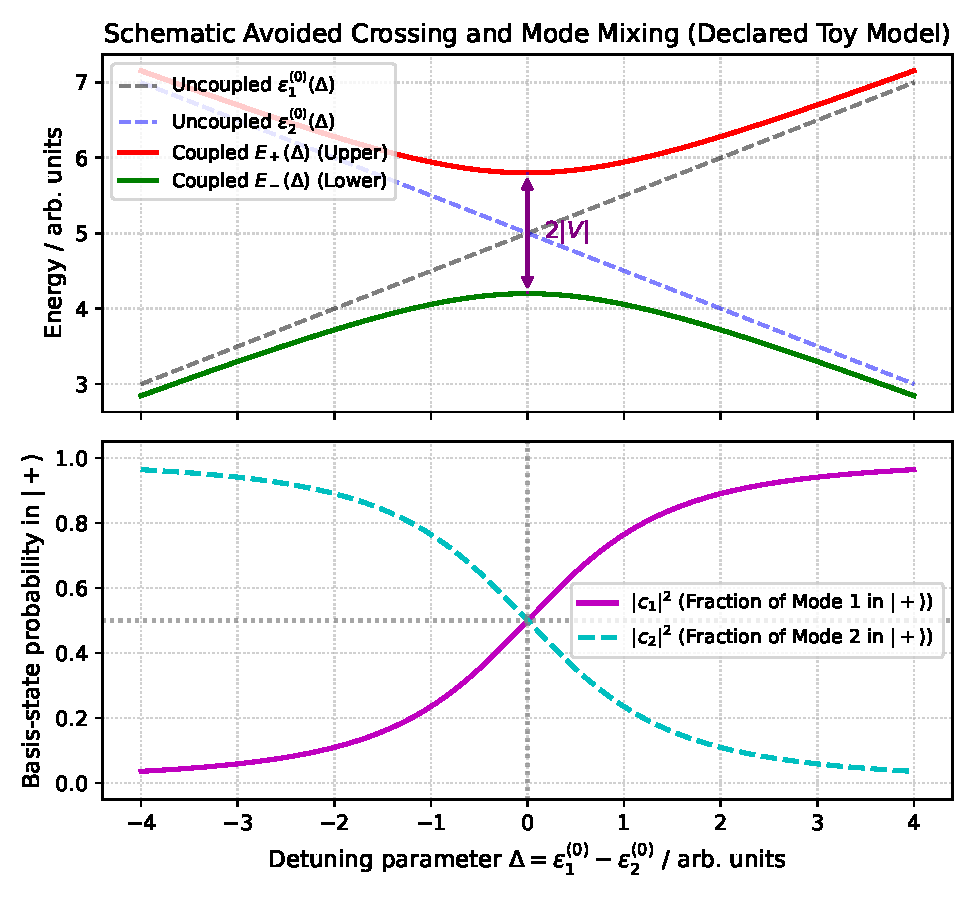
\includegraphics[width=0.95\textwidth]{Img/mode-mixing-avoided-crossing.pdf}
\caption[两态混合的避免交叉与基底概率]{声明参数两态量子混合教学模型中的避免交叉与基底成分权重交换示意图（输入脚本见附录F，采用教学参数 $V=0.8, \bar{\varepsilon}=5.0$ 任意单位）。(a) 未耦合能量本征值（虚线）与耦合后本征能量 $E_\pm(\Delta)$（实线），两支在失谐量 $\Delta = \varepsilon_1^{(0)} - \varepsilon_2^{(0)} = 0$ 处打开能隙 $2V$；(b) 上能级态 $|+\rangle$ 中原始基底 $|1\rangle$（实线）与基底 $|2\rangle$（虚线）的几率权重随失谐量的平滑过渡交换。图示展示的是独立的二态模型数学特性，不代表实核数据。}\label{fig:3-6-mode-mixing}
\end{figure}

联合预言判据包含以下四个相互联系的物理环节：
\begin{enumerate}
\item \textbf{能级避免交叉 (Avoided Crossing)}：随着控制参数改变，未耦合能级可以彼此逼近；在非零耦合作用下，本征能谱不相交。若 $V$ 固定且失谐量穿过零点，最小能隙为 $2V$（见图\ref{fig:3-6-mode-mixing}(a)）；若耦合也随自旋改变，最小间隔的位置和大小要由完整模型计算。
\item \textbf{波函数成分反转与重分布}：穿过避免交叉点前后，高能态与低能态中关于形状振动基底与取向摆动基底的几率成分发生连续交换（见图\ref{fig:3-6-mode-mixing}(b)）。
\item \textbf{电磁跃迁几率的相干干涉与重新分配}：由于电四极算符 $\mathcal{M}(E2)$ 对形状改变和转轴转动态具有不同的跃迁选择定则与矩阵元结构，两态的相干叠加将导致向末态 $|f\rangle$ 的折合跃迁几率展现出特征干涉效应：
\begin{equation}\label{eq:3-6-be2-interference}
B(E2; |+\rangle \to |f\rangle) = \frac{1}{2I_i + 1} \left| \cos\theta\,\langle f || \mathcal{M}(E2) || 1 \rangle + \sin\theta\,\langle f || \mathcal{M}(E2) || 2 \rangle \right|^2 ,
\end{equation}
其中双竖线代表 Wigner--Eckart 约化矩阵元，式前包含初态统计权因子 $\frac{1}{2I_i+1}$。令两个未混合矩阵元为 $M_1,M_2$，交叉项为 $2\cos\theta\sin\theta\,\operatorname{Re}(M_1M_2^*)$；它的大小与符号取决于振幅和相位，也可能为零。相干叠加本身不要求二态子空间覆盖整个希尔伯特空间。在这个固定算符、相同初态自旋的二态旋转中，向同一末态的两个 $B(E2)$ 之和保持不变；把这一性质推广到实核总强度时，还要检查被截去的态和变化的算符。
\item \textbf{多极混合比 $\delta(E2/M1)$ 的演化}：伴随着波函数成分从摆动取向主导向形状振动主导的平滑过渡，带间跨带跃迁的多极混合比 $\delta$ 的数值和符号取决于微观电四极与磁偶极矩阵元的相对相位与干涉效应，并不必然表现为单调显著的变化。
\end{enumerate}

必须强调：单凭实验测得的能级排斥或能级间隔突变，不能唯一确定存在形状模与取向模的耦合。在快转动核结构中，单粒子准粒子顺排（如回弯现象）、带交叉退耦或科里奥利反转均能在能谱上表现为能级排斥。因此，在实验数据分析中，必须严格区分直接谱学测量（能级与分支比）、唯象模型拟合与物理机制解释三层界限。

\subsection{微观自洽响应中旋转赝模的严格剔除}\label{sec:3-6-4}

当在微观准粒子随机相位近似（QRPA）或推转 RPA（CRPA）框架下研究高自旋激发态时，必须处理自发对称破缺引起的零频模问题。\cite{prochniak-rohozinski-2009-bohr-collective-hamiltonian,matsuzaki-2004-nuclear-inertia-and-wobbling}

在旋转参考系中，取推转算符 $\hat H'=\hat H-\omega_{\mathrm{rot}}\hat J_x$，其中 $\hat{\mathbf J}$ 具有作用量量纲，$\omega_{\mathrm{rot}}$ 为角频率。若全哈密顿量满足 $[\hat H,\hat J_k]=0$，角动量代数直接给出
\begin{equation}\label{eq:3-6-rotational-commutators}
[\hat H',\hat J_x]=0,\qquad
[\hat H',\hat J_y\pm i\hat J_z]
=\mp\hbar\omega_{\mathrm{rot}}(\hat J_y\pm i\hat J_z).
\end{equation}
这说明零频方向与推转频率处的转动赝模应区别对待，不能把所有低频解都认作新的形状或摆动激发。破缺平均场加RPA的实现需要检验相应的对称性恢复和赝模解耦。具体模型可以采用经过相容性校准的残余四极力等构造；二次拉伸相互作用是一些实现的选择，并非所有理论必须采用的唯一形式。\cite{matsuzaki-2004-nuclear-inertia-and-wobbling,kvasil-2006-dy156-yb162-crpa-wobbling} 若参考态、残余作用和截断空间不相容，赝模污染便可能影响所求的物理响应。

进一步，微观自洽线性响应导出的有效横向转动响应张量是在参考频率 $\omega_{\mathrm{rot}}$ 的自洽基底上，对小振幅微扰探针角频率 $\Omega$ 导出的动态响应导数：
\begin{equation}\label{eq:3-6-freq-dependent-inertia}
\chi_{kl}^{J\omega}(\Omega; \omega_{\mathrm{rot}}) = \left. \frac{\delta \langle \hat{J}_k \rangle(\Omega)}{\delta \omega_l(\Omega)} \right|_{\omega_{\mathrm{rot}}} .
\end{equation}
该张量依赖探针频率 $\Omega$ 与参考频率 $\omega_{\mathrm{rot}}$，其量纲为转动惯量。怎样从完整响应中构造摆动方程使用的有效横向惯量，取决于模型的约束及赝模处理，不能直接把任意单个张量元命名为通用的 $\mathcal J_\perp$。沿带动力学惯量 $\mathcal{J}^{(2)}=d\langle J_x\rangle/d\omega_{\mathrm{rot}}$ 描述物理角动量对沿带角频率的变化率；若改用无量纲 $I_x=\langle J_x\rangle/\hbar$，右侧需相应乘 $\hbar$。沿带变化与横向取向响应是不同问题。\cite{matsuzaki-2004-nuclear-inertia-and-wobbling}

\subsection{有限自旋非谐效应与局域声子标签边界}\label{sec:3-6-5}

在简谐多声子近似下，摆动带与 $\gamma$ 振动带通常被赋予离散的整数声子量子数 $n_{\mathrm{wob}} = 0, 1, 2, \dots$ 或 $n_\gamma = 0, 1, 2, \dots$。然而，在实际有限核体系中，这种简谐性只是局域展开下的渐近近似。

即使惯量固定，有限角动量也会限制局域声子展开：振幅增大或接近失稳点时，高阶角动量项可能不可忽略。在远离软模、固定低声子数的高自旋展开中，可按 $1/I$ 组织相对修正；这不是所有实核非谐性的统一数值定律。因此，不能把任意三条伴带直接指认为 $n=0,1,2$。不等间隔可能来自有限自旋运动学、准粒子顺排、形状极化或其它混合，需要比较各机制的联合预言。

\subsection{微观模型案例与核区观测边界}\label{sec:3-6-6}

为了审视真实核体系中形状模与取向模耦合的理论预言与实验现状，本小节梳理文献中代表性的微观计算与典型核区的观测边界。

\paragraph{1. TAC-HFB 框架下的高自旋摆动与 $\gamma$ 坐标探索}
Oi 与 Walker 选取 $^{164}\mathrm{Hf}$，用倾斜推转 HFB（TAC-HFB）沿取向角松弛内禀形状，再另设一维示意量子化讨论局域态及其混合。\cite{doctoral-r1-g37-oi-2001-wobbling-gamma-coupling} 这是把形状与取向联系起来的早期模型探索。其HFB空间未重现预期的TSD形变；一维量子化的边界和质量参数也含另外的假设，不能视为完整的微观集体哈密顿量或实验能带。原文以 $a=M_w\omega^2/2$ 定义势能系数后给出的质量关系，还存在反解应保留因子2的代数疑点。这是对原式的一致性核查，尚不足以替代完整模型复算。S/A等局域标记也不应被改称为守恒的实验室空间宇称。

\paragraph{2. 推转 HFB+CRPA 框架下的配对与对顺排响应}
Kvasil 与 Nazmitdinov 用指定的推转 Nilsson 加RPA框架比较 $^{156}\mathrm{Dy}$ 与 $^{162}\mathrm{Yb}$，在模型内将两核的带弯曲分别联系到 $\gamma$ 软化和中子对顺排，并讨论Dy的奇自旋 $\gamma$ 分支向摆动型激发的演化。\cite{kvasil-2006-dy156-yb162-crpa-wobbling} 其配对隙在带交叉附近采用唯象处方；因而“自洽响应”不意味着所有输入均由同一个无近似理论确定。惯量和带间E2/M1的共同比较提供了区分机制的途径，这些仍是该模型范围内的解释。

\paragraph{3. 三轴投影壳模型（TPSM）在偶偶核中的应用与限制}
Bhat 等人用三轴投影壳模型（TPSM），在包含真空、两准粒子及四准粒子构型的截断空间中进行三维角动量投影，比较 $^{76}\mathrm{Ge}, ^{112}\mathrm{Ru}, ^{188,192}\mathrm{Os}, ^{192}\mathrm{Pt}, ^{232}\mathrm{Th}$。\cite{doctoral-r1-g37-bhat-2025-microscopic-wobbling-even-even} 作者结合组态顺排与计算的电磁性质，将其中五个案例解释为摆动型激发，保留 $^{232}\mathrm{Th}$ 为反例。这不等于六核均已获实验确证。轴向形变采用参考输入，非轴形变以再现 $\gamma$ 带头为目标选取，部分配对输入也有调整；拟合所用能量不能再次当作独立验证。需要由寿命、带间电磁强度及其它未参与调参的观测检验这些解释。

形状与取向自由度可以耦合；近简并会放大给定非零相互作用造成的混合，频率不接近也不意味着耦合项必为零。能级排斥只显示相容态间的作用，不能独自辨认被混合的自由度。实际研究应先给出所选模型的能谱、跃迁及响应联合预言，再用未参与调参的资料比较它与准粒子顺排等竞争机制；若现有观测仍不足以区分，就保留这一解释边界。
%
}{%
    \section{$\gamma$形状模与取向模的耦合 [未完成]}\label{sec:3-6}%
    \textit{本节尚未完成。}%
}

%-- Section 3.7: 八极与反射不对称的联立问题
\setcounter{section}{6}%
\IfFileExists{Tex/Sections/sec-3-7.tex}{%
    \section{八极与反射不对称的联立问题}\label{sec:3-7}

在第\ref{sec:3-5}节中，我们探讨了原子核在四极三轴形变背景下，由多体角动量在内禀空间发生非共面矢量耦合所诱发的集体转动手征对称性自发破缺；在第\ref{sec:2-5}节与第\ref{sec:3-1}节中，阐明了有限多体系统连续转动对称性与分立空间反演的守恒本质与量子波包投影恢复机制。然而，在某些特定的核区（如轻稀土钡铈区、重锕系区以及 $A \approx 70$--$80$ 质量区），原子核不仅展现出非轴对称四极形变，而且费米面附近存在由宇称相反且角动量相差三个单位（$\Delta l = 3, \Delta j = 3$）的单粒子轨道对所激发的八极关联（Octupole correlations）。当空间反射不对称的梨形八极形变与手征非共面三轴转动在同一核结构中同时出现时，体系的对称性破缺与恢复展现出更为复杂的拓扑图像。

在在束 $\gamma$ 谱学分析中，不能简单将两种独立的物理现象直观相加，误认为只要在伴带间观察到微弱的 $E1$ 跃迁连接以及四条表观近简并的能带，便必然意味着原子核实现了手征对称性与空间反射对称性的联立自发破缺。本节旨在严格厘清八极形变与三次四极不变量 $q_3$ 的算符界限、分析标量三重积在空间反演、时间反演与正交空间反射下的本质变换特性，剖析线性幺正宇称投影与反幺正手征操作的代数对立，解析微观八极驱动机制与软核竞争，并深入探讨电偶极矩 $|D_0|$ 提取的模型假定与综合实验判定准则。

\subsection{八极算符、反演破坏与四极三次不变量的区别}\label{sec:3-7-1}

在探讨八极物理之前，首先必须建立算符阶数与张量性质的严格界限，防止符号与物理对象的混淆：
\begin{enumerate}
\item \textbf{八极自由度的算符阶数与物理量纲}：八极形变描述原子核质量或电荷分布的梨形或反射不对称畸变，由三阶球张量坐标 $\alpha_{3\mu}$（$\mu = -3, \dots, +3$）或形变度 $\beta_3$ 描述。相应的电磁跃迁算符为电八极算符 $\hat{\mathcal{M}}(E3, \mu)$，它是具有负宇称的 3 阶球张量算符（在空间反演下变号：$\hat{\Pi} \hat{\mathcal{M}}(E3) \hat{\Pi}^{-1} = -\hat{\mathcal{M}}(E3)$），其电磁跃迁几率 $B(E3)$ 具有量纲 $e^2\cdot\mathrm{fm}^6$；
\item \textbf{四极三次不变量 $q_3$ 的算符身份与量纲}：在全篇论文（特别是在第\ref{sec:2-1}节与第\ref{sec:2-4}节）中，$q_3$ 严格代表由二阶电四极算符张量缩并构成的标量三次不变量：
\begin{equation}\label{eq:3-7-q3-def}
q_3 \equiv -\sqrt{\frac{7}{2}} \langle (\hat{Q}_2 \times \hat{Q}_2)_2 \cdot \hat{Q}_2 \rangle = \langle Q^3 \cos(3\gamma) \rangle,
\end{equation}
右端是相应 Bohr 电四极坐标映射下的记法，不要求存在唯一经典形状或固定 $\gamma$。其算符定义在张量阶数上为 rank-0 标量不变量，电荷长度量纲为 $e^3\cdot\mathrm{fm}^6$，绝非能量量纲。$q_3$ 描述的是纯四极形变下的三轴不对称度（$\gamma$ 偏离），本身具有正宇称，绝非八极可观测量。但必须澄清，算符类型与张量阶数的区别并不意味着四极与八极自由度在实际多体动力学上绝对无关，亦不要求体系的八极形变 $\beta_3 = 0$；在四极—八极耦合态中，波函数在八极关联下的重构同样会引起 $q_3$ 期望值的动力学演化。此处严格规范的，是禁止将四极不变量符号 $q_3$ 借用于指代八极形变度 $\beta_3$ 或八极跃迁 $B(E3)$；
\item \textbf{内禀反演破坏与实验室良宇称定态}：在内禀体轴参考系中，若存在静态反射不对称形变（$\beta_3 \ne 0$），核密度分布破坏空间反演不变性（$\rho(-\mathbf{r}) \ne \rho(\mathbf{r})$）。然而在没有外场作用的孤立原子核中，强相互作用与电磁相互作用哈密顿量满足空间反演守恒：
\begin{equation}\label{eq:3-7-H-parity-commute}
[\hat{H}, \hat{\Pi}] = 0.
\end{equation}
实验室系中的物理定态本征态具有确定的良空间宇称 $\pi = \pm 1$。根据宇称选择定则，任何奇宇称不可约张量算符在同宇称定态之间的对角期望值严格为零：
\begin{equation}\label{eq:3-7-E3-diag-zero}
\langle \pi | \hat{\mathcal{M}}(E3, 0) | \pi \rangle \equiv 0.
\end{equation}
因此，在上述良宇称实验室定态中，电八极算符的静态期望值为零。八极关联的实验约束来自相反宇称态之间的 $E3$ 矩阵元及相关谱结构；增强的单个或分布式八极强度、八极振动与交替宇称转动带可以提供不同层次的信息。将这些量映射为内禀静态 $\beta_3$ 仍需说明模型与波函数条件。
\end{enumerate}

\subsection{标量三重积在空间反演、时间反演与正交反射下的变换性质}\label{sec:3-7-2}

手征对称性自发破缺的核心标志，是在旋转参考系下由质子准粒子角动量 $\mathbf{j}_p$、中子准粒子角动量 $\mathbf{j}_n$ 以及核芯集体转动角动量 $\mathbf{R}$ 构成的非共面三面角结构。标量三重积表征了该三面角的手征旋向性：
\begin{equation}\label{eq:3-7-triple-product}
\chi_{\text{geom}} \equiv \mathbf{j}_p \cdot (\mathbf{j}_n \times \mathbf{R}).
\end{equation}

考察基本物理矢量在空间反演算符 $\hat{\Pi}$、反幺正时间反演算符 $\mathcal{T}$ 以及普通空间平面反射下的变换行为：
\begin{enumerate}
\item \textbf{量子算符厄米性与独立张量空间}：若将 $\mathbf{j}_p, \mathbf{j}_n, \mathbf{R}$ 视为分别作用于质子准粒子、中子准粒子与集体核芯不同希尔伯特子空间的独立张量因子，由于不同子空间的算符彼此对易（$[\mathbf{j}_p, \mathbf{j}_n] = 0, [\mathbf{j}_p, \mathbf{R}] = 0, [\mathbf{j}_n, \mathbf{R}] = 0$），标量三重积算符 $\hat{\chi}_{\text{geom}} = \epsilon_{ijk} \hat{j}_{p,i} \hat{j}_{n,j} \hat{R}_k$ 自身已天然具备严格的厄米性（$\hat{\chi}_{\text{geom}}^\dagger = \hat{\chi}_{\text{geom}}$），无需人为施加跨空间对易对称化；
\item \textbf{空间反演 $\hat{\Pi}$ 下的轴矢量行为}：坐标与动量是极矢量（满足 $\hat{\Pi} \mathbf{r} \hat{\Pi}^{-1} = -\mathbf{r}$ 与 $\hat{\Pi} \mathbf{p} \hat{\Pi}^{-1} = -\mathbf{p}$）。然而角动量是由两者叉乘定义的轴矢量（伪矢量）：
\begin{equation}\label{eq:3-7-L-parity}
\hat{\Pi} \hat{\mathbf{J}} \hat{\Pi}^{-1} = \hat{\Pi} (\mathbf{r} \times \mathbf{p}) \hat{\Pi}^{-1} = (-\mathbf{r}) \times (-\mathbf{p}) = + \hat{\mathbf{J}}.
\end{equation}
由于体系内部全部角动量分量（无论是轨道角动量还是内禀自旋）在空间反演下均不改变方向：
\begin{equation}\label{eq:3-7-components-parity}
\hat{\Pi} \mathbf{j}_p \hat{\Pi}^{-1} = +\mathbf{j}_p, \quad \hat{\Pi} \mathbf{j}_n \hat{\Pi}^{-1} = +\mathbf{j}_n, \quad \hat{\Pi} \mathbf{R} \hat{\Pi}^{-1} = +\mathbf{R}.
\end{equation}
代入标量三重积算符得到：
\begin{equation}\label{eq:3-7-triple-parity-invariance}
\hat{\Pi} \left[ \mathbf{j}_p \cdot (\mathbf{j}_n \times \mathbf{R}) \right] \hat{\Pi}^{-1} = (+\mathbf{j}_p) \cdot \left[ (+\mathbf{j}_n) \times (+\mathbf{R}) \right] = + \mathbf{j}_p \cdot (\mathbf{j}_n \times \mathbf{R}).
\end{equation}
式~\eqref{eq:3-7-triple-parity-invariance} 表明：角动量标量三重积是严格的空间反演偶标量（$\mathcal{P}$ 偶），空间反演自身绝对不能反转转动体系的手征旋向；
\item \textbf{普通空间平面正交反射下的不变性及其物理内涵}：考察空间中任意平面的正交镜像反射（设为关于 $xy$ 平面的反射 $\sigma_z: z \to -z$）。极矢量在 $\sigma_z$ 下满足 $(x, y, z) \to (x, y, -z)$；然而根据轴矢量定义 $\mathbf{J} = \mathbf{r} \times \mathbf{p}$，轴矢量的变换矩阵为：
\begin{equation}\label{eq:3-7-axial-reflection}
J_x \to -J_x, \quad J_y \to -J_y, \quad J_z \to +J_z \implies M_{\text{axial}} = \begin{pmatrix} -1 & 0 & 0 \\ 0 & -1 & 0 \\ 0 & 0 & 1 \end{pmatrix}.
\end{equation}
矩阵 $M_{\text{axial}}$ 的行列式为 $\det(M_{\text{axial}}) = (-1) \times (-1) \times (+1) = +1$。因此三个轴矢量的标量三重积在普通空间平面的镜像反射下严格保持不变：
\begin{equation}\label{eq:3-7-reflection-preserve}
\det[M_{\text{axial}}\mathbf{j}_p, M_{\text{axial}}\mathbf{j}_n, M_{\text{axial}}\mathbf{R}] = \det(M_{\text{axial}}) \det[\mathbf{j}_p, \mathbf{j}_n, \mathbf{R}] = +\mathbf{j}_p \cdot (\mathbf{j}_n \times \mathbf{R}).
\end{equation}
式~\eqref{eq:3-7-reflection-preserve} 证明：普通空间平面正交反射并不反转标量三重积 $\chi_{\text{geom}}$，因而该手征旋向性并非空间宇称奇（$\mathcal{P}$ 奇）的序参量。必须明确指出，标量积本身在反射下的不变性并不等同于整个取向核态或三矢量空间构型在普通空间反射下完全不变；
\item \textbf{时间反演 $\mathcal{T}$ 下的反转行为与标准手征算符}：时间反演算符反转运动方向与自旋（$\mathcal{T} \hat{\mathbf{J}} \mathcal{T}^{-1} = -\hat{\mathbf{J}}$）：
\begin{equation}\label{eq:3-7-triple-time-reversal}
\mathcal{T} \left[ \mathbf{j}_p \cdot (\mathbf{j}_n \times \mathbf{R}) \right] \mathcal{T}^{-1} = (-\mathbf{j}_p) \cdot \left[ (-\mathbf{j}_n) \times (-\mathbf{R}) \right] = - \mathbf{j}_p \cdot (\mathbf{j}_n \times \mathbf{R}).
\end{equation}
时间反演 $\mathcal{T}$ 单独即可反转标量三重积（$\mathcal{T}$ 奇）。在体轴参考系中，引入复合算符 $\mathcal{C} = \mathcal{T} \mathcal{R}_y(\pi)$ 提供了实现单一内禀分量反转的标准且便捷的物理操作，但它并非实现符号反转的唯一可能数学变换。
\end{enumerate}

\subsection{反幺正手征算符 $\mathcal{C}$、空间宇称 $\hat{\Pi}$ 与态恢复}\label{sec:3-7-3}

当原子核在微观自洽平均场中同时出现空间反射不对称（$\beta_3 \ne 0$）与非共面手征转动时，体系展现出两套离散对称性的自发破缺：
\begin{itemize}
\item 空间反射对称性破缺：由正负八极形变态 $|\Phi(+\beta_3)\rangle$ 与反演态 $|\Phi(-\beta_3)\rangle = \hat{\Pi} |\Phi(+\beta_3)\rangle$ 关联；
\item 手征转动对称性破缺：由左手三面角态 $|L\rangle$ 与右手态 $|R\rangle = \mathcal{C} |L\rangle$ 关联，标准手征算符为 $\mathcal{C} \equiv \mathcal{T} \mathcal{R}_y(\pi)$。
\end{itemize}

在此必须深入考察线性算符 $\hat{\Pi}$ 与反幺正算符 $\mathcal{C}$ 在复希尔伯特空间中的代数对立：
\begin{enumerate}
\item \textbf{标准手征算符的反幺正本质与相作用}：算符 $\mathcal{C} = \mathcal{T} \mathcal{R}_y(\pi)$ 作用在内禀体轴角动量分量上，由于 $\mathcal{R}_y(\pi)$ 将 $(J_1, J_2, J_3) \to (-J_1, J_2, -J_3)$，而时间反演将所有分量变号，二者复合的作用等效于单一内禀分量的符号翻转：
\begin{equation}\label{eq:3-7-C-action}
J_1 \to +J_1, \quad J_2 \to -J_2, \quad J_3 \to +J_3.
\end{equation}
由于时间反演 $\mathcal{T}$ 为反线性算符，$\mathcal{C}$ 是严格的反幺正算符。反幺正算符的本征值方程 $\mathcal{C}|\psi\rangle = \lambda |\psi\rangle$ 在全域定相变换 $|\psi'\rangle = e^{i\phi}|\psi\rangle$ 下变为 $\lambda' = e^{-2i\phi}\lambda$，其相位敏感依赖于波函数规范，不能像线性幺正算符那样定义规范不变的实数本征量子数；因此 $\mathcal{C}$ 绝不能充当类似空间宇称的 $\pm 1$ 手征宇称标签；
\item \textbf{$\mathcal{C}^2 = +1$ 代数与二重简并条件}：对于整数总自旋（偶费米子数）体系，时间反演与 $\pi$ 旋转算符均满足 $\mathcal{T}^2 = +1$ 且 $\mathcal{R}_y(\pi)^2 = +1$；对于半整数总自旋（奇费米子数）体系，二者均满足 $\mathcal{T}^2 = -1$ 且 $\mathcal{R}_y(\pi)^2 = -1$。由于时间反演算符与空间旋转算符对易，在任一自旋情形下算符模方严格满足：
\begin{equation}\label{eq:3-7-C-square}
\mathcal{C}^2 = \mathcal{T} \mathcal{R}_y(\pi) \mathcal{T} \mathcal{R}_y(\pi) = \mathcal{T}^2 \mathcal{R}_y(\pi)^2 = (-1)^{2I} (-1)^{2I} = (-1)^{4I} = +1.
\end{equation}
由于 $\mathcal{C}^2 = +1$ 而非反幺正克喇默斯算符的 $-1$，该手征反转算符 $\mathcal{C}$ 自身并不提供克喇默斯定理强制的二重能级简并保护（但不排除微观体系中由其他独立对称性所带来的可能简并）；
\item \textbf{几何势阱耦合与宇称投影的物理边界}：在多维形变与取向空间中，空间反射自由度（$\beta_3$）与转动取向自由度在动力学势能面上发生非线性耦合，体系并不必然在所有核中都演化出四个孤立且互不连通的物理势阱。线性幺正宇称投影算符 $P^\pm = (\hat{\mathbf{1}} \pm \hat{\Pi})/2$ 划分出的正宇称与负宇称子空间严格正交（$P^+ P^- = 0$；此时尽管底层的内禀波包 $|\Phi(\pm\beta_3)\rangle$ 存在非正交重叠，但投影后的态矢属于正交子空间）。然而，宇称投影自身绝不保证正负宇称带之间的能级近简并；正宇称子空间内的手征劈裂 $\Delta E^+$ 与负宇称子空间内的手征劈裂 $\Delta E^-$ 受控于各自势阱内的动力学势垒与量子隧穿重叠，在数值上通常不相等。因此，在实验谱学中，四条相互平行的能带绝非无条件的数学定理，亦不能仅凭能谱存在四条邻近能带便孤立判定体系实现了手征与八极的联立自发破缺。
\end{enumerate}

\subsection{微观八极关联驱动机制：壳结构与轨道对}\label{sec:3-7-4}

微观核多体理论揭示了内禀八极形变与八极关联产生的本质驱动力。八极单粒子势场 $\hat{V}_{\text{oct}} \propto r^3 Y_{3\mu}$ 属于奇宇称算符，其非零单粒子矩阵元只能发生在宇称相反且轨道角动量相差奇数单位的单粒子态之间。

根据电八极算符的角动量三角不等式 $|j_1 - j_2| \le 3 \le j_1 + j_2$ 以及宇称选择定则（要求轨道角动量差 $\Delta l = l_1 - l_2$ 必为奇数），单粒子态之间跃迁允许出现：
\begin{equation}\label{eq:3-7-delta-lj}
\Delta l = 1, 3, \quad \Delta j \le 3.
\end{equation}
其中，由离心势能与自旋—轨道分裂驱动的最强相干驱动组合，常见于满足如下选择条件的轨道对：
\begin{equation}\label{eq:3-7-favored-octupole}
\Delta l = 3, \quad \Delta j = 3.
\end{equation}
需要明确指出：$\Delta l = 3, \Delta j = 3$ 是提供强八极矩阵元相干放大的优势物理机制，但并非发生八极激发的严格数学充分必要条件。式~\eqref{eq:3-7-delta-lj} 允许的 $\Delta l = 1$ 单粒子跃迁同样对总八极响应提供背景贡献。

不同核区的微观驱动轨道对由壳层能级排布严格决定（Butler 与 Nazarewicz 1996）~\cite{butler-nazarewicz-1996-intrinsic-reflection-asymmetry}：
\begin{itemize}
\item 在轻稀土八极核区（如 $^{144, 146}\mathrm{Ba}$，质子数 $Z \approx 56$，中子数 $N \approx 88$），质子费米面靠近 $d_{5/2} \leftrightarrow h_{11/2}$ 轨道对（$l = 2 \leftrightarrow 5, j = 5/2 \leftrightarrow 11/2$），中子费米面靠近 $f_{7/2} \leftrightarrow i_{13/2}$ 轨道对（$l = 3 \leftrightarrow 6, j = 7/2 \leftrightarrow 13/2$）；
\item 在重核与锕系八极强形变区（如 $^{224}\mathrm{Ra}$，质子数 $Z = 88$，中子数 $N = 136$，处于 $N \approx 134$ 强八极驱动区），质子费米面由 $f_{7/2} \leftrightarrow i_{13/2}$ 轨道对主导，中子费米面由 $g_{9/2} \leftrightarrow j_{15/2}$ 轨道对（$l = 4 \leftrightarrow 7, j = 9/2 \leftrightarrow 15/2$）主导。绝不能将轻稀土区的钡同位素单粒子轨道对套用到锕系镭同位素上；
\item 在中等质量核区（$A \approx 70$--$80$，如 $^{78}\mathrm{Br}, ^{74}\mathrm{As}$），费米面附近存在质子或中子的 $p_{3/2}$ 与侵入轨道 $g_{9/2}$ 对（$l = 1 \leftrightarrow 4, j = 3/2 \leftrightarrow 9/2$）~\cite{liu-chen-2016-78br-chirality-reflection-symmetry-thesis,xiao-xiao-2019-high-spin-74as-thesis}。
\end{itemize}

在微观分析中必须恪守物理边界：费米面附近具备 $\Delta l = \Delta j = 3$ 轨道对仅是提供八极相干吸引的动力学驱动，原子核是否能够在势能面上形成深陷且稳定的静态八极极小（$\beta_3 \ne 0$），取决于该相互作用能否压倒四极形变刚度以及单粒子动能恢复力。在许多核素中，势能面呈现出沿 $\beta_3$ 极其平缓的八极软势或以 $\beta_3=0$ 为中心的简谐势阱，此时体系展现出强烈的八极表面动态振动（Octupole vibrations），而非刚性静态梨形反射不对称。

\subsection{电偶极矩 $|D_0|$ 提取模型假设与综合实验判定准则}\label{sec:3-7-5}

在实验谱学中，连接相反宇称伙伴带的核心电磁跃迁是电偶极跃迁（$E1$）。然而，从实验观测到的 $E1$ 跃迁强度反演微观八极形变，包含着一系列强烈的理论模型假设。

\subsubsection{内禀电偶极矩 $D_0$ 的产生机制与反常相消}

在宏观均匀带电的刚体椭球中，质心与电荷中心完全重合，不存在内禀静态电偶极矩（$D_0 \equiv 0$）。当核发生反射不对称八极形变时，在唯象宏观液滴与微观单粒子极化两分法下，内禀电偶极矩可表示为：
\begin{equation}\label{eq:3-7-D0-components}
D_0 = D_0^{\text{macro}} + D_0^{\text{micro}}.
\end{equation}
需要特别指出，式~\eqref{eq:3-7-D0-components} 属于一种唯象的宏观液滴位移与微观单粒子壳修正的分解约定，不能假设两项在所有核区均普遍符号相反。

在特定核素中，微观壳层结构的变化可能引发剧烈的电偶极矩压低。例如在 $^{146}\mathrm{Ba}$ 的直接库仑激发实验中（Bucher 等人 2017）~\cite{bucher-2017-146ba-direct-octupole}，多步 Coulomb 激发实验直接测定的是基态电八极跃迁矩阵元 $|\langle 3_1^- || \hat{\mathcal{M}}(E3) || 0_1^+ \rangle| = 0.65_{-0.20}^{+0.14} \, e\cdot\mathrm{b}^{3/2}$，对应跃迁强度 $B(E3; 3_1^- \to 0_1^+) = 48_{-29}^{+21} \, \mathrm{W.u.}$（Bucher 等人 2017 原文表 I 与图 3--5）。该直接测量确立了 $^{146}\mathrm{Ba}$ 具有与 $^{144}\mathrm{Ba}$ 相当的强八极集体性。文献中所列出的 $E1$ 跃迁矩阵元约束主要沿用既有的平均寿命与光子分支比数据，而非该次库仑激发直接独立产出。在 Bucher 等人（2017）引用的自洽对称性守恒组态混合（SCCM，Gogny D1S）计算中，对同位素内禀偶极矩演化的微观解释，具体归因于质子与中子各自对内禀偶极贡献的对比——特别是费米面附近中子高 $j$、低 $K$ 侵入轨道占据的演化调控了总偶极矩的抵消与变号，这与宏观/微观唯象两分法属于不同维度的物理描述。强八极跃迁强度与微弱 $E1$ 跃迁并存的现象表明：微弱的 $E1$ 跃迁并不意味着八极集体性的消失；反之，强 $E1$ 跃迁亦不能孤立证明静态刚性梨形形变的存在（强 $E3$ 自身亦包含八极动态振动的物理可能）。

\subsubsection{转子模型提取 $|D_0|$ 的假设前提与多极混合界限}

在强耦合单 $K$ 轴对称转子模型假定下，相反宇称带之间的带间 $B(E1)$ 跃迁几率与同带内 $B(E2)$ 满足 Clebsch--Gordan 几何偶合关系：
\begin{equation}\label{eq:3-7-BE1-axial-formula}
B(E1; I \to I-1) = \frac{3}{4\pi} D_0^2 \, \langle I \, K \, 1 \, 0 | I-1 \, K \rangle^2,
\end{equation}
\begin{equation}\label{eq:3-7-BE2-axial-formula}
B(E2; I \to I-2) = \frac{5}{16\pi} Q_0^2 \, \langle I \, K \, 2 \, 0 | I-2 \, K \rangle^2.
\end{equation}
两者的比值给出：
\begin{equation}\label{eq:3-7-D0-Q0-ratio}
\frac{B(E1; I \to I-1)}{B(E2; I \to I-2)} = \frac{12}{5} \frac{D_0^2}{Q_0^2} \frac{\langle I \, K \, 1 \, 0 | I-1 \, K \rangle^2}{\langle I \, K \, 2 \, 0 | I-2 \, K \rangle^2}.
\end{equation}
在 $K=0$ 的交替宇称带中，Clebsch--Gordan 符号之比化简为 $\frac{\langle I 0 1 0 | I-1 0 \rangle^2}{\langle I 0 2 0 | I-2 0 \rangle^2} = \frac{2(2I-1)}{3(I-1)}$，与 $12/5$ 相乘给出化简式 $\frac{B(E1)}{B(E2)} = \frac{8}{5} \left( \frac{2I-1}{I-1} \right) \frac{D_0^2}{Q_0^2}$；文献中常见的 $8/5$ 前因子仅在该 $K=0$ 显式代数化简后成立，保留未化简 CG 比时前因子严格为 $12/5$。

审视式~\eqref{eq:3-7-D0-Q0-ratio} 的物理前提与实验推断边界：
\begin{itemize}
\item \textbf{强耦合单 $K$ 条件}：该式严格假定核具有稳定的单轴转动态且投影量子数 $K$ 良好守恒。在三轴变形核或存在强烈 $K$ 混合的核中，电偶极算符在内禀系存在多个非零分量（如横向分量 $D_1$），不能通过单一分支简化为单一标量 $D_0$；
\item \textbf{四极矩输入与比值确定性}：若实验仅测得退激光子分支比，在缺乏能级寿命测量且无 Coulomb 激发等绝对跃迁矩阵元数据时，公式只能导出比值 $|D_0 / Q_0|$。若要提取绝对内禀偶极矩 $|D_0|$，可结合同核已独立测定的内禀四极矩 $Q_0$（由同核带内 $B(E2)$ 或跃迁四极矩 $Q_t$ 导出），或在缺乏实验数据时结合微观模型自洽映射的 $Q_0$；若已取得绝对 $B(E1)$，也可直接由式~\eqref{eq:3-7-BE1-axial-formula}求 $|D_0|$，不必先定 $Q_0$。该比值仅含偶极矩模方，不能确定 $D_0$ 的物理符号；
\item \textbf{多极混合与谱线重叠的严格区分}：在连接相反宇称能级的同一物理跃迁内部，电磁相互作用的宇称守恒律（要求多极辐射具有负宇称 $\Delta \pi = -1$）在初末自旋同时允许 $L=1,2$ 的低阶截断下，可发生 $E1 + M2$ 多极混合（其中 $E1$ 为电偶极，$M2$ 为磁四极），其多极混合比 $\delta(M2/E1)$ 可通过角分布与偏振测量进行实验反演。必须严格区分这一物理多极混合与谱学中的偶然能谱重叠现象（即一条连接相反宇称能级的 $E1$ 跃迁谱线，与另一条连接同宇称能级的 $M1$ 或 $E2$ 跃迁谱线在探测器能量分辨率窗口内偶然发生能量重叠组成的实验 doublet），严禁在物理上断言单一跃迁内部能出现 $E1 + M1$ 或 $E1 + E2$ 混合。
\end{itemize}

\subsubsection{多维实验观测量与模型前向检验准则}

为了在实验上客观甄别手征与空间反射对称性的联立动力学特征，低能核结构谱学确立了联合多维实验可观测量、对比理论模型前向预言的综合分析准则：
\begin{enumerate}
\item \textbf{能谱四重结构对账}：检验理论模型是否能自洽预测自旋宇称序列为 $(I^+, I^-)$ 与伙伴带 $(I'^+, I'^-)$ 的四条相互平行的转动序列；
\item \textbf{电磁跃迁网络的实验约束}：
\begin{itemize}
\item 带内展现出同宇称 $\Delta I = 2$ 电四极跃迁（反映四极集体转动核心）；
\item 同宇称伙伴带之间展现出特征性的 $\Delta I = 1$ 的 $M1$ 与 $E2$ 连接跃迁（反映三维手征转动动力学）；
\item 相反宇称伙伴带之间展现出交错 $\Delta I = 1$ 的电偶极 $E1$ 连接跃迁（反映空间反射不对称或八极相干关联）；
\end{itemize}
\item \textbf{八极集体性与绝对跃迁几率约束}：强 $E1$ 跃迁并不等价于八极集体性，$E3$ 具有独立的动力学起源；应尽可能通过 Coulomb 激发或能级寿命测定获取绝对跃迁几率 $B(E2)$、$B(M1)$ 与关键的电八极跃迁强度 $B(E3)$；
\item \textbf{自洽微观模型的前向预言检验}：最终判定必须依据具体选定的理论模型（如约束反射不对称协变密度泛函理论、三维粒子—转子模型 RAT-PRM 或投影微观计算），在统一参数下对比能谱能级差、电磁跃迁分支比与四极/八极形变势能曲面的柔软度。不应将特定唯象框架下的所有理论连接项列为跨模型通用的排他性绝对认证清单。
\end{enumerate}

必须指出：在中等质量核区（如 $^{78}\mathrm{Br}, ^{74}\mathrm{As}$），实验已报道了包含同宇称与相反宇称带间跃迁的候选能级图景（Liu 等人 2016，Liu 2016，Xiao 2019）~\cite{liu-2016-octupole-correlations-multiple-chiral-doublet-bands-78br,liu-chen-2016-78br-chirality-reflection-symmetry-thesis,xiao-xiao-2019-high-spin-74as-thesis}。然而由于关键态能级寿命与绝对跃迁强度的实验测量精度限制，以及单粒子能级交叉与微观八极软势涨落的强烈竞争，在本节比较的所引资料和模型范围内，这些结构支持手征与八极关联的候选解释，尚不足以排他地确立刚性四重态。关于具体核素的详细实验数据、分支比矩阵与微观泛函势能面的定量对账，将在第\ref{sec:4-5}节中展开深入的专题比较。
%
}{%
    \section{八极与反射不对称的联立问题 [未完成]}\label{sec:3-7}%
    \textit{本节尚未完成。}%
}

%-- Section 3.8: 模式判断需要怎样的联合预言
\setcounter{section}{7}%
\IfFileExists{Tex/Sections/sec-3-8.tex}{%
    \section{模式判断需要怎样的联合预言}\label{sec:3-8}

在低能核结构高自旋谱学研究中，研究者常常依据个别能级比值接近某种理想转子或振子规律，或依据观测到一条相对增强的带间跃迁，便赋予实验能带特定的模式标签（如“手征双重带”、“横向摆动带”或“八极反射不对称带”）。然而，正如第\ref{chap:2}章第\ref{sec:2-8}节的综合比较所指出的，不同物理模型由于包含若干可调参数，在低激发能区往往表现出显著的拟合简并。若仅凭能谱局域拟合便断言某种运动模式已确立，容易将参数自由度带来的数值符合误认为物理机制的确证。

为了克服这一局限，本节旨在探讨如何将模式候选转化为具有明确前向预言、最强替代解释和判决性检验路径的研究问题：首先梳理理论模型的前向预言架构与参数输入；进而分析竞争解释在低能区的参数重叠与不可通约性，明确为何不能设立通用的唯象绝对阈值；接着建立包含误差协方差的数据分层架构与留出检验准则；最后基于已有文献原件基线，提出三个具体可证伪的实证研究候选方案（$^{98}\mathrm{Mo}$ 弱跨带电八极跃迁候选、$^{102}\mathrm{Ru}$ 低能偶极响应聚集与 $A \approx 130$ 低自旋取向进动），为后续全书跨质量区实测分析与实验统计反演提供方法论参照。\cite{lawrie-2020-tilted-precession-wobbling,frauendorf-2014-transverse-wobbling,nomura-2022-questioning-wobbling-ibfm,lv-2022-evidence-against-wobbling-135pr,matta-2015-transverse-wobbling-135pr,karmakar-2026-98mo-octupole,saracino-2026-102ru-scissors-octupole-resonances}

\subsection{模式的前向预言结构与模型空间划分}\label{sec:3-8-1}

一个自洽的核结构物理模型，不是事后对实验能级的唯象拟合公式，而是基于明确物理假定对多维物理量的前向映射系统。无论采用全微观自洽理论还是具有明确假定的唯象有效模型，建立一个模式的前向理论预言，均须明确以下四个核心要素：
\begin{enumerate}
\item \textbf{选定的动力学自由度划分}：明确模型保留的主导动力学变量（如转动欧拉角取向坐标、玻尔四极形状坐标 $\beta, \gamma$ 或特定单粒子轨道准粒子算符），以及被冻结或消去的自由度（如高能虚激发或高阶多极形变）。
\item \textbf{守恒量子数与对称性约束}：明确态波函数具有的确定总角动量与宇称 $I^\pi$，以及所保持的离散对称性（如绕内禀主轴旋转 $\pi$ 的签名量子数）。需要特别强调：时间反演 $\hat{\mathcal{T}}$ 是反幺正算符（包含复共轭变换 $i \to -i$），它并不具备普通的线性幺正本征值（不能赋予简单的标量 $\pm 1$ 标签），其动力学约束体现为半整数费米子系统的克喇末简并（$\hat{\mathcal{T}}^2 = -1$）、哈密顿量的时间反演不变性以及电磁跃迁基矢间的确定相位关联。
\item \textbf{势能面与动力学输入}：明确底层势能曲面、转动惯量张量 $\mathcal{J}_k(\omega)$、微观对能隙 $\Delta$ 以及有效跃迁算符。需要指出，具有明确物理自由度与守恒律的唯象有效模型（如固定形变参数的三轴粒子-转子模型 PRM 或代数玻尔哈密顿量），即使未直接耦合全微观自洽的势能曲面（PES），同样能够对能级自旋演化序列与多极电磁跃迁强度给出具有可证伪性的前向预言；而微观能量密度泛函（EDF）与自洽推转计算则进一步为这些唯象参数提供了底层微观机制的支撑。
\item \textbf{拟合参数与前向预言的严格划分}：必须清晰标明哪些实验量被用于固定模型的自由参数（如基态带转动常数或单粒子能隙），独立检验应明确使用未参与拟合的物理量，并核对其与定参数据的共同输入。
\end{enumerate}

需要指出，模型输出的内禀波函数成分分布或半经典相空间角动量进动轨迹（如倾斜进动平面或相空间分离线），仅是特定模型表象下的中间数学表达，其本身并不是直接可观测的实验物理量。将模型标签与实验观测画等号，在认识论上混淆了理论表象与客观物理测量。

\subsection{竞争解释的重叠与固定阈值的局限}\label{sec:3-8-2}

在低自旋区间，不同的微观激发机制常常展现出高度重叠的实验信号特征：
\begin{itemize}
\item 组态相近的准粒子顺排带、具有相同宇称的签名伴带、大振幅 $\gamma$ 软表面激发、三轴倾斜轴进动以及转子摆动运动，在低自旋区间均可能给出近乎相同的能级转动序列，甚至同样伴随带间跃迁。
\item 在传统唯象分析中，常有人试图设定通用的绝对判定阈值（例如硬性规定多极混合比必须满足 $|\delta| > 1$、或带间 $E2$ 分支大于 $50\%$、或二声子激发能必须严格落在单声子能量的两倍附近）。这种通用绝对阈值缺乏微观物理依据：不同核素的单核子壳层占据、三轴形变势阱刚度以及科里奥利退耦点截然不同，不能用单一唯象固定百分比普适认证某种集体运动模式。
\item 在固定门跃迁混合、核取向与几何响应，只将目标跃迁混合比视为未知量的方向角关联（DCO）分析中，比值 $R_{\mathrm{DCO}}(\delta) = W(\theta_1, \theta_2, \phi; \delta) / W(\theta_2, \theta_1, \phi; \delta)$ 表现为两个关于多极混合比 $\delta$ 的二次多项式之比：
\begin{equation}\label{eq:3-8-dco-ratio-form}
R_{\mathrm{DCO}}(\delta) = \frac{a_2 \delta^2 + a_1 \delta + a_0}{b_2 \delta^2 + b_1 \delta + b_0} .
\end{equation}
将式\eqref{eq:3-8-dco-ratio-form}与实验测量值 $R_{\mathrm{exp}}$ 对齐，在排除分母零点以及方程退化情况（即二次项系数非零 $a_2 - R_{\mathrm{exp}} b_2 \neq 0$）后，化简为一个标准一元二次代数方程：
\begin{equation}\label{eq:3-8-dco-quadratic-root}
(a_2 - R_{\mathrm{exp}} b_2)\delta^2 + (a_1 - R_{\mathrm{exp}} b_1)\delta + (a_0 - R_{\mathrm{exp}} b_0) = 0 .
\end{equation}
当判别式大于零时，数学上给出两个实数解。必须明确：
(1) 代数方程的两个根并不天然保证“一大一小”，亦不具备先验的等权概率；
(2) 测量康普顿线偏振度 $P$ 或激发态平均寿命 $\tau$ 在有限实验误差包络内并不能保证在所有情形下排他性排除另一解；
(3) 因此，谱学反演应完整报告相容的根分支及其非对称误差包络，避免依据特定模型偏好主观剔除物理实根。
\item 此外，光子多极混合比 $\delta(E2/M1)$ 严格由第\ref{sec:5-9}节给出的出射辐射场发射几率振幅之比定义，包含了跃迁辐射能量因子、波长与明确的电磁耦合算符约定。若磁辐射算符采用国际单位制（SI）电荷型约定 $\mathcal{M}_S(M1) \equiv \mathcal{M}_\mu(M1)/c$（具有电荷乘长度量纲 $e\cdot\mathrm{fm}$），波数因子 $E_\gamma/(\hbar c)$（量纲 $\mathrm{fm}^{-1}$）与电四极算符 $\mathcal{M}(E2)$（量纲 $e\cdot\mathrm{fm}^2$）相配，保证 $\delta$ 成为严格无量纲振幅比：
\begin{equation}\label{eq:3-8-delta-def}
\delta(E2/M1) = \frac{\sqrt{3}}{10} \frac{E_\gamma}{\hbar c} \frac{\langle I_f \| \hat{\mathcal{M}}(E2) \| I_i \rangle}{\langle I_f \| \hat{\mathcal{M}}_S(M1) \| I_i \rangle} = \frac{\sqrt{3}}{10} \frac{E_\gamma}{\hbar} \frac{\langle I_f \| \hat{\mathcal{M}}(E2) \| I_i \rangle}{\langle I_f \| \hat{\mathcal{M}}_\mu(M1) \| I_i \rangle} .
\end{equation}
本式沿用第\ref{sec:5-9}节配套的发射振幅、算符相位与几何系数约定；单独指定 SI 单位并不足以决定混合比符号。式\eqref{eq:3-8-delta-def}表明，$\delta$ 绝不是裸的电四极与磁偶极约化矩阵元比值（RME Ratio）。当分母上的磁偶极矩阵元因几何进动取向或单粒子自旋选择定则受到强烈压低时，即使带间电四极跃迁强度未发生任何集体增强，数值上仍可导出可观的 $|\delta|$；反之，若分母 $M1$ 强度很大，较小的 $|\delta|$ 亦不必然否定集体 $E2$ 成分的存在。绝对折合跃迁几率 $B(E2)$ 与相对混合比 $\delta$ 提供互补的绝对标度与干涉信息，在谱学分析中往往通过寿命、角关联与偏振的联合拟合共同约束，不可假设二者在统计上完全独立。
\end{itemize}

\subsection{独立观测量的协方差与四层数据架构}\label{sec:3-8-3}

在评估实验证据对理论模型的支持度时，必须审慎考察观测量之间的统计关联与归一规范：
\begin{enumerate}
\item \textbf{跃迁速率、寿命与分支比的精确关系}：设某一激发母态的平均寿命为 $\tau$（对应总衰变几率 $\lambda_{\mathrm{tot}} = 1/\tau = \sum_j \lambda_{\mathrm{tot}, j}$）。对于由该母态发出的第 $i$ 条退激分支：
\begin{itemize}
\item 若已知包含光子衰变与内转换电子（IC）的总分支比 $b_{\mathrm{tot}, i} \equiv \Gamma_i / \Gamma_{\mathrm{tot}}$，则部分光子跃迁速率为：
\begin{equation}\label{eq:3-8-b-rate-relation}
\lambda_{\gamma, i} = \frac{b_{\mathrm{tot}, i}}{\tau (1 + \alpha_{\mathrm{tot}, i})} ,
\end{equation}
其中 $\alpha_{\mathrm{tot}, i}$ 为该跃迁的总内转换系数。
\item 若实验直接定义并给出纯光子发射概率（光子分支比）$b_{\gamma, i} \equiv \Gamma_{\gamma, i} / \Gamma_{\mathrm{tot}}$，则光子跃迁速率直接由定义给出：
\begin{equation}\label{eq:3-8-b-rate-direct}
\lambda_{\gamma, i} = \frac{b_{\gamma, i}}{\tau} ,
\end{equation}
此时分母绝不可再次额外除以 $(1 + \alpha_{\mathrm{tot}, i})$，否则将引入内转换因子的虚假重复扣除。
\item 若实验仅测得由同一母态退激的各光子相对强度 $I_{\gamma, j}$，则该分支的部分光子跃迁速率必须通过母态所有退激出口的完整求和归一给出：
\begin{equation}\label{eq:3-8-lambda-relative}
\lambda_{\gamma, i} = \frac{I_{\gamma, i}}{\tau \left[ \sum_j I_{\gamma, j} (1 + \alpha_{\mathrm{tot}, j}) + I_{\mathrm{other}} \right]} ,
\end{equation}
其中 $I_{\mathrm{other}}$ 必须是与所列强度采用相同任意归一刻度的其他出口权重；未知出口不能仅靠给它命名便视为已知，其影响应保留为缺失分支界限或拟合参数。
\end{itemize}
在固定跃迁能量与分支比时，实验提取的折合跃迁几率满足 $B(\sigma L) \propto \lambda_\gamma / E_\gamma^{2L+1}$，严格反比于母态平均寿命 $\tau$（$B \propto 1/\tau$），随寿命变短而增大，决非随寿命增加而增大。
\item \textbf{四类协方差机制的严格区分}：从同一激发母态退激的多个跃迁分支共享母态寿命 $\tau$ 与共用的全探测阵列效率刻度，使得派生出的多个跃迁绝对几率 $B(\sigma L)$ 之间存在统计关联。在核谱学数据处理中，必须细致区分四类性质不同的协方差机制：
\begin{itemize}
\item \textbf{刻度协方差 (Calibration Covariance)}：来自全能峰效率曲线的全局拟合不确定度、靶厚与束流积分归一化因子，使同一实验测得的所有绝对强度产生联动；
\item \textbf{拟合参数协方差 (Fitting Covariance)}：能谱重叠峰非线性拟合中峰位、半高宽与峰面积之间的协方差；
\item \textbf{留出检验协方差 (Holdout Covariance)}：在多维参数空间中，若检验集与训练集共享中间标定参数，将削弱留出检验的条件独立性；
\item \textbf{同采集协方差 (Co-acquisition Covariance)}：同一次核反应中由于相同复合核布居历史、复杂的侧馈送（side-feeding）时间延迟及同一母态寿命所引起的物理量统计关联。需要说明，这些协方差机制在实际数据中相互交织，共享物理因素并不必然导致所有参数间的相关系数都呈现强正相关。
\end{itemize}
\item \textbf{能谱调参不属于留出验证}：利用同一核素的低自旋能级拟合模型参数后，再次用该模型计算同一能谱的吻合程度，仅属于自洽闭环拟合，不具备独立的检验效力。自洽的模型验证必须将已调参数严格固定，并在完全未参与参数调整的“留出观测空间”中接受检验。
\item \textbf{四层数据架构}：为了避免证据层级的混淆，研究中必须严格区分四类数据载荷：
\begin{itemize}
\item \textbf{原始测量量 (Raw Data)}：探测器原始脉冲计数、符合矩阵、原始各向异性角分布计数；
\item \textbf{采用物理量 (Adopted Properties)}：经探测器响应反演后的能级能量、激发态半衰期 $T_{1/2}$；
\item \textbf{派生跃迁量 (Derived Observables)}：结合分支比与转换系数计算出的绝对折合跃迁几率 $B(E2), B(M1)$ 及拟合提取的混合比 $\delta$；
\item \textbf{理论模型输出 (Model Quantities)}：模型本征能量、组态混合矩阵元与相空间角动量轨迹。
\end{itemize}
\end{enumerate}

在进行模型预言与实验数据的定量比对时，残差向量定义为 $\mathbf{r} = \mathbf{y}_{\mathrm{exp}} - \mathbf{y}_{\mathrm{model}}$。在明确的矩条件或渐近高斯假定下，已知实验报告的测量中心值向量 $\mathbf{y}_{\mathrm{exp}}$ 与完整协方差矩阵 $\mathbf{V}$，可通过广义最小二乘加权距离 $\chi^2 = \mathbf{r}^T \mathbf{V}^{-1} \mathbf{r}$ 进行条件拟合推断。需要指出：若各个分支比在分析中被强行归一化（$\sum_j b_j = 1$），则全协方差矩阵 $\mathbf{V}$ 存在代数约束因而数学上必定是奇异矩阵（行列式为零），此时必须选取独立的无约束坐标子集或采用约束广义逆度规进行自洽求解。

\subsection{三个可证伪的实证研究候选}\label{sec:3-8-4}

基于上述方法论标准，本小节提出三个具有确凿文献原件基线、物理机制明确且具备可操作判决路径的实证研究候选方案。

\paragraph{候选一：$^{98}\mathrm{Mo}$ 弱跨带电八极跃迁候选与八极动力学检验}
在 $A \approx 100$ 质量区的过渡区偶偶核 $^{98}\mathrm{Mo}$（$Z=42, N=56$）中，Karmakar 等人在近期高自旋谱学实验中报道了连接负宇称带与正宇称带的两条弱跨带跃迁候选。\cite{karmakar-2026-98mo-octupole}
\begin{itemize}
\item \textbf{已有测量事实与多极界限}：Karmakar 等人利用加尔各答变能量回旋加速器中心（VECC）的 11 台 Clover 探测器阵列，通过 $45\,\mathrm{MeV}\ ^4\mathrm{He}$ 束流轰击 $^{100}\mathrm{Mo}$ 靶开展 $^{100}\mathrm{Mo}(\alpha, \alpha 2n)^{98}\mathrm{Mo}$ 反应，测定了 $^{98}\mathrm{Mo}$ 的高自旋能级结构。在原文表 1（文献第 4 页）报告的 31 条伽马跃迁中，全谱相对强度以最强的基态带 $787.2(3)\,\mathrm{keV}\ 2_1^+ \to 0_1^+$ 跃迁为基准定为 $100.0(30)$。实验确立了两个关键负宇称母态的退激路径：
对于 $2620.4(3)\,\mathrm{keV}\ 5^-$ 母态，退激分支包含带内四极跃迁 $603.1(2)\,\mathrm{keV}\ 5^- \to 3^-$（$I_\gamma = 8.94(45)$，实验指认为 $E2$）、偶极跨带跃迁 $1110.8(3)\,\mathrm{keV}\ 5^- \to 4_1^+$（$I_\gamma = 10.33(55)$，实验指认为 $E1$）以及微弱的跨带跃迁 $1833.3(5)\,\mathrm{keV}\ 5^- \to 2_1^+$（$I_\gamma = 0.24(9)$）；
对于 $3095.4(4)\,\mathrm{keV}\ 7^-$ 母态，退激分支包含带内四极跃迁 $475.1(2)\,\mathrm{keV}\ 7^- \to 5^-$（$I_\gamma = 9.89(25)$，实验指认为 $E2$）、偶极跨带跃迁 $752.4(3)\,\mathrm{keV}\ 7^- \to 6_1^+$（$I_\gamma = 8.52(40)$，实验指认为 $E1$）以及微弱的跨带跃迁 $1585.8(6)\,\mathrm{keV}\ 7^- \to 4_1^+$（$I_\gamma = 0.74(16)$）。
必须强调：表 1 中这两条弱跃迁的角关联比值 $R_{\mathrm{DCO}}$ 与偏振不对称度 $\Delta_{\mathrm{iPDCO}}$ 栏均为空白（未测定），由初末态自旋宇称差确定电八极 $E3$ 仅为其角动量允许的最低阶次，实验并未排他性排除更高阶多极混合。全谱相对强度 $I_\gamma = 0.24(9)$ 与 $0.74(16)$ 不能直接等同于母态自身的分支比，将其转换为部分衰变率必须考虑同一母态其它退激通道的条件归一、内转换系数及未观测支路的边界。
\item \textbf{尚缺关键数据与强替代解释}：目前负宇称母态 $5^-$ 与 $7^-$ 的激发态绝对寿命 $\tau$ 均未测得。原作者在纯 $E3$ 多极假定下，在原文表 2（文献第 6 页）报告了相对强度比值与折合跃迁几率比值：对于 $5^-$ 态，强度比 $I_\gamma(E3)/I_\gamma(E2) = [I_\gamma(1833.3)/I_\gamma(603.1)] = (2.68 \pm 1.01) \times 10^{-2}$，推导出 $B(E3)/B(E2) = 66.05 \pm 27.01\,\mathrm{fm}^2$；对于 $7^-$ 态，强度比 $I_\gamma(E3)/I_\gamma(E2) = [I_\gamma(1585.8)/I_\gamma(475.1)] = (7.48 \pm 1.62) \times 10^{-2}$，推导出 $B(E3)/B(E2) = 153.81 \pm 33.31\,\mathrm{fm}^2$。这一比值存在两种相互竞争的微观解释：(1) 负宇称带具有显著的内禀八极集体关联，八极矩阵元 $\langle 2_1^+ \| \mathcal{M}(E3) \| 5^- \rangle$ 发生集体增强；(2) 作为比值分母的带内四极跃迁 $B(E2; 5^- \to 3^-)$ 因初末态单粒子组态重构或核形状突变而受到严重结构阻碍。在缺乏绝对寿命的情况下，无法判定大比值究竟来自分子八极增强还是分母四极受阻。
\item \textbf{可执行的实验判决与可证伪条件}：检验上述八极集体假说，核心在于测定母态 $5^-$ 与 $7^-$ 的绝对寿命 $\tau$。一条可检验的实验路线是：不必仅在在统计微弱的跨带跃迁（$I_\gamma = 0.24$）上线形反演，而是可以通过高重符合门技术，在较强的同母态退激跃迁（如 $5^-$ 态的 $603.1\,\mathrm{keV}$ 或 $1110.8\,\mathrm{keV}$，以及 $7^-$ 态的 $475.1\,\mathrm{keV}$ 或 $752.4\,\mathrm{keV}$）上线形反演或反冲距离法提取母态寿命。方法选择须基于具体核动力学约束：预期多普勒频移展宽 $\Delta E_\gamma = E_\gamma (v/c) \cos\theta$ 与探测器能量分辨的比值决定了多普勒频移衰减法（DSAM）的灵敏窗口，可用寿命窗口还取决于反冲核在靶与衬底中的慢化剖面、响应展宽和侧馈入，不宜预设统一的皮秒阈值；而微米级反冲距离法（RDM/Plunger）则要求反冲飞行距离 $v\tau$ 与机械间距精度相匹配。若精确测得的绝对寿命结合分支比表明，带内四极跃迁 $B(E2)$ 显著受到阻碍，而绝对八极跃迁几率 $B(E3)$ 仅处于单核子 Weisskopf 估算区间，则会排除预言该支路显著增强的具体模型实现；反之，若绝对 $B(E3)$ 与其同母态网络符合集体计算，则会增加该核存在八极关联的证据，但仍需区分动态关联与稳定形变。
\end{itemize}

\paragraph{候选二：$^{102}\mathrm{Ru}$ 低能偶极响应聚集与八极共振结构检验}
在过渡区核素 $^{102}\mathrm{Ru}$（$Z=44, N=58$）中，Saracino 等人利用 TUNL-HIGS 的线偏振准单能光子束开展了高灵敏核共振荧光（NRF）测量，研究了低激发区的偶极跃迁强度分布。\cite{saracino-2026-102ru-scissors-octupole-resonances}
\begin{itemize}
\item \textbf{已有测量事实与截面约束}：NRF 实验测量的直接物理观测量是散射截面角分布积分 $I_s \propto g \Gamma_0^2 / \Gamma$（其中 $\Gamma_0$ 为跃迁回基态的部分宽度，$\Gamma$ 为全衰变宽度），直接约束的是 $\Gamma_0^2/\Gamma$，全跃迁强度的精确提取依赖于基态分支比 $\Gamma_0/\Gamma$。实验在 $2\sim 4\,\mathrm{MeV}$ 能区测定了磁偶极剪刀模响应（$\sum B(M1)\!\uparrow \approx 1.0\,\mu_N^2$）；并在电偶极通道确立了特征信号：在 $2.95\,\mathrm{MeV}$ 处测得一条孤立的强 $E1$ 跃迁（原文图 2 注列出能量为 $2953.2(19)\,\mathrm{keV}$），提取出 $B(E1)\!\uparrow = 0.016\,e^2\mathrm{fm}^2$；同时在 $4.5\sim 5.5\,\mathrm{MeV}$ 能区（中心在 $4.9\,\mathrm{MeV}$ 附近）观测到显著的 $E1$ 强度聚集，累积积分强度约为 $\sum B(E1)\!\uparrow \approx 0.1\,e^2\mathrm{fm}^2$。
\item \textbf{多极选择定则与有效算符边界}：偶偶核基态为 $0^+$，直接单光子吸收激发的 $1^-$ 态严格遵循电偶极选择定则（$|0 - 1| \le \lambda \le 0 + 1 \implies \lambda = 1, \Delta\pi = -$），因此从基态直接进行的 NRF 吸收测量是纯粹的 $E1$ 跃迁，绝非对该状态直接进行电八极 $E3$ 激发（直接 $E3$ 激发只能布居到 $3^-$ 态）。Saracino 等人采用的 TAC-QRPA 理论模型中引入的诱导八极极化项 $O(E1;\nu) = e_{\mathrm{eff}} r Y_{1\nu} + e_{\mathrm{eff}} b_\nu r^3 Y_{3\nu}$ 属于内禀坐标系下的唯象分量表达，非实验室系下严格的 1 阶不可约球张量；在旋转协变的有效算符展开中，可以包含四极与八极张量耦合成秩1的项（$T_M^{(1)} = D_M^{(1)} + c \sum_{m,k} C_{2m 3k}^{1M} Q_{2m} O_{3k}$），该项的系数及截断仍依赖具体模型；八极算符本身是秩3张量，不能直接当作实验室秩1的单光子吸收算符。
\item \textbf{二声子假说与多通道判决路径}：Saracino 等人在文献第 6 页推测 $2.95\,\mathrm{MeV}$ 孤立态可能属于四极-八极二声子构型 $[2_1^+ \otimes 3_1^-]_{1^-}$，文献指出该构型的激发能量预期在单声子能量之和 $E(2_1^+) + E(3_1^-) = 2518\,\mathrm{keV}$ 附近。在理想谐振子微观图像下，二声子态向单声子八极态 $3_1^-$ 的退激具备集体四极跃迁特征，预言其折合跃迁几率 $B(E2; [2_1^+ \otimes 3_1^-]_{1^-} \to 3_1^-) \approx B(E2; 2_1^+ \to 0_1^+)$。必须清醒认识到：跃迁速率与光子分支比不仅取决于折合几率 $B(\sigma L)$，更强烈依赖于跃迁能量的相空间因子（$\lambda \propto E_\gamma^{2L+1} B$）。在 $^{102}\mathrm{Ru}$ 中，退激回基态的 $E1$ 跃迁能量高达约 $2.95\,\mathrm{MeV}$（按 $E_\gamma^3$ 贡献），而向单声子八极态 $3_1^-$ 的带间 $E2$ 跃迁能量仅为两能级之差 $\Delta E = E(1^-) - E(3_1^-)$（按 $E_\gamma^5$ 贡献）。能量因子的幂次差异与辐射常数抑制，导致即使该带间 $E2$ 具备完全集体的 $B(E2)$ 强度，其实际光子分支比仍可能远小于基态强 $E1$ 分支；此外低能跃迁还伴随内转换电子（ICC）分流。因此，不能将“带间四极分支必须主导”作为二声子模式成立的前提。实验检验必须通过高灵敏在束符合伽马谱学或多步库仑激发，综合测定向 $3_1^-$ 的退激分支与全衰变网络并提取绝对跃迁几率：若实测绝对强度证实带间 $B(E2)$ 显著受到非相干准粒子成分的阻碍，则相干四极-八极二声子共振耦合假说在该核区被削弱。
\end{itemize}

\paragraph{候选三：$A \approx 130$ 奇 $A$ 核低自旋取向进动模式的判决路径}
在典型的过渡区奇 $A$ 核（以 $^{135}\mathrm{Pr}$ 与 $^{133}\mathrm{La}$ 为代表）中，围绕基于奇质子 $h_{11/2}$ 轨道的低自旋负宇称能带动力学机制存在长期的学术争论。\cite{lawrie-2020-tilted-precession-wobbling,frauendorf-2014-transverse-wobbling,nomura-2022-questioning-wobbling-ibfm,lv-2022-evidence-against-wobbling-135pr,matta-2015-transverse-wobbling-135pr}
\begin{itemize}
\item \textbf{实验争议与双根多解分支}：在奇质子核 $^{135}\mathrm{Pr}$（$Z=59, N=76$）中，负宇称转动带带头自旋为 $11/2^-$，其伴带连接跃迁涉及 $17/2^-$ 与 $15/2^-$ 等负宇称态。Matta 等人基于早先在束角分布实验中提取的较大多极混合比分支（$|\delta| \approx 2.5$），将伴带解释为横向摆动运动（Transverse Wobbling）的实验证据~\cite{matta-2015-transverse-wobbling-135pr}；然而，Lv 等人开展的独立在束实验利用 Clover 探测器阵列测定了严格的康普顿线偏振度，证实其实验角分布与偏振数据高度相容于以磁偶极为主导的小混合比分支（对关键带间连接跃迁 $747.3\,\mathrm{keV}\ 17/2^- \to 15/2^-$ 提取出 $\delta = -0.47^{+0.09}_{-0.22}$）~\cite{lv-2022-evidence-against-wobbling-135pr}。不同研究团队得出的对立结论，并非由形变坐标的先验偏好所单一决定，而是真实反映了这些实验设置下角分布反演的多解性，以及联合响应、取向与统计处理的差异。
\item \textbf{三类竞争模型及其可证伪判据}：在理论解释上，针对该能带存在三类相互竞争的微观与唯象实现：(1) 冻结短轴顺排粒子-转子模型（Frauendorf-Dönau 2014），以明确的惯量和组态预言带间电磁强度；其与观测相容性需同时检验混合比分支；(2) 准粒子-三轴转子的完整取向解及 TiP 描述，其中 Lv 等人 2022 的 QTR 计算放开准粒子取向，而 Lawrie 等人 2020 以冻结准粒子的对照计算检验摆动近似；两者不能视为同一实现；(3) 相互作用玻色子-费米子模型（IBFM，Nomura 与 Petrache 2022），考察 $\gamma$ 软核芯与奇核子耦合产生的激发序列。判决这三类模型不能依靠通用的唯象绝对阈值，而应为各模型规定可比较的输入约束及参数不确定度，再比较共同可观测量；IBFM 与 PRM 的内部参数不必具有逐个一一对应：利用微米级反冲距离法（RDM）测定 $17/2^-$ 态的绝对寿命，结合完整分支、转换系数、角关联和偏振的相容解，提取带间绝对 $B(E2)$ 与 $B(M1)$；若在相同误差与分支条件下，实测 $B(E2)$ 显著低于 Frauendorf-Dönau 冻结短轴摆动模型在该核区给出的前向预测区间，则该具体横向摆动实现及其输入范围将与这一组数据不相容。
\end{itemize}

\subsection{跨质量区迁移准则与全书判据总结}\label{sec:3-8-5}

图\ref{fig:3-8-joint-workflow}概括了从理论模型空间出发，经由包含统计协方差的多维互补信息通道，最终落地于实证研究候选方案的整体逻辑流程。

\begin{figure}[htbp]
\centering
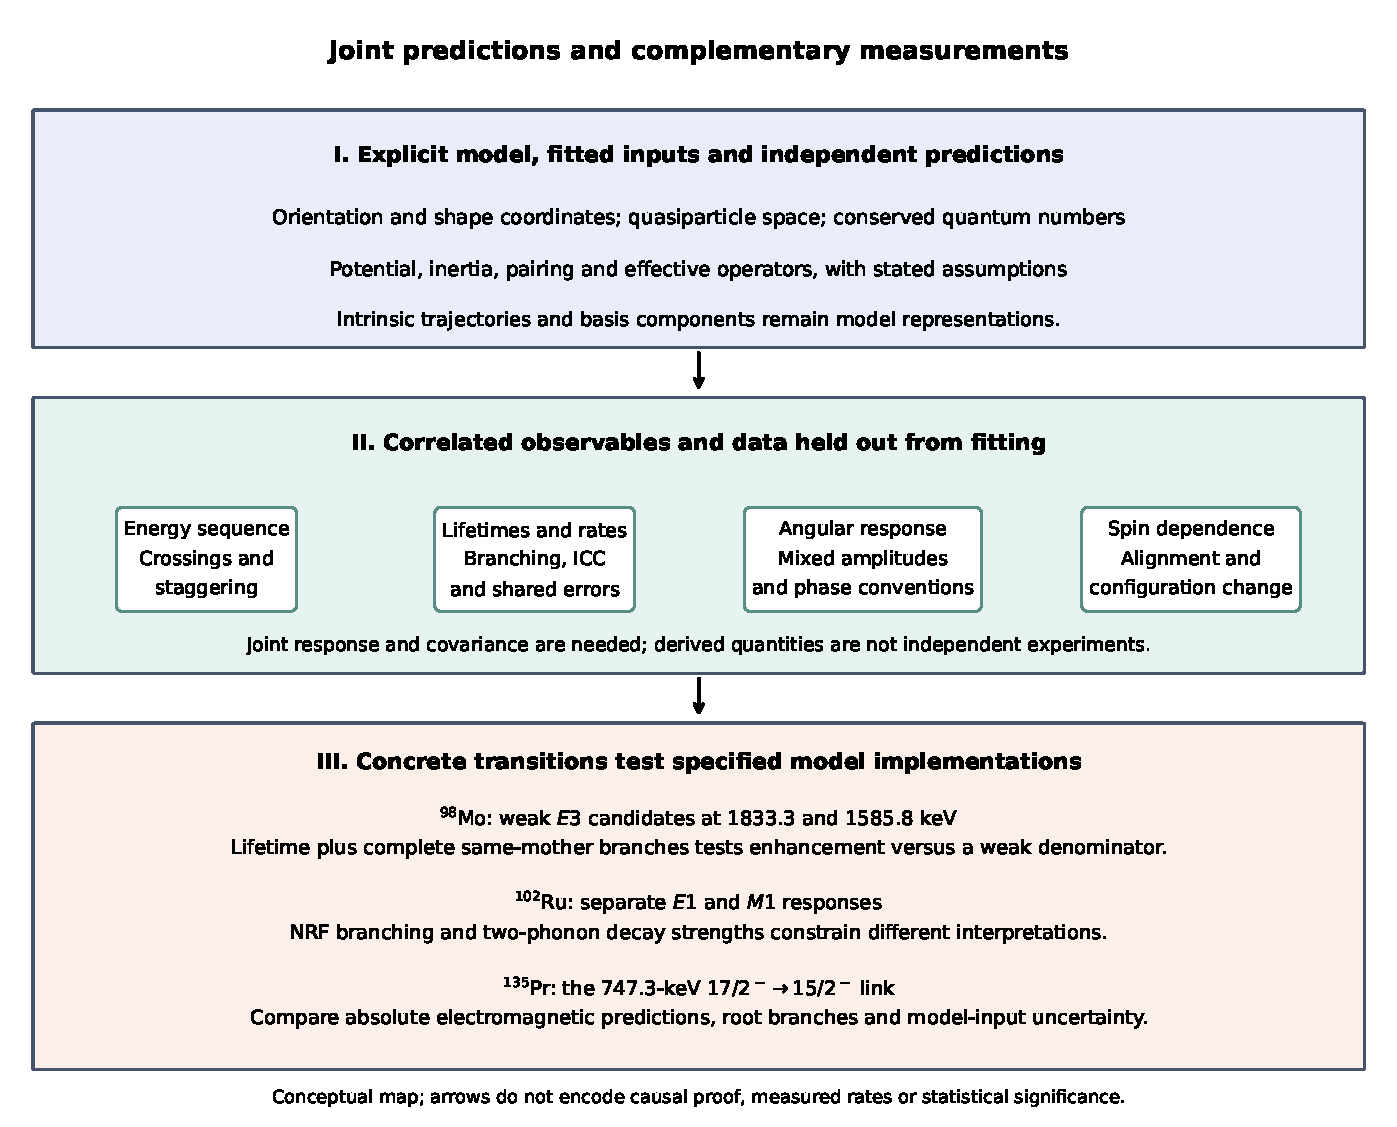
\includegraphics[width=0.88\textwidth]{Img/joint-predictions-workflow.pdf}
\caption[模式判断需要怎样的联合预言：理论前向预言架构、互补信息通道与实证研究候选逻辑框架示意图]{模式判断需要怎样的联合预言：理论前向预言架构、互补信息通道与实证研究候选逻辑框架示意图。图示展示了从理论模型自由度划分与输入设定出发，经由多通道关联实验观测（能级序列、绝对衰变速率、方向角关联双根与偏振度、高自旋顺排响应），最终落地于具体可证伪实证候选的科学闭环；代码实现与数据来源参见附录\ref{app:reproducible-inputs}。}\label{fig:3-8-joint-workflow}
\end{figure}

当将某一特定核区（如 $A \approx 130$ 区）总结出的模式机制推广迁移至其它质量区时，必须严格遵守微观自洽的物理迁移准则：
\begin{itemize}
\item 必须逐一核查目标核区的微观费米面轨道占据情况、自旋-轨道伴对轨道的相对劈裂、质子-中子残余相互作用的有效强度（如Ding 等人在 $A \approx 60$ 钴同位素探索性三轴粒子-转子计算中对残余力 $V_{pn}$ 与取向进动边界的系统考察~\cite{ding-2025-chiral-rotation-a60-residual-interactions}）、自洽平均场势能面的三轴刚度、以及在束反应布居通道的角动量输入特征。
\item 不能仅因某个质量数区间与已知变形核相近，或因文献暂缺，便断言新模式的『确证』或『缺失』。原子核的多体激发动力学由其微观壳层结构与哈密顿量本征态决定，模式判断应以具体实验证据与反例检验为准。
\end{itemize}

综上所述，将一个理论模式确立为真实客观的核物理激发，绝非依赖孤立的能谱拟合或人为的模式命名，而是依赖于一组具有互补信息维度、相互自洽的联合预言链条。通过建立包含绝对寿命、多角度偏振分析、高自旋顺排演化以及严格考量统计协方差的多维观测体系，并面向具体实证候选开展判决性测量，才能真正打破模型解释简并，将低能核结构高自旋谱学研究推进至自洽严谨的科学高度。
%
}{%
    \section{模式判断需要怎样的联合预言 [未完成]}\label{sec:3-8}%
    \textit{本节尚未完成。}%
}
